% Created by tikzDevice version 0.10.1 on 2016-06-15 07:23:57
% !TEX encoding = UTF-8 Unicode
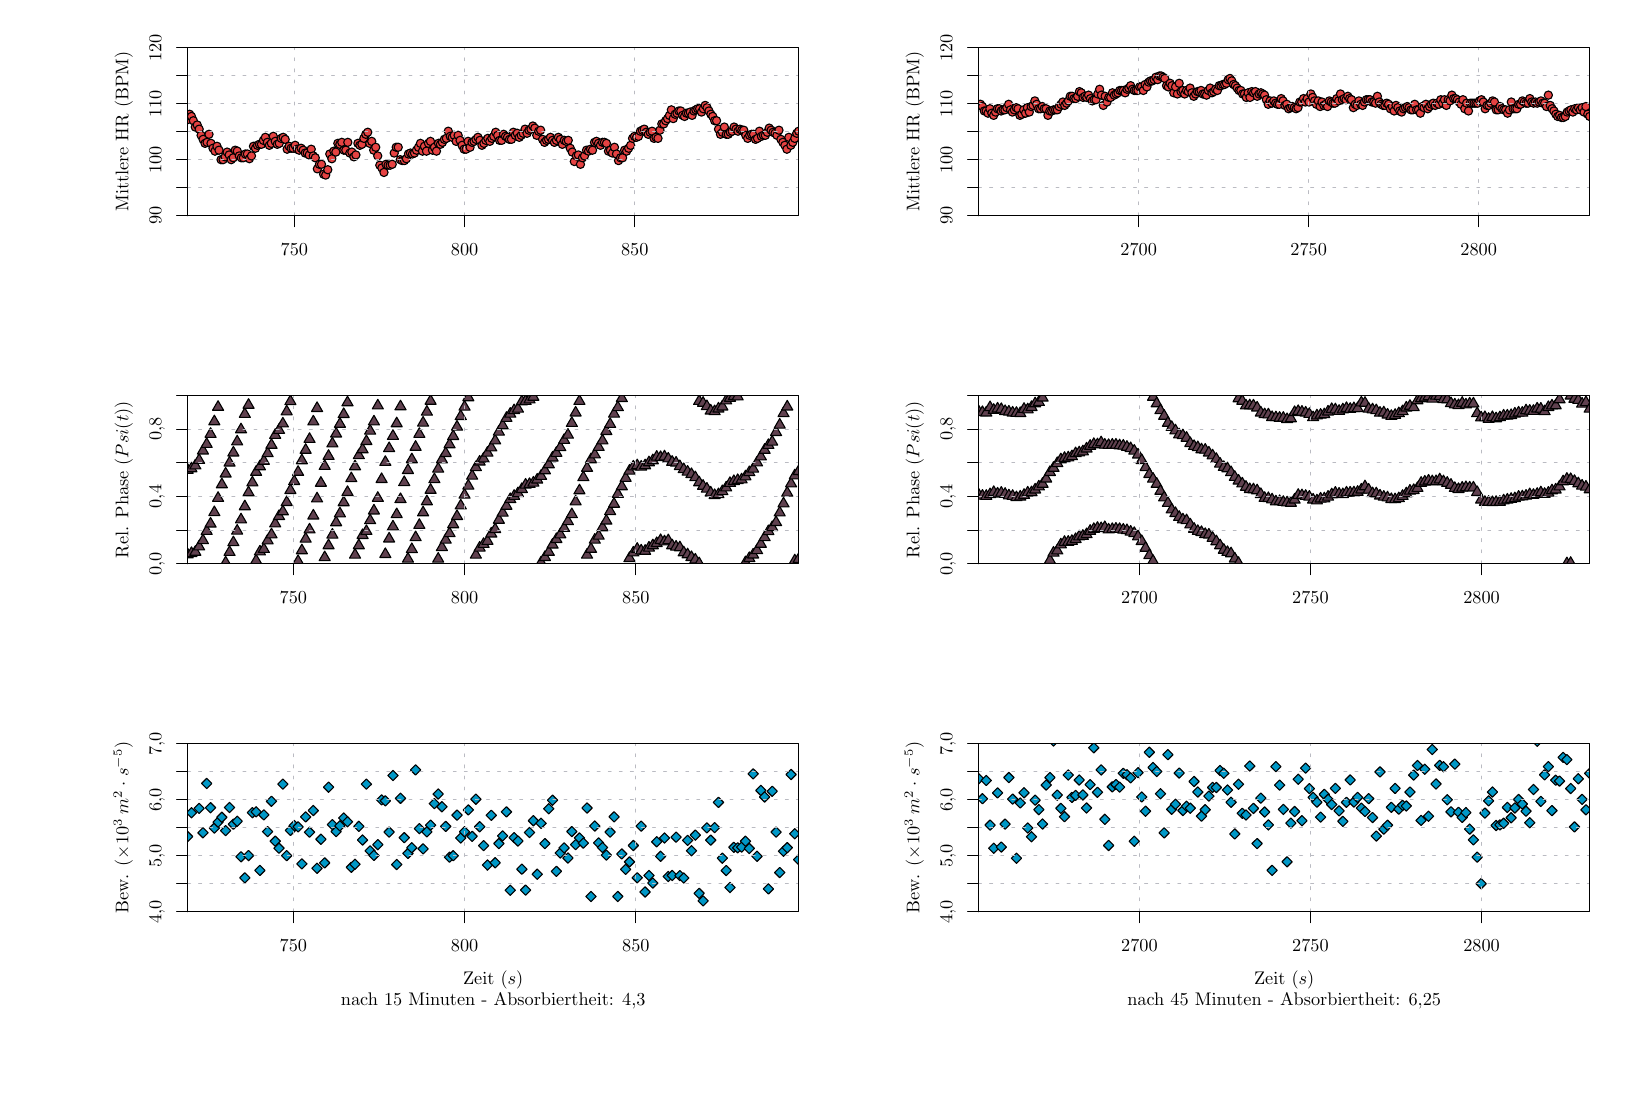
\begin{tikzpicture}[x=1pt,y=1pt]
\definecolor{fillColor}{RGB}{255,255,255}
\path[use as bounding box,fill=fillColor,fill opacity=0.00] (0,0) rectangle (571.66,377.25);
\begin{scope}
\path[clip] ( 57.82,309.32) rectangle (278.60,370.02);
\definecolor{drawColor}{RGB}{0,0,0}
\definecolor{fillColor}{RGB}{229,66,66}

\path[draw=drawColor,line width= 0.4pt,line join=round,line cap=round,fill=fillColor] ( 57.82,344.01) circle (  1.49);

\path[draw=drawColor,line width= 0.4pt,line join=round,line cap=round,fill=fillColor] ( 58.50,345.96) circle (  1.49);

\path[draw=drawColor,line width= 0.4pt,line join=round,line cap=round,fill=fillColor] ( 59.18,345.17) circle (  1.49);

\path[draw=drawColor,line width= 0.4pt,line join=round,line cap=round,fill=fillColor] ( 59.87,343.62) circle (  1.49);

\path[draw=drawColor,line width= 0.4pt,line join=round,line cap=round,fill=fillColor] ( 60.57,341.33) circle (  1.49);

\path[draw=drawColor,line width= 0.4pt,line join=round,line cap=round,fill=fillColor] ( 61.27,342.09) circle (  1.49);

\path[draw=drawColor,line width= 0.4pt,line join=round,line cap=round,fill=fillColor] ( 61.97,340.58) circle (  1.49);

\path[draw=drawColor,line width= 0.4pt,line join=round,line cap=round,fill=fillColor] ( 62.67,338.35) circle (  1.49);

\path[draw=drawColor,line width= 0.4pt,line join=round,line cap=round,fill=fillColor] ( 63.39,336.89) circle (  1.49);

\path[draw=drawColor,line width= 0.4pt,line join=round,line cap=round,fill=fillColor] ( 64.10,335.45) circle (  1.49);

\path[draw=drawColor,line width= 0.4pt,line join=round,line cap=round,fill=fillColor] ( 64.82,335.81) circle (  1.49);

\path[draw=drawColor,line width= 0.4pt,line join=round,line cap=round,fill=fillColor] ( 65.52,338.72) circle (  1.49);

\path[draw=drawColor,line width= 0.4pt,line join=round,line cap=round,fill=fillColor] ( 66.24,335.45) circle (  1.49);

\path[draw=drawColor,line width= 0.4pt,line join=round,line cap=round,fill=fillColor] ( 66.96,333.68) circle (  1.49);

\path[draw=drawColor,line width= 0.4pt,line join=round,line cap=round,fill=fillColor] ( 67.69,332.63) circle (  1.49);

\path[draw=drawColor,line width= 0.4pt,line join=round,line cap=round,fill=fillColor] ( 68.41,334.39) circle (  1.49);

\path[draw=drawColor,line width= 0.4pt,line join=round,line cap=round,fill=fillColor] ( 69.14,332.98) circle (  1.49);

\path[draw=drawColor,line width= 0.4pt,line join=round,line cap=round,fill=fillColor] ( 69.88,329.55) circle (  1.49);

\path[draw=drawColor,line width= 0.4pt,line join=round,line cap=round,fill=fillColor] ( 70.61,329.55) circle (  1.49);

\path[draw=drawColor,line width= 0.4pt,line join=round,line cap=round,fill=fillColor] ( 71.35,330.57) circle (  1.49);

\path[draw=drawColor,line width= 0.4pt,line join=round,line cap=round,fill=fillColor] ( 72.08,332.29) circle (  1.49);

\path[draw=drawColor,line width= 0.4pt,line join=round,line cap=round,fill=fillColor] ( 72.81,331.25) circle (  1.49);

\path[draw=drawColor,line width= 0.4pt,line join=round,line cap=round,fill=fillColor] ( 73.55,329.55) circle (  1.49);

\path[draw=drawColor,line width= 0.4pt,line join=round,line cap=round,fill=fillColor] ( 74.28,330.23) circle (  1.49);

\path[draw=drawColor,line width= 0.4pt,line join=round,line cap=round,fill=fillColor] ( 75.01,332.98) circle (  1.49);

\path[draw=drawColor,line width= 0.4pt,line join=round,line cap=round,fill=fillColor] ( 75.74,332.63) circle (  1.49);

\path[draw=drawColor,line width= 0.4pt,line join=round,line cap=round,fill=fillColor] ( 76.47,330.91) circle (  1.49);

\path[draw=drawColor,line width= 0.4pt,line join=round,line cap=round,fill=fillColor] ( 77.20,330.23) circle (  1.49);

\path[draw=drawColor,line width= 0.4pt,line join=round,line cap=round,fill=fillColor] ( 77.94,330.23) circle (  1.49);

\path[draw=drawColor,line width= 0.4pt,line join=round,line cap=round,fill=fillColor] ( 78.67,331.60) circle (  1.49);

\path[draw=drawColor,line width= 0.4pt,line join=round,line cap=round,fill=fillColor] ( 79.40,331.60) circle (  1.49);

\path[draw=drawColor,line width= 0.4pt,line join=round,line cap=round,fill=fillColor] ( 80.14,329.89) circle (  1.49);

\path[draw=drawColor,line width= 0.4pt,line join=round,line cap=round,fill=fillColor] ( 80.87,330.91) circle (  1.49);

\path[draw=drawColor,line width= 0.4pt,line join=round,line cap=round,fill=fillColor] ( 81.59,334.39) circle (  1.49);

\path[draw=drawColor,line width= 0.4pt,line join=round,line cap=round,fill=fillColor] ( 82.31,333.68) circle (  1.49);

\path[draw=drawColor,line width= 0.4pt,line join=round,line cap=round,fill=fillColor] ( 83.03,334.74) circle (  1.49);

\path[draw=drawColor,line width= 0.4pt,line join=round,line cap=round,fill=fillColor] ( 83.75,335.10) circle (  1.49);

\path[draw=drawColor,line width= 0.4pt,line join=round,line cap=round,fill=fillColor] ( 84.47,335.10) circle (  1.49);

\path[draw=drawColor,line width= 0.4pt,line join=round,line cap=round,fill=fillColor] ( 85.18,336.53) circle (  1.49);

\path[draw=drawColor,line width= 0.4pt,line join=round,line cap=round,fill=fillColor] ( 85.89,337.62) circle (  1.49);

\path[draw=drawColor,line width= 0.4pt,line join=round,line cap=round,fill=fillColor] ( 86.61,335.81) circle (  1.49);

\path[draw=drawColor,line width= 0.4pt,line join=round,line cap=round,fill=fillColor] ( 87.33,334.74) circle (  1.49);

\path[draw=drawColor,line width= 0.4pt,line join=round,line cap=round,fill=fillColor] ( 88.05,335.45) circle (  1.49);

\path[draw=drawColor,line width= 0.4pt,line join=round,line cap=round,fill=fillColor] ( 88.75,337.98) circle (  1.49);

\path[draw=drawColor,line width= 0.4pt,line join=round,line cap=round,fill=fillColor] ( 89.47,336.17) circle (  1.49);

\path[draw=drawColor,line width= 0.4pt,line join=round,line cap=round,fill=fillColor] ( 90.19,335.10) circle (  1.49);

\path[draw=drawColor,line width= 0.4pt,line join=round,line cap=round,fill=fillColor] ( 90.90,335.45) circle (  1.49);

\path[draw=drawColor,line width= 0.4pt,line join=round,line cap=round,fill=fillColor] ( 91.62,337.25) circle (  1.49);

\path[draw=drawColor,line width= 0.4pt,line join=round,line cap=round,fill=fillColor] ( 92.33,337.62) circle (  1.49);

\path[draw=drawColor,line width= 0.4pt,line join=round,line cap=round,fill=fillColor] ( 93.04,336.89) circle (  1.49);

\path[draw=drawColor,line width= 0.4pt,line join=round,line cap=round,fill=fillColor] ( 93.76,333.33) circle (  1.49);

\path[draw=drawColor,line width= 0.4pt,line join=round,line cap=round,fill=fillColor] ( 94.48,334.39) circle (  1.49);

\path[draw=drawColor,line width= 0.4pt,line join=round,line cap=round,fill=fillColor] ( 95.21,333.68) circle (  1.49);

\path[draw=drawColor,line width= 0.4pt,line join=round,line cap=round,fill=fillColor] ( 95.93,333.68) circle (  1.49);

\path[draw=drawColor,line width= 0.4pt,line join=round,line cap=round,fill=fillColor] ( 96.65,334.74) circle (  1.49);

\path[draw=drawColor,line width= 0.4pt,line join=round,line cap=round,fill=fillColor] ( 97.37,333.33) circle (  1.49);

\path[draw=drawColor,line width= 0.4pt,line join=round,line cap=round,fill=fillColor] ( 98.10,332.98) circle (  1.49);

\path[draw=drawColor,line width= 0.4pt,line join=round,line cap=round,fill=fillColor] ( 98.82,333.68) circle (  1.49);

\path[draw=drawColor,line width= 0.4pt,line join=round,line cap=round,fill=fillColor] ( 99.55,332.98) circle (  1.49);

\path[draw=drawColor,line width= 0.4pt,line join=round,line cap=round,fill=fillColor] (100.28,331.94) circle (  1.49);

\path[draw=drawColor,line width= 0.4pt,line join=round,line cap=round,fill=fillColor] (101.01,331.94) circle (  1.49);

\path[draw=drawColor,line width= 0.4pt,line join=round,line cap=round,fill=fillColor] (101.74,331.25) circle (  1.49);

\path[draw=drawColor,line width= 0.4pt,line join=round,line cap=round,fill=fillColor] (102.46,333.33) circle (  1.49);

\path[draw=drawColor,line width= 0.4pt,line join=round,line cap=round,fill=fillColor] (103.20,330.91) circle (  1.49);

\path[draw=drawColor,line width= 0.4pt,line join=round,line cap=round,fill=fillColor] (103.93,330.23) circle (  1.49);

\path[draw=drawColor,line width= 0.4pt,line join=round,line cap=round,fill=fillColor] (104.68,326.23) circle (  1.49);

\path[draw=drawColor,line width= 0.4pt,line join=round,line cap=round,fill=fillColor] (105.43,327.88) circle (  1.49);

\path[draw=drawColor,line width= 0.4pt,line join=round,line cap=round,fill=fillColor] (106.17,327.88) circle (  1.49);

\path[draw=drawColor,line width= 0.4pt,line join=round,line cap=round,fill=fillColor] (106.93,324.30) circle (  1.49);

\path[draw=drawColor,line width= 0.4pt,line join=round,line cap=round,fill=fillColor] (107.69,323.98) circle (  1.49);

\path[draw=drawColor,line width= 0.4pt,line join=round,line cap=round,fill=fillColor] (108.44,325.91) circle (  1.49);

\path[draw=drawColor,line width= 0.4pt,line join=round,line cap=round,fill=fillColor] (109.17,331.60) circle (  1.49);

\path[draw=drawColor,line width= 0.4pt,line join=round,line cap=round,fill=fillColor] (109.91,329.89) circle (  1.49);

\path[draw=drawColor,line width= 0.4pt,line join=round,line cap=round,fill=fillColor] (110.63,332.63) circle (  1.49);

\path[draw=drawColor,line width= 0.4pt,line join=round,line cap=round,fill=fillColor] (111.36,332.29) circle (  1.49);

\path[draw=drawColor,line width= 0.4pt,line join=round,line cap=round,fill=fillColor] (112.08,335.45) circle (  1.49);

\path[draw=drawColor,line width= 0.4pt,line join=round,line cap=round,fill=fillColor] (112.80,335.10) circle (  1.49);

\path[draw=drawColor,line width= 0.4pt,line join=round,line cap=round,fill=fillColor] (113.51,335.81) circle (  1.49);

\path[draw=drawColor,line width= 0.4pt,line join=round,line cap=round,fill=fillColor] (114.24,332.98) circle (  1.49);

\path[draw=drawColor,line width= 0.4pt,line join=round,line cap=round,fill=fillColor] (114.96,332.98) circle (  1.49);

\path[draw=drawColor,line width= 0.4pt,line join=round,line cap=round,fill=fillColor] (115.68,335.81) circle (  1.49);

\path[draw=drawColor,line width= 0.4pt,line join=round,line cap=round,fill=fillColor] (116.41,331.94) circle (  1.49);

\path[draw=drawColor,line width= 0.4pt,line join=round,line cap=round,fill=fillColor] (117.14,332.29) circle (  1.49);

\path[draw=drawColor,line width= 0.4pt,line join=round,line cap=round,fill=fillColor] (117.87,330.57) circle (  1.49);

\path[draw=drawColor,line width= 0.4pt,line join=round,line cap=round,fill=fillColor] (118.60,331.25) circle (  1.49);

\path[draw=drawColor,line width= 0.4pt,line join=round,line cap=round,fill=fillColor] (119.32,335.45) circle (  1.49);

\path[draw=drawColor,line width= 0.4pt,line join=round,line cap=round,fill=fillColor] (120.04,334.74) circle (  1.49);

\path[draw=drawColor,line width= 0.4pt,line join=round,line cap=round,fill=fillColor] (120.76,335.10) circle (  1.49);

\path[draw=drawColor,line width= 0.4pt,line join=round,line cap=round,fill=fillColor] (121.47,337.25) circle (  1.49);

\path[draw=drawColor,line width= 0.4pt,line join=round,line cap=round,fill=fillColor] (122.18,338.72) circle (  1.49);

\path[draw=drawColor,line width= 0.4pt,line join=round,line cap=round,fill=fillColor] (122.88,339.46) circle (  1.49);

\path[draw=drawColor,line width= 0.4pt,line join=round,line cap=round,fill=fillColor] (123.60,335.45) circle (  1.49);

\path[draw=drawColor,line width= 0.4pt,line join=round,line cap=round,fill=fillColor] (124.31,336.17) circle (  1.49);

\path[draw=drawColor,line width= 0.4pt,line join=round,line cap=round,fill=fillColor] (125.04,332.98) circle (  1.49);

\path[draw=drawColor,line width= 0.4pt,line join=round,line cap=round,fill=fillColor] (125.76,334.03) circle (  1.49);

\path[draw=drawColor,line width= 0.4pt,line join=round,line cap=round,fill=fillColor] (126.49,330.91) circle (  1.49);

\path[draw=drawColor,line width= 0.4pt,line join=round,line cap=round,fill=fillColor] (127.24,327.55) circle (  1.49);

\path[draw=drawColor,line width= 0.4pt,line join=round,line cap=round,fill=fillColor] (127.99,326.56) circle (  1.49);

\path[draw=drawColor,line width= 0.4pt,line join=round,line cap=round,fill=fillColor] (128.74,324.94) circle (  1.49);

\path[draw=drawColor,line width= 0.4pt,line join=round,line cap=round,fill=fillColor] (129.49,327.88) circle (  1.49);

\path[draw=drawColor,line width= 0.4pt,line join=round,line cap=round,fill=fillColor] (130.23,327.55) circle (  1.49);

\path[draw=drawColor,line width= 0.4pt,line join=round,line cap=round,fill=fillColor] (130.98,327.55) circle (  1.49);

\path[draw=drawColor,line width= 0.4pt,line join=round,line cap=round,fill=fillColor] (131.72,327.88) circle (  1.49);

\path[draw=drawColor,line width= 0.4pt,line join=round,line cap=round,fill=fillColor] (132.45,331.94) circle (  1.49);

\path[draw=drawColor,line width= 0.4pt,line join=round,line cap=round,fill=fillColor] (133.17,334.03) circle (  1.49);

\path[draw=drawColor,line width= 0.4pt,line join=round,line cap=round,fill=fillColor] (133.89,334.03) circle (  1.49);

\path[draw=drawColor,line width= 0.4pt,line join=round,line cap=round,fill=fillColor] (134.63,329.55) circle (  1.49);

\path[draw=drawColor,line width= 0.4pt,line join=round,line cap=round,fill=fillColor] (135.37,329.21) circle (  1.49);

\path[draw=drawColor,line width= 0.4pt,line join=round,line cap=round,fill=fillColor] (136.11,329.21) circle (  1.49);

\path[draw=drawColor,line width= 0.4pt,line join=round,line cap=round,fill=fillColor] (136.85,329.89) circle (  1.49);

\path[draw=drawColor,line width= 0.4pt,line join=round,line cap=round,fill=fillColor] (137.58,331.60) circle (  1.49);

\path[draw=drawColor,line width= 0.4pt,line join=round,line cap=round,fill=fillColor] (138.31,331.94) circle (  1.49);

\path[draw=drawColor,line width= 0.4pt,line join=round,line cap=round,fill=fillColor] (139.04,331.60) circle (  1.49);

\path[draw=drawColor,line width= 0.4pt,line join=round,line cap=round,fill=fillColor] (139.77,331.94) circle (  1.49);

\path[draw=drawColor,line width= 0.4pt,line join=round,line cap=round,fill=fillColor] (140.49,332.98) circle (  1.49);

\path[draw=drawColor,line width= 0.4pt,line join=round,line cap=round,fill=fillColor] (141.22,334.03) circle (  1.49);

\path[draw=drawColor,line width= 0.4pt,line join=round,line cap=round,fill=fillColor] (141.93,335.45) circle (  1.49);

\path[draw=drawColor,line width= 0.4pt,line join=round,line cap=round,fill=fillColor] (142.66,332.63) circle (  1.49);

\path[draw=drawColor,line width= 0.4pt,line join=round,line cap=round,fill=fillColor] (143.38,334.39) circle (  1.49);

\path[draw=drawColor,line width= 0.4pt,line join=round,line cap=round,fill=fillColor] (144.11,332.63) circle (  1.49);

\path[draw=drawColor,line width= 0.4pt,line join=round,line cap=round,fill=fillColor] (144.82,335.45) circle (  1.49);

\path[draw=drawColor,line width= 0.4pt,line join=round,line cap=round,fill=fillColor] (145.54,336.17) circle (  1.49);

\path[draw=drawColor,line width= 0.4pt,line join=round,line cap=round,fill=fillColor] (146.26,332.98) circle (  1.49);

\path[draw=drawColor,line width= 0.4pt,line join=round,line cap=round,fill=fillColor] (146.99,334.03) circle (  1.49);

\path[draw=drawColor,line width= 0.4pt,line join=round,line cap=round,fill=fillColor] (147.71,332.63) circle (  1.49);

\path[draw=drawColor,line width= 0.4pt,line join=round,line cap=round,fill=fillColor] (148.43,335.45) circle (  1.49);

\path[draw=drawColor,line width= 0.4pt,line join=round,line cap=round,fill=fillColor] (149.15,335.10) circle (  1.49);

\path[draw=drawColor,line width= 0.4pt,line join=round,line cap=round,fill=fillColor] (149.87,335.81) circle (  1.49);

\path[draw=drawColor,line width= 0.4pt,line join=round,line cap=round,fill=fillColor] (150.58,336.89) circle (  1.49);

\path[draw=drawColor,line width= 0.4pt,line join=round,line cap=round,fill=fillColor] (151.29,337.25) circle (  1.49);

\path[draw=drawColor,line width= 0.4pt,line join=round,line cap=round,fill=fillColor] (151.99,339.83) circle (  1.49);

\path[draw=drawColor,line width= 0.4pt,line join=round,line cap=round,fill=fillColor] (152.70,337.98) circle (  1.49);

\path[draw=drawColor,line width= 0.4pt,line join=round,line cap=round,fill=fillColor] (153.41,337.62) circle (  1.49);

\path[draw=drawColor,line width= 0.4pt,line join=round,line cap=round,fill=fillColor] (154.12,338.35) circle (  1.49);

\path[draw=drawColor,line width= 0.4pt,line join=round,line cap=round,fill=fillColor] (154.83,336.17) circle (  1.49);

\path[draw=drawColor,line width= 0.4pt,line join=round,line cap=round,fill=fillColor] (155.54,338.35) circle (  1.49);

\path[draw=drawColor,line width= 0.4pt,line join=round,line cap=round,fill=fillColor] (156.25,336.53) circle (  1.49);

\path[draw=drawColor,line width= 0.4pt,line join=round,line cap=round,fill=fillColor] (156.97,334.74) circle (  1.49);

\path[draw=drawColor,line width= 0.4pt,line join=round,line cap=round,fill=fillColor] (157.70,333.33) circle (  1.49);

\path[draw=drawColor,line width= 0.4pt,line join=round,line cap=round,fill=fillColor] (158.42,333.33) circle (  1.49);

\path[draw=drawColor,line width= 0.4pt,line join=round,line cap=round,fill=fillColor] (159.13,336.17) circle (  1.49);

\path[draw=drawColor,line width= 0.4pt,line join=round,line cap=round,fill=fillColor] (159.86,334.03) circle (  1.49);

\path[draw=drawColor,line width= 0.4pt,line join=round,line cap=round,fill=fillColor] (160.57,335.81) circle (  1.49);

\path[draw=drawColor,line width= 0.4pt,line join=round,line cap=round,fill=fillColor] (161.29,336.17) circle (  1.49);

\path[draw=drawColor,line width= 0.4pt,line join=round,line cap=round,fill=fillColor] (162.00,336.89) circle (  1.49);

\path[draw=drawColor,line width= 0.4pt,line join=round,line cap=round,fill=fillColor] (162.71,337.62) circle (  1.49);

\path[draw=drawColor,line width= 0.4pt,line join=round,line cap=round,fill=fillColor] (163.42,336.53) circle (  1.49);

\path[draw=drawColor,line width= 0.4pt,line join=round,line cap=round,fill=fillColor] (164.14,334.74) circle (  1.49);

\path[draw=drawColor,line width= 0.4pt,line join=round,line cap=round,fill=fillColor] (164.86,335.45) circle (  1.49);

\path[draw=drawColor,line width= 0.4pt,line join=round,line cap=round,fill=fillColor] (165.57,336.53) circle (  1.49);

\path[draw=drawColor,line width= 0.4pt,line join=round,line cap=round,fill=fillColor] (166.28,337.25) circle (  1.49);

\path[draw=drawColor,line width= 0.4pt,line join=round,line cap=round,fill=fillColor] (167.00,336.17) circle (  1.49);

\path[draw=drawColor,line width= 0.4pt,line join=round,line cap=round,fill=fillColor] (167.71,337.25) circle (  1.49);

\path[draw=drawColor,line width= 0.4pt,line join=round,line cap=round,fill=fillColor] (168.42,337.98) circle (  1.49);

\path[draw=drawColor,line width= 0.4pt,line join=round,line cap=round,fill=fillColor] (169.12,339.46) circle (  1.49);

\path[draw=drawColor,line width= 0.4pt,line join=round,line cap=round,fill=fillColor] (169.83,338.35) circle (  1.49);

\path[draw=drawColor,line width= 0.4pt,line join=round,line cap=round,fill=fillColor] (170.54,336.53) circle (  1.49);

\path[draw=drawColor,line width= 0.4pt,line join=round,line cap=round,fill=fillColor] (171.26,336.53) circle (  1.49);

\path[draw=drawColor,line width= 0.4pt,line join=round,line cap=round,fill=fillColor] (171.96,338.72) circle (  1.49);

\path[draw=drawColor,line width= 0.4pt,line join=round,line cap=round,fill=fillColor] (172.67,337.98) circle (  1.49);

\path[draw=drawColor,line width= 0.4pt,line join=round,line cap=round,fill=fillColor] (173.38,337.62) circle (  1.49);

\path[draw=drawColor,line width= 0.4pt,line join=round,line cap=round,fill=fillColor] (174.09,336.89) circle (  1.49);

\path[draw=drawColor,line width= 0.4pt,line join=round,line cap=round,fill=fillColor] (174.80,336.89) circle (  1.49);

\path[draw=drawColor,line width= 0.4pt,line join=round,line cap=round,fill=fillColor] (175.51,339.46) circle (  1.49);

\path[draw=drawColor,line width= 0.4pt,line join=round,line cap=round,fill=fillColor] (176.21,338.35) circle (  1.49);

\path[draw=drawColor,line width= 0.4pt,line join=round,line cap=round,fill=fillColor] (176.92,339.09) circle (  1.49);

\path[draw=drawColor,line width= 0.4pt,line join=round,line cap=round,fill=fillColor] (177.63,337.62) circle (  1.49);

\path[draw=drawColor,line width= 0.4pt,line join=round,line cap=round,fill=fillColor] (178.34,338.35) circle (  1.49);

\path[draw=drawColor,line width= 0.4pt,line join=round,line cap=round,fill=fillColor] (179.04,339.09) circle (  1.49);

\path[draw=drawColor,line width= 0.4pt,line join=round,line cap=round,fill=fillColor] (179.74,340.58) circle (  1.49);

\path[draw=drawColor,line width= 0.4pt,line join=round,line cap=round,fill=fillColor] (180.45,339.09) circle (  1.49);

\path[draw=drawColor,line width= 0.4pt,line join=round,line cap=round,fill=fillColor] (181.15,340.20) circle (  1.49);

\path[draw=drawColor,line width= 0.4pt,line join=round,line cap=round,fill=fillColor] (181.85,340.58) circle (  1.49);

\path[draw=drawColor,line width= 0.4pt,line join=round,line cap=round,fill=fillColor] (182.54,341.71) circle (  1.49);

\path[draw=drawColor,line width= 0.4pt,line join=round,line cap=round,fill=fillColor] (183.24,340.95) circle (  1.49);

\path[draw=drawColor,line width= 0.4pt,line join=round,line cap=round,fill=fillColor] (183.95,338.35) circle (  1.49);

\path[draw=drawColor,line width= 0.4pt,line join=round,line cap=round,fill=fillColor] (184.65,339.83) circle (  1.49);

\path[draw=drawColor,line width= 0.4pt,line join=round,line cap=round,fill=fillColor] (185.35,340.20) circle (  1.49);

\path[draw=drawColor,line width= 0.4pt,line join=round,line cap=round,fill=fillColor] (186.06,336.89) circle (  1.49);

\path[draw=drawColor,line width= 0.4pt,line join=round,line cap=round,fill=fillColor] (186.78,335.81) circle (  1.49);

\path[draw=drawColor,line width= 0.4pt,line join=round,line cap=round,fill=fillColor] (187.49,336.53) circle (  1.49);

\path[draw=drawColor,line width= 0.4pt,line join=round,line cap=round,fill=fillColor] (188.21,336.89) circle (  1.49);

\path[draw=drawColor,line width= 0.4pt,line join=round,line cap=round,fill=fillColor] (188.92,337.62) circle (  1.49);

\path[draw=drawColor,line width= 0.4pt,line join=round,line cap=round,fill=fillColor] (189.63,336.53) circle (  1.49);

\path[draw=drawColor,line width= 0.4pt,line join=round,line cap=round,fill=fillColor] (190.35,335.81) circle (  1.49);

\path[draw=drawColor,line width= 0.4pt,line join=round,line cap=round,fill=fillColor] (191.06,336.53) circle (  1.49);

\path[draw=drawColor,line width= 0.4pt,line join=round,line cap=round,fill=fillColor] (191.77,337.62) circle (  1.49);

\path[draw=drawColor,line width= 0.4pt,line join=round,line cap=round,fill=fillColor] (192.48,336.89) circle (  1.49);

\path[draw=drawColor,line width= 0.4pt,line join=round,line cap=round,fill=fillColor] (193.20,335.10) circle (  1.49);

\path[draw=drawColor,line width= 0.4pt,line join=round,line cap=round,fill=fillColor] (193.91,336.53) circle (  1.49);

\path[draw=drawColor,line width= 0.4pt,line join=round,line cap=round,fill=fillColor] (194.63,336.17) circle (  1.49);

\path[draw=drawColor,line width= 0.4pt,line join=round,line cap=round,fill=fillColor] (195.34,336.53) circle (  1.49);

\path[draw=drawColor,line width= 0.4pt,line join=round,line cap=round,fill=fillColor] (196.06,333.68) circle (  1.49);

\path[draw=drawColor,line width= 0.4pt,line join=round,line cap=round,fill=fillColor] (196.79,332.29) circle (  1.49);

\path[draw=drawColor,line width= 0.4pt,line join=round,line cap=round,fill=fillColor] (197.53,328.88) circle (  1.49);

\path[draw=drawColor,line width= 0.4pt,line join=round,line cap=round,fill=fillColor] (198.27,330.91) circle (  1.49);

\path[draw=drawColor,line width= 0.4pt,line join=round,line cap=round,fill=fillColor] (199.00,331.25) circle (  1.49);

\path[draw=drawColor,line width= 0.4pt,line join=round,line cap=round,fill=fillColor] (199.74,327.88) circle (  1.49);

\path[draw=drawColor,line width= 0.4pt,line join=round,line cap=round,fill=fillColor] (200.48,330.23) circle (  1.49);

\path[draw=drawColor,line width= 0.4pt,line join=round,line cap=round,fill=fillColor] (201.21,330.91) circle (  1.49);

\path[draw=drawColor,line width= 0.4pt,line join=round,line cap=round,fill=fillColor] (201.94,332.98) circle (  1.49);

\path[draw=drawColor,line width= 0.4pt,line join=round,line cap=round,fill=fillColor] (202.66,332.63) circle (  1.49);

\path[draw=drawColor,line width= 0.4pt,line join=round,line cap=round,fill=fillColor] (203.39,333.33) circle (  1.49);

\path[draw=drawColor,line width= 0.4pt,line join=round,line cap=round,fill=fillColor] (204.11,332.98) circle (  1.49);

\path[draw=drawColor,line width= 0.4pt,line join=round,line cap=round,fill=fillColor] (204.83,335.81) circle (  1.49);

\path[draw=drawColor,line width= 0.4pt,line join=round,line cap=round,fill=fillColor] (205.54,336.17) circle (  1.49);

\path[draw=drawColor,line width= 0.4pt,line join=round,line cap=round,fill=fillColor] (206.26,335.45) circle (  1.49);

\path[draw=drawColor,line width= 0.4pt,line join=round,line cap=round,fill=fillColor] (206.98,334.74) circle (  1.49);

\path[draw=drawColor,line width= 0.4pt,line join=round,line cap=round,fill=fillColor] (207.70,335.81) circle (  1.49);

\path[draw=drawColor,line width= 0.4pt,line join=round,line cap=round,fill=fillColor] (208.41,335.81) circle (  1.49);

\path[draw=drawColor,line width= 0.4pt,line join=round,line cap=round,fill=fillColor] (209.13,335.45) circle (  1.49);

\path[draw=drawColor,line width= 0.4pt,line join=round,line cap=round,fill=fillColor] (209.86,332.63) circle (  1.49);

\path[draw=drawColor,line width= 0.4pt,line join=round,line cap=round,fill=fillColor] (210.58,332.98) circle (  1.49);

\path[draw=drawColor,line width= 0.4pt,line join=round,line cap=round,fill=fillColor] (211.31,331.94) circle (  1.49);

\path[draw=drawColor,line width= 0.4pt,line join=round,line cap=round,fill=fillColor] (212.03,334.03) circle (  1.49);

\path[draw=drawColor,line width= 0.4pt,line join=round,line cap=round,fill=fillColor] (212.76,331.60) circle (  1.49);

\path[draw=drawColor,line width= 0.4pt,line join=round,line cap=round,fill=fillColor] (213.50,329.21) circle (  1.49);

\path[draw=drawColor,line width= 0.4pt,line join=round,line cap=round,fill=fillColor] (214.24,330.23) circle (  1.49);

\path[draw=drawColor,line width= 0.4pt,line join=round,line cap=round,fill=fillColor] (214.97,330.23) circle (  1.49);

\path[draw=drawColor,line width= 0.4pt,line join=round,line cap=round,fill=fillColor] (215.70,332.98) circle (  1.49);

\path[draw=drawColor,line width= 0.4pt,line join=round,line cap=round,fill=fillColor] (216.43,332.63) circle (  1.49);

\path[draw=drawColor,line width= 0.4pt,line join=round,line cap=round,fill=fillColor] (217.15,333.68) circle (  1.49);

\path[draw=drawColor,line width= 0.4pt,line join=round,line cap=round,fill=fillColor] (217.87,334.74) circle (  1.49);

\path[draw=drawColor,line width= 0.4pt,line join=round,line cap=round,fill=fillColor] (218.58,337.25) circle (  1.49);

\path[draw=drawColor,line width= 0.4pt,line join=round,line cap=round,fill=fillColor] (219.29,337.98) circle (  1.49);

\path[draw=drawColor,line width= 0.4pt,line join=round,line cap=round,fill=fillColor] (220.00,337.62) circle (  1.49);

\path[draw=drawColor,line width= 0.4pt,line join=round,line cap=round,fill=fillColor] (220.71,337.98) circle (  1.49);

\path[draw=drawColor,line width= 0.4pt,line join=round,line cap=round,fill=fillColor] (221.41,339.83) circle (  1.49);

\path[draw=drawColor,line width= 0.4pt,line join=round,line cap=round,fill=fillColor] (222.11,340.20) circle (  1.49);

\path[draw=drawColor,line width= 0.4pt,line join=round,line cap=round,fill=fillColor] (222.81,340.58) circle (  1.49);

\path[draw=drawColor,line width= 0.4pt,line join=round,line cap=round,fill=fillColor] (223.51,339.46) circle (  1.49);

\path[draw=drawColor,line width= 0.4pt,line join=round,line cap=round,fill=fillColor] (224.22,338.72) circle (  1.49);

\path[draw=drawColor,line width= 0.4pt,line join=round,line cap=round,fill=fillColor] (224.92,339.46) circle (  1.49);

\path[draw=drawColor,line width= 0.4pt,line join=round,line cap=round,fill=fillColor] (225.63,339.83) circle (  1.49);

\path[draw=drawColor,line width= 0.4pt,line join=round,line cap=round,fill=fillColor] (226.34,337.25) circle (  1.49);

\path[draw=drawColor,line width= 0.4pt,line join=round,line cap=round,fill=fillColor] (227.05,337.62) circle (  1.49);

\path[draw=drawColor,line width= 0.4pt,line join=round,line cap=round,fill=fillColor] (227.76,337.25) circle (  1.49);

\path[draw=drawColor,line width= 0.4pt,line join=round,line cap=round,fill=fillColor] (228.46,340.20) circle (  1.49);

\path[draw=drawColor,line width= 0.4pt,line join=round,line cap=round,fill=fillColor] (229.15,342.47) circle (  1.49);

\path[draw=drawColor,line width= 0.4pt,line join=round,line cap=round,fill=fillColor] (229.85,342.47) circle (  1.49);

\path[draw=drawColor,line width= 0.4pt,line join=round,line cap=round,fill=fillColor] (230.54,343.62) circle (  1.49);

\path[draw=drawColor,line width= 0.4pt,line join=round,line cap=round,fill=fillColor] (231.22,344.39) circle (  1.49);

\path[draw=drawColor,line width= 0.4pt,line join=round,line cap=round,fill=fillColor] (231.91,345.56) circle (  1.49);

\path[draw=drawColor,line width= 0.4pt,line join=round,line cap=round,fill=fillColor] (232.59,347.55) circle (  1.49);

\path[draw=drawColor,line width= 0.4pt,line join=round,line cap=round,fill=fillColor] (233.27,344.39) circle (  1.49);

\path[draw=drawColor,line width= 0.4pt,line join=round,line cap=round,fill=fillColor] (233.96,345.96) circle (  1.49);

\path[draw=drawColor,line width= 0.4pt,line join=round,line cap=round,fill=fillColor] (234.64,346.35) circle (  1.49);

\path[draw=drawColor,line width= 0.4pt,line join=round,line cap=round,fill=fillColor] (235.32,347.15) circle (  1.49);

\path[draw=drawColor,line width= 0.4pt,line join=round,line cap=round,fill=fillColor] (236.00,347.15) circle (  1.49);

\path[draw=drawColor,line width= 0.4pt,line join=round,line cap=round,fill=fillColor] (236.68,345.56) circle (  1.49);

\path[draw=drawColor,line width= 0.4pt,line join=round,line cap=round,fill=fillColor] (237.36,345.17) circle (  1.49);

\path[draw=drawColor,line width= 0.4pt,line join=round,line cap=round,fill=fillColor] (238.05,346.35) circle (  1.49);

\path[draw=drawColor,line width= 0.4pt,line join=round,line cap=round,fill=fillColor] (238.73,346.35) circle (  1.49);

\path[draw=drawColor,line width= 0.4pt,line join=round,line cap=round,fill=fillColor] (239.41,346.75) circle (  1.49);

\path[draw=drawColor,line width= 0.4pt,line join=round,line cap=round,fill=fillColor] (240.09,345.56) circle (  1.49);

\path[draw=drawColor,line width= 0.4pt,line join=round,line cap=round,fill=fillColor] (240.77,347.15) circle (  1.49);

\path[draw=drawColor,line width= 0.4pt,line join=round,line cap=round,fill=fillColor] (241.45,347.55) circle (  1.49);

\path[draw=drawColor,line width= 0.4pt,line join=round,line cap=round,fill=fillColor] (242.12,347.95) circle (  1.49);

\path[draw=drawColor,line width= 0.4pt,line join=round,line cap=round,fill=fillColor] (242.80,347.95) circle (  1.49);

\path[draw=drawColor,line width= 0.4pt,line join=round,line cap=round,fill=fillColor] (243.48,346.75) circle (  1.49);

\path[draw=drawColor,line width= 0.4pt,line join=round,line cap=round,fill=fillColor] (244.16,347.95) circle (  1.49);

\path[draw=drawColor,line width= 0.4pt,line join=round,line cap=round,fill=fillColor] (244.83,349.16) circle (  1.49);

\path[draw=drawColor,line width= 0.4pt,line join=round,line cap=round,fill=fillColor] (245.51,348.35) circle (  1.49);

\path[draw=drawColor,line width= 0.4pt,line join=round,line cap=round,fill=fillColor] (246.18,347.15) circle (  1.49);

\path[draw=drawColor,line width= 0.4pt,line join=round,line cap=round,fill=fillColor] (246.87,345.96) circle (  1.49);

\path[draw=drawColor,line width= 0.4pt,line join=round,line cap=round,fill=fillColor] (247.55,345.17) circle (  1.49);

\path[draw=drawColor,line width= 0.4pt,line join=round,line cap=round,fill=fillColor] (248.24,343.62) circle (  1.49);

\path[draw=drawColor,line width= 0.4pt,line join=round,line cap=round,fill=fillColor] (248.93,343.62) circle (  1.49);

\path[draw=drawColor,line width= 0.4pt,line join=round,line cap=round,fill=fillColor] (249.63,340.58) circle (  1.49);

\path[draw=drawColor,line width= 0.4pt,line join=round,line cap=round,fill=fillColor] (250.34,338.72) circle (  1.49);

\path[draw=drawColor,line width= 0.4pt,line join=round,line cap=round,fill=fillColor] (251.04,339.46) circle (  1.49);

\path[draw=drawColor,line width= 0.4pt,line join=round,line cap=round,fill=fillColor] (251.74,341.33) circle (  1.49);

\path[draw=drawColor,line width= 0.4pt,line join=round,line cap=round,fill=fillColor] (252.45,338.72) circle (  1.49);

\path[draw=drawColor,line width= 0.4pt,line join=round,line cap=round,fill=fillColor] (253.15,338.72) circle (  1.49);

\path[draw=drawColor,line width= 0.4pt,line join=round,line cap=round,fill=fillColor] (253.86,339.46) circle (  1.49);

\path[draw=drawColor,line width= 0.4pt,line join=round,line cap=round,fill=fillColor] (254.56,339.83) circle (  1.49);

\path[draw=drawColor,line width= 0.4pt,line join=round,line cap=round,fill=fillColor] (255.25,341.33) circle (  1.49);

\path[draw=drawColor,line width= 0.4pt,line join=round,line cap=round,fill=fillColor] (255.95,340.58) circle (  1.49);

\path[draw=drawColor,line width= 0.4pt,line join=round,line cap=round,fill=fillColor] (256.66,339.83) circle (  1.49);

\path[draw=drawColor,line width= 0.4pt,line join=round,line cap=round,fill=fillColor] (257.36,340.58) circle (  1.49);

\path[draw=drawColor,line width= 0.4pt,line join=round,line cap=round,fill=fillColor] (258.06,340.20) circle (  1.49);

\path[draw=drawColor,line width= 0.4pt,line join=round,line cap=round,fill=fillColor] (258.76,340.20) circle (  1.49);

\path[draw=drawColor,line width= 0.4pt,line join=round,line cap=round,fill=fillColor] (259.47,338.35) circle (  1.49);

\path[draw=drawColor,line width= 0.4pt,line join=round,line cap=round,fill=fillColor] (260.18,337.25) circle (  1.49);

\path[draw=drawColor,line width= 0.4pt,line join=round,line cap=round,fill=fillColor] (260.88,338.35) circle (  1.49);

\path[draw=drawColor,line width= 0.4pt,line join=round,line cap=round,fill=fillColor] (261.59,338.72) circle (  1.49);

\path[draw=drawColor,line width= 0.4pt,line join=round,line cap=round,fill=fillColor] (262.30,338.72) circle (  1.49);

\path[draw=drawColor,line width= 0.4pt,line join=round,line cap=round,fill=fillColor] (263.01,336.89) circle (  1.49);

\path[draw=drawColor,line width= 0.4pt,line join=round,line cap=round,fill=fillColor] (263.72,337.25) circle (  1.49);

\path[draw=drawColor,line width= 0.4pt,line join=round,line cap=round,fill=fillColor] (264.42,339.83) circle (  1.49);

\path[draw=drawColor,line width= 0.4pt,line join=round,line cap=round,fill=fillColor] (265.13,337.98) circle (  1.49);

\path[draw=drawColor,line width= 0.4pt,line join=round,line cap=round,fill=fillColor] (265.84,338.35) circle (  1.49);

\path[draw=drawColor,line width= 0.4pt,line join=round,line cap=round,fill=fillColor] (266.55,338.35) circle (  1.49);

\path[draw=drawColor,line width= 0.4pt,line join=round,line cap=round,fill=fillColor] (267.25,339.46) circle (  1.49);

\path[draw=drawColor,line width= 0.4pt,line join=round,line cap=round,fill=fillColor] (267.95,340.95) circle (  1.49);

\path[draw=drawColor,line width= 0.4pt,line join=round,line cap=round,fill=fillColor] (268.65,340.20) circle (  1.49);

\path[draw=drawColor,line width= 0.4pt,line join=round,line cap=round,fill=fillColor] (269.35,339.46) circle (  1.49);

\path[draw=drawColor,line width= 0.4pt,line join=round,line cap=round,fill=fillColor] (270.06,339.09) circle (  1.49);

\path[draw=drawColor,line width= 0.4pt,line join=round,line cap=round,fill=fillColor] (270.76,338.35) circle (  1.49);

\path[draw=drawColor,line width= 0.4pt,line join=round,line cap=round,fill=fillColor] (271.47,340.20) circle (  1.49);

\path[draw=drawColor,line width= 0.4pt,line join=round,line cap=round,fill=fillColor] (272.18,336.89) circle (  1.49);

\path[draw=drawColor,line width= 0.4pt,line join=round,line cap=round,fill=fillColor] (272.89,335.81) circle (  1.49);

\path[draw=drawColor,line width= 0.4pt,line join=round,line cap=round,fill=fillColor] (273.61,334.74) circle (  1.49);

\path[draw=drawColor,line width= 0.4pt,line join=round,line cap=round,fill=fillColor] (274.34,333.33) circle (  1.49);

\path[draw=drawColor,line width= 0.4pt,line join=round,line cap=round,fill=fillColor] (275.05,337.62) circle (  1.49);

\path[draw=drawColor,line width= 0.4pt,line join=round,line cap=round,fill=fillColor] (275.77,334.74) circle (  1.49);

\path[draw=drawColor,line width= 0.4pt,line join=round,line cap=round,fill=fillColor] (276.48,335.81) circle (  1.49);

\path[draw=drawColor,line width= 0.4pt,line join=round,line cap=round,fill=fillColor] (277.19,337.25) circle (  1.49);

\path[draw=drawColor,line width= 0.4pt,line join=round,line cap=round,fill=fillColor] (277.90,339.09) circle (  1.49);

\path[draw=drawColor,line width= 0.4pt,line join=round,line cap=round,fill=fillColor] (278.60,339.83) circle (  1.49);
\end{scope}
\begin{scope}
\path[clip] (  0.00,  0.00) rectangle (571.66,377.25);
\definecolor{drawColor}{RGB}{0,0,0}

\path[draw=drawColor,line width= 0.4pt,line join=round,line cap=round] ( 96.39,309.32) -- (219.39,309.32);

\path[draw=drawColor,line width= 0.4pt,line join=round,line cap=round] ( 96.39,309.32) -- ( 96.39,305.36);

\path[draw=drawColor,line width= 0.4pt,line join=round,line cap=round] (157.89,309.32) -- (157.89,305.36);

\path[draw=drawColor,line width= 0.4pt,line join=round,line cap=round] (219.39,309.32) -- (219.39,305.36);

\node[text=drawColor,anchor=base,inner sep=0pt, outer sep=0pt, scale=  0.66] at ( 96.39,295.06) {750};

\node[text=drawColor,anchor=base,inner sep=0pt, outer sep=0pt, scale=  0.66] at (157.89,295.06) {800};

\node[text=drawColor,anchor=base,inner sep=0pt, outer sep=0pt, scale=  0.66] at (219.39,295.06) {850};

\path[draw=drawColor,line width= 0.4pt,line join=round,line cap=round] ( 57.82,309.32) -- ( 57.82,370.02);

\path[draw=drawColor,line width= 0.4pt,line join=round,line cap=round] ( 57.82,309.32) -- ( 53.86,309.32);

\path[draw=drawColor,line width= 0.4pt,line join=round,line cap=round] ( 57.82,319.43) -- ( 53.86,319.43);

\path[draw=drawColor,line width= 0.4pt,line join=round,line cap=round] ( 57.82,329.55) -- ( 53.86,329.55);

\path[draw=drawColor,line width= 0.4pt,line join=round,line cap=round] ( 57.82,339.67) -- ( 53.86,339.67);

\path[draw=drawColor,line width= 0.4pt,line join=round,line cap=round] ( 57.82,349.79) -- ( 53.86,349.79);

\path[draw=drawColor,line width= 0.4pt,line join=round,line cap=round] ( 57.82,359.90) -- ( 53.86,359.90);

\path[draw=drawColor,line width= 0.4pt,line join=round,line cap=round] ( 57.82,370.02) -- ( 53.86,370.02);

\node[text=drawColor,rotate= 90.00,anchor=base,inner sep=0pt, outer sep=0pt, scale=  0.66] at ( 48.31,309.32) {90};

\node[text=drawColor,rotate= 90.00,anchor=base,inner sep=0pt, outer sep=0pt, scale=  0.66] at ( 48.31,329.55) {100};

\node[text=drawColor,rotate= 90.00,anchor=base,inner sep=0pt, outer sep=0pt, scale=  0.66] at ( 48.31,349.79) {110};

\node[text=drawColor,rotate= 90.00,anchor=base,inner sep=0pt, outer sep=0pt, scale=  0.66] at ( 48.31,370.02) {120};

\path[draw=drawColor,line width= 0.4pt,line join=round,line cap=round] ( 57.82,309.32) --
	(278.60,309.32) --
	(278.60,370.02) --
	( 57.82,370.02) --
	( 57.82,309.32);
\end{scope}
\begin{scope}
\path[clip] (  0.00,251.50) rectangle (285.83,377.25);
\definecolor{drawColor}{RGB}{0,0,0}

\node[text=drawColor,rotate= 90.00,anchor=base,inner sep=0pt, outer sep=0pt, scale=  0.66] at ( 36.43,339.67) {Mittlere HR (BPM)};
\end{scope}
\begin{scope}
\path[clip] ( 57.82,309.32) rectangle (278.60,370.02);
\definecolor{drawColor}{RGB}{186,187,194}

\path[draw=drawColor,line width= 0.4pt,dash pattern=on 1pt off 3pt ,line join=round,line cap=round] ( 96.39,309.32) -- ( 96.39,370.02);

\path[draw=drawColor,line width= 0.4pt,dash pattern=on 1pt off 3pt ,line join=round,line cap=round] (157.89,309.32) -- (157.89,370.02);

\path[draw=drawColor,line width= 0.4pt,dash pattern=on 1pt off 3pt ,line join=round,line cap=round] (219.39,309.32) -- (219.39,370.02);

\path[draw=drawColor,line width= 0.4pt,dash pattern=on 1pt off 3pt ,line join=round,line cap=round] ( 57.82,309.32) -- (278.60,309.32);

\path[draw=drawColor,line width= 0.4pt,dash pattern=on 1pt off 3pt ,line join=round,line cap=round] ( 57.82,319.43) -- (278.60,319.43);

\path[draw=drawColor,line width= 0.4pt,dash pattern=on 1pt off 3pt ,line join=round,line cap=round] ( 57.82,329.55) -- (278.60,329.55);

\path[draw=drawColor,line width= 0.4pt,dash pattern=on 1pt off 3pt ,line join=round,line cap=round] ( 57.82,339.67) -- (278.60,339.67);

\path[draw=drawColor,line width= 0.4pt,dash pattern=on 1pt off 3pt ,line join=round,line cap=round] ( 57.82,349.79) -- (278.60,349.79);

\path[draw=drawColor,line width= 0.4pt,dash pattern=on 1pt off 3pt ,line join=round,line cap=round] ( 57.82,359.90) -- (278.60,359.90);

\path[draw=drawColor,line width= 0.4pt,dash pattern=on 1pt off 3pt ,line join=round,line cap=round] ( 57.82,370.02) -- (278.60,370.02);
\end{scope}
\begin{scope}
\path[clip] (  0.00,  0.00) rectangle (571.66,377.25);
\definecolor{drawColor}{RGB}{0,0,0}

\path[draw=drawColor,line width= 0.4pt,line join=round,line cap=round] ( 57.82,309.32) --
	(278.60,309.32) --
	(278.60,370.02) --
	( 57.82,370.02) --
	( 57.82,309.32);
\end{scope}
\begin{scope}
\path[clip] ( 57.82,183.57) rectangle (278.60,244.27);
\definecolor{drawColor}{RGB}{0,0,0}
\definecolor{fillColor}{RGB}{96,65,79}

\path[draw=drawColor,line width= 0.4pt,line join=round,line cap=round,fill=fillColor] ( 57.82,189.15) --
	( 59.82,185.69) --
	( 55.82,185.69) --
	cycle;

\path[draw=drawColor,line width= 0.4pt,line join=round,line cap=round,fill=fillColor] ( 57.82,219.69) --
	( 59.82,216.22) --
	( 55.82,216.22) --
	cycle;

\path[draw=drawColor,line width= 0.4pt,line join=round,line cap=round,fill=fillColor] ( 59.19,189.64) --
	( 61.19,186.17) --
	( 57.19,186.17) --
	cycle;

\path[draw=drawColor,line width= 0.4pt,line join=round,line cap=round,fill=fillColor] ( 59.19,220.24) --
	( 61.19,216.77) --
	( 57.19,216.77) --
	cycle;

\path[draw=drawColor,line width= 0.4pt,line join=round,line cap=round,fill=fillColor] ( 60.58,190.06) --
	( 62.58,186.60) --
	( 58.58,186.60) --
	cycle;

\path[draw=drawColor,line width= 0.4pt,line join=round,line cap=round,fill=fillColor] ( 60.58,221.27) --
	( 62.58,217.80) --
	( 58.58,217.80) --
	cycle;

\path[draw=drawColor,line width= 0.4pt,line join=round,line cap=round,fill=fillColor] ( 61.95,192.01) --
	( 63.95,188.54) --
	( 59.95,188.54) --
	cycle;

\path[draw=drawColor,line width= 0.4pt,line join=round,line cap=round,fill=fillColor] ( 61.95,223.27) --
	( 63.95,219.81) --
	( 59.95,219.81) --
	cycle;

\path[draw=drawColor,line width= 0.4pt,line join=round,line cap=round,fill=fillColor] ( 63.34,194.25) --
	( 65.34,190.79) --
	( 61.34,190.79) --
	cycle;

\path[draw=drawColor,line width= 0.4pt,line join=round,line cap=round,fill=fillColor] ( 63.34,226.67) --
	( 65.34,223.21) --
	( 61.34,223.21) --
	cycle;

\path[draw=drawColor,line width= 0.4pt,line join=round,line cap=round,fill=fillColor] ( 64.69,197.59) --
	( 66.69,194.13) --
	( 62.69,194.13) --
	cycle;

\path[draw=drawColor,line width= 0.4pt,line join=round,line cap=round,fill=fillColor] ( 64.69,229.04) --
	( 66.69,225.57) --
	( 62.69,225.57) --
	cycle;

\path[draw=drawColor,line width= 0.4pt,line join=round,line cap=round,fill=fillColor] ( 66.08,200.26) --
	( 68.08,196.80) --
	( 64.08,196.80) --
	cycle;

\path[draw=drawColor,line width= 0.4pt,line join=round,line cap=round,fill=fillColor] ( 66.08,232.68) --
	( 68.08,229.22) --
	( 64.08,229.22) --
	cycle;

\path[draw=drawColor,line width= 0.4pt,line join=round,line cap=round,fill=fillColor] ( 67.45,204.39) --
	( 69.45,200.93) --
	( 65.45,200.93) --
	cycle;

\path[draw=drawColor,line width= 0.4pt,line join=round,line cap=round,fill=fillColor] ( 67.45,237.23) --
	( 69.45,233.77) --
	( 65.45,233.77) --
	cycle;

\path[draw=drawColor,line width= 0.4pt,line join=round,line cap=round,fill=fillColor] ( 68.80,209.55) --
	( 70.80,206.09) --
	( 66.80,206.09) --
	cycle;

\path[draw=drawColor,line width= 0.4pt,line join=round,line cap=round,fill=fillColor] ( 68.80,242.45) --
	( 70.80,238.99) --
	( 66.80,238.99) --
	cycle;

\path[draw=drawColor,line width= 0.4pt,line join=round,line cap=round,fill=fillColor] ( 70.17,214.47) --
	( 72.17,211.00) --
	( 68.17,211.00) --
	cycle;

\path[draw=drawColor,line width= 0.4pt,line join=round,line cap=round,fill=fillColor] ( 71.54,186.24) --
	( 73.54,182.78) --
	( 69.54,182.78) --
	cycle;

\path[draw=drawColor,line width= 0.4pt,line join=round,line cap=round,fill=fillColor] ( 71.54,218.35) --
	( 73.54,214.89) --
	( 69.54,214.89) --
	cycle;

\path[draw=drawColor,line width= 0.4pt,line join=round,line cap=round,fill=fillColor] ( 72.94,190.00) --
	( 74.94,186.54) --
	( 70.94,186.54) --
	cycle;

\path[draw=drawColor,line width= 0.4pt,line join=round,line cap=round,fill=fillColor] ( 72.94,222.30) --
	( 74.94,218.84) --
	( 70.94,218.84) --
	cycle;

\path[draw=drawColor,line width= 0.4pt,line join=round,line cap=round,fill=fillColor] ( 74.33,193.52) --
	( 76.33,190.06) --
	( 72.33,190.06) --
	cycle;

\path[draw=drawColor,line width= 0.4pt,line join=round,line cap=round,fill=fillColor] ( 74.33,225.94) --
	( 76.33,222.48) --
	( 72.33,222.48) --
	cycle;

\path[draw=drawColor,line width= 0.4pt,line join=round,line cap=round,fill=fillColor] ( 75.70,197.71) --
	( 77.70,194.25) --
	( 73.70,194.25) --
	cycle;

\path[draw=drawColor,line width= 0.4pt,line join=round,line cap=round,fill=fillColor] ( 75.70,229.95) --
	( 77.70,226.48) --
	( 73.70,226.48) --
	cycle;

\path[draw=drawColor,line width= 0.4pt,line join=round,line cap=round,fill=fillColor] ( 77.09,201.78) --
	( 79.09,198.32) --
	( 75.09,198.32) --
	cycle;

\path[draw=drawColor,line width= 0.4pt,line join=round,line cap=round,fill=fillColor] ( 77.09,234.32) --
	( 79.09,230.86) --
	( 75.09,230.86) --
	cycle;

\path[draw=drawColor,line width= 0.4pt,line join=round,line cap=round,fill=fillColor] ( 78.46,206.52) --
	( 80.46,203.05) --
	( 76.46,203.05) --
	cycle;

\path[draw=drawColor,line width= 0.4pt,line join=round,line cap=round,fill=fillColor] ( 78.46,239.90) --
	( 80.46,236.44) --
	( 76.46,236.44) --
	cycle;

\path[draw=drawColor,line width= 0.4pt,line join=round,line cap=round,fill=fillColor] ( 79.81,211.55) --
	( 81.81,208.09) --
	( 77.81,208.09) --
	cycle;

\path[draw=drawColor,line width= 0.4pt,line join=round,line cap=round,fill=fillColor] ( 79.81,243.18) --
	( 81.81,239.72) --
	( 77.81,239.72) --
	cycle;

\path[draw=drawColor,line width= 0.4pt,line join=round,line cap=round,fill=fillColor] ( 81.20,215.14) --
	( 83.20,211.67) --
	( 79.20,211.67) --
	cycle;

\path[draw=drawColor,line width= 0.4pt,line join=round,line cap=round,fill=fillColor] ( 82.55,186.97) --
	( 84.55,183.50) --
	( 80.55,183.50) --
	cycle;

\path[draw=drawColor,line width= 0.4pt,line join=round,line cap=round,fill=fillColor] ( 82.55,218.96) --
	( 84.55,215.50) --
	( 80.55,215.50) --
	cycle;

\path[draw=drawColor,line width= 0.4pt,line join=round,line cap=round,fill=fillColor] ( 83.92,190.19) --
	( 85.92,186.72) --
	( 81.92,186.72) --
	cycle;

\path[draw=drawColor,line width= 0.4pt,line join=round,line cap=round,fill=fillColor] ( 83.92,220.96) --
	( 85.92,217.50) --
	( 81.92,217.50) --
	cycle;

\path[draw=drawColor,line width= 0.4pt,line join=round,line cap=round,fill=fillColor] ( 85.34,191.10) --
	( 87.34,187.63) --
	( 83.34,187.63) --
	cycle;

\path[draw=drawColor,line width= 0.4pt,line join=round,line cap=round,fill=fillColor] ( 85.34,222.97) --
	( 87.34,219.50) --
	( 83.34,219.50) --
	cycle;

\path[draw=drawColor,line width= 0.4pt,line join=round,line cap=round,fill=fillColor] ( 86.71,194.19) --
	( 88.71,190.73) --
	( 84.71,190.73) --
	cycle;

\path[draw=drawColor,line width= 0.4pt,line join=round,line cap=round,fill=fillColor] ( 86.71,225.70) --
	( 88.71,222.23) --
	( 84.71,222.23) --
	cycle;

\path[draw=drawColor,line width= 0.4pt,line join=round,line cap=round,fill=fillColor] ( 88.10,196.38) --
	( 90.10,192.91) --
	( 86.10,192.91) --
	cycle;

\path[draw=drawColor,line width= 0.4pt,line join=round,line cap=round,fill=fillColor] ( 88.10,228.73) --
	( 90.10,225.27) --
	( 86.10,225.27) --
	cycle;

\path[draw=drawColor,line width= 0.4pt,line join=round,line cap=round,fill=fillColor] ( 89.45,200.32) --
	( 91.45,196.86) --
	( 87.45,196.86) --
	cycle;

\path[draw=drawColor,line width= 0.4pt,line join=round,line cap=round,fill=fillColor] ( 89.45,232.32) --
	( 91.45,228.85) --
	( 87.45,228.85) --
	cycle;

\path[draw=drawColor,line width= 0.4pt,line join=round,line cap=round,fill=fillColor] ( 90.82,202.99) --
	( 92.82,199.53) --
	( 88.82,199.53) --
	cycle;

\path[draw=drawColor,line width= 0.4pt,line join=round,line cap=round,fill=fillColor] ( 90.82,234.14) --
	( 92.82,230.67) --
	( 88.82,230.67) --
	cycle;

\path[draw=drawColor,line width= 0.4pt,line join=round,line cap=round,fill=fillColor] ( 92.21,204.69) --
	( 94.21,201.23) --
	( 90.21,201.23) --
	cycle;

\path[draw=drawColor,line width= 0.4pt,line join=round,line cap=round,fill=fillColor] ( 92.21,236.44) --
	( 94.21,232.98) --
	( 90.21,232.98) --
	cycle;

\path[draw=drawColor,line width= 0.4pt,line join=round,line cap=round,fill=fillColor] ( 93.60,208.03) --
	( 95.60,204.57) --
	( 91.60,204.57) --
	cycle;

\path[draw=drawColor,line width= 0.4pt,line join=round,line cap=round,fill=fillColor] ( 93.60,240.81) --
	( 95.60,237.35) --
	( 91.60,237.35) --
	cycle;

\path[draw=drawColor,line width= 0.4pt,line join=round,line cap=round,fill=fillColor] ( 94.95,212.40) --
	( 96.95,208.94) --
	( 92.95,208.94) --
	cycle;

\path[draw=drawColor,line width= 0.4pt,line join=round,line cap=round,fill=fillColor] ( 94.95,244.52) --
	( 96.95,241.05) --
	( 92.95,241.05) --
	cycle;

\path[draw=drawColor,line width= 0.4pt,line join=round,line cap=round,fill=fillColor] ( 96.32,215.62) --
	( 98.32,212.16) --
	( 94.32,212.16) --
	cycle;

\path[draw=drawColor,line width= 0.4pt,line join=round,line cap=round,fill=fillColor] ( 97.71,186.73) --
	( 99.71,183.26) --
	( 95.71,183.26) --
	cycle;

\path[draw=drawColor,line width= 0.4pt,line join=round,line cap=round,fill=fillColor] ( 97.71,218.96) --
	( 99.71,215.50) --
	( 95.71,215.50) --
	cycle;

\path[draw=drawColor,line width= 0.4pt,line join=round,line cap=round,fill=fillColor] ( 99.08,190.61) --
	(101.08,187.15) --
	( 97.08,187.15) --
	cycle;

\path[draw=drawColor,line width= 0.4pt,line join=round,line cap=round,fill=fillColor] ( 99.08,223.15) --
	(101.08,219.69) --
	( 97.08,219.69) --
	cycle;

\path[draw=drawColor,line width= 0.4pt,line join=round,line cap=round,fill=fillColor] (100.45,194.80) --
	(102.45,191.34) --
	( 98.45,191.34) --
	cycle;

\path[draw=drawColor,line width= 0.4pt,line join=round,line cap=round,fill=fillColor] (100.45,226.91) --
	(102.45,223.45) --
	( 98.45,223.45) --
	cycle;

\path[draw=drawColor,line width= 0.4pt,line join=round,line cap=round,fill=fillColor] (101.85,198.14) --
	(103.85,194.67) --
	( 99.85,194.67) --
	cycle;

\path[draw=drawColor,line width= 0.4pt,line join=round,line cap=round,fill=fillColor] (101.85,230.86) --
	(103.85,227.39) --
	( 99.85,227.39) --
	cycle;

\path[draw=drawColor,line width= 0.4pt,line join=round,line cap=round,fill=fillColor] (103.22,203.18) --
	(105.22,199.71) --
	(101.22,199.71) --
	cycle;

\path[draw=drawColor,line width= 0.4pt,line join=round,line cap=round,fill=fillColor] (103.22,237.17) --
	(105.22,233.71) --
	(101.22,233.71) --
	cycle;

\path[draw=drawColor,line width= 0.4pt,line join=round,line cap=round,fill=fillColor] (104.57,209.37) --
	(106.57,205.90) --
	(102.57,205.90) --
	cycle;

\path[draw=drawColor,line width= 0.4pt,line join=round,line cap=round,fill=fillColor] (104.57,242.03) --
	(106.57,238.56) --
	(102.57,238.56) --
	cycle;

\path[draw=drawColor,line width= 0.4pt,line join=round,line cap=round,fill=fillColor] (105.96,215.01) --
	(107.96,211.55) --
	(103.96,211.55) --
	cycle;

\path[draw=drawColor,line width= 0.4pt,line join=round,line cap=round,fill=fillColor] (107.33,188.12) --
	(109.33,184.66) --
	(105.33,184.66) --
	cycle;

\path[draw=drawColor,line width= 0.4pt,line join=round,line cap=round,fill=fillColor] (107.33,221.09) --
	(109.33,217.62) --
	(105.33,217.62) --
	cycle;

\path[draw=drawColor,line width= 0.4pt,line join=round,line cap=round,fill=fillColor] (108.72,192.43) --
	(110.72,188.97) --
	(106.72,188.97) --
	cycle;

\path[draw=drawColor,line width= 0.4pt,line join=round,line cap=round,fill=fillColor] (108.72,224.73) --
	(110.72,221.26) --
	(106.72,221.26) --
	cycle;

\path[draw=drawColor,line width= 0.4pt,line join=round,line cap=round,fill=fillColor] (110.11,196.26) --
	(112.11,192.79) --
	(108.11,192.79) --
	cycle;

\path[draw=drawColor,line width= 0.4pt,line join=round,line cap=round,fill=fillColor] (110.11,229.22) --
	(112.11,225.76) --
	(108.11,225.76) --
	cycle;

\path[draw=drawColor,line width= 0.4pt,line join=round,line cap=round,fill=fillColor] (111.46,200.75) --
	(113.46,197.28) --
	(109.46,197.28) --
	cycle;

\path[draw=drawColor,line width= 0.4pt,line join=round,line cap=round,fill=fillColor] (111.46,232.80) --
	(113.46,229.34) --
	(109.46,229.34) --
	cycle;

\path[draw=drawColor,line width= 0.4pt,line join=round,line cap=round,fill=fillColor] (112.83,203.97) --
	(114.83,200.50) --
	(110.83,200.50) --
	cycle;

\path[draw=drawColor,line width= 0.4pt,line join=round,line cap=round,fill=fillColor] (112.83,236.32) --
	(114.83,232.86) --
	(110.83,232.86) --
	cycle;

\path[draw=drawColor,line width= 0.4pt,line join=round,line cap=round,fill=fillColor] (114.20,207.97) --
	(116.20,204.51) --
	(112.20,204.51) --
	cycle;

\path[draw=drawColor,line width= 0.4pt,line join=round,line cap=round,fill=fillColor] (114.20,239.84) --
	(116.20,236.38) --
	(112.20,236.38) --
	cycle;

\path[draw=drawColor,line width= 0.4pt,line join=round,line cap=round,fill=fillColor] (115.57,211.68) --
	(117.57,208.21) --
	(113.57,208.21) --
	cycle;

\path[draw=drawColor,line width= 0.4pt,line join=round,line cap=round,fill=fillColor] (115.57,244.09) --
	(117.57,240.63) --
	(113.57,240.63) --
	cycle;

\path[draw=drawColor,line width= 0.4pt,line join=round,line cap=round,fill=fillColor] (116.94,216.65) --
	(118.94,213.19) --
	(114.94,213.19) --
	cycle;

\path[draw=drawColor,line width= 0.4pt,line join=round,line cap=round,fill=fillColor] (118.29,189.03) --
	(120.29,185.57) --
	(116.29,185.57) --
	cycle;

\path[draw=drawColor,line width= 0.4pt,line join=round,line cap=round,fill=fillColor] (118.29,220.96) --
	(120.29,217.50) --
	(116.29,217.50) --
	cycle;

\path[draw=drawColor,line width= 0.4pt,line join=round,line cap=round,fill=fillColor] (119.66,192.43) --
	(121.66,188.97) --
	(117.66,188.97) --
	cycle;

\path[draw=drawColor,line width= 0.4pt,line join=round,line cap=round,fill=fillColor] (119.66,224.97) --
	(121.66,221.51) --
	(117.66,221.51) --
	cycle;

\path[draw=drawColor,line width= 0.4pt,line join=round,line cap=round,fill=fillColor] (121.01,196.13) --
	(123.01,192.67) --
	(119.01,192.67) --
	cycle;

\path[draw=drawColor,line width= 0.4pt,line join=round,line cap=round,fill=fillColor] (121.01,227.10) --
	(123.01,223.63) --
	(119.01,223.63) --
	cycle;

\path[draw=drawColor,line width= 0.4pt,line join=round,line cap=round,fill=fillColor] (122.40,197.59) --
	(124.40,194.13) --
	(120.40,194.13) --
	cycle;

\path[draw=drawColor,line width= 0.4pt,line join=round,line cap=round,fill=fillColor] (122.40,230.07) --
	(124.40,226.61) --
	(120.40,226.61) --
	cycle;

\path[draw=drawColor,line width= 0.4pt,line join=round,line cap=round,fill=fillColor] (123.75,201.48) --
	(125.75,198.01) --
	(121.75,198.01) --
	cycle;

\path[draw=drawColor,line width= 0.4pt,line join=round,line cap=round,fill=fillColor] (123.75,233.83) --
	(125.75,230.37) --
	(121.75,230.37) --
	cycle;

\path[draw=drawColor,line width= 0.4pt,line join=round,line cap=round,fill=fillColor] (125.12,205.00) --
	(127.12,201.53) --
	(123.12,201.53) --
	cycle;

\path[draw=drawColor,line width= 0.4pt,line join=round,line cap=round,fill=fillColor] (125.12,237.17) --
	(127.12,233.71) --
	(123.12,233.71) --
	cycle;

\path[draw=drawColor,line width= 0.4pt,line join=round,line cap=round,fill=fillColor] (126.52,209.55) --
	(128.52,206.09) --
	(124.52,206.09) --
	cycle;

\path[draw=drawColor,line width= 0.4pt,line join=round,line cap=round,fill=fillColor] (126.52,242.94) --
	(128.52,239.48) --
	(124.52,239.48) --
	cycle;

\path[draw=drawColor,line width= 0.4pt,line join=round,line cap=round,fill=fillColor] (127.89,216.35) --
	(129.89,212.89) --
	(125.89,212.89) --
	cycle;

\path[draw=drawColor,line width= 0.4pt,line join=round,line cap=round,fill=fillColor] (129.24,189.27) --
	(131.24,185.81) --
	(127.24,185.81) --
	cycle;

\path[draw=drawColor,line width= 0.4pt,line join=round,line cap=round,fill=fillColor] (129.24,222.54) --
	(131.24,219.08) --
	(127.24,219.08) --
	cycle;

\path[draw=drawColor,line width= 0.4pt,line join=round,line cap=round,fill=fillColor] (130.61,194.86) --
	(132.61,191.40) --
	(128.61,191.40) --
	cycle;

\path[draw=drawColor,line width= 0.4pt,line join=round,line cap=round,fill=fillColor] (130.61,227.52) --
	(132.61,224.06) --
	(128.61,224.06) --
	cycle;

\path[draw=drawColor,line width= 0.4pt,line join=round,line cap=round,fill=fillColor] (132.00,199.23) --
	(134.00,195.77) --
	(130.00,195.77) --
	cycle;

\path[draw=drawColor,line width= 0.4pt,line join=round,line cap=round,fill=fillColor] (132.00,231.95) --
	(134.00,228.49) --
	(130.00,228.49) --
	cycle;

\path[draw=drawColor,line width= 0.4pt,line join=round,line cap=round,fill=fillColor] (133.35,203.66) --
	(135.35,200.20) --
	(131.35,200.20) --
	cycle;

\path[draw=drawColor,line width= 0.4pt,line join=round,line cap=round,fill=fillColor] (133.35,236.50) --
	(135.35,233.04) --
	(131.35,233.04) --
	cycle;

\path[draw=drawColor,line width= 0.4pt,line join=round,line cap=round,fill=fillColor] (134.72,209.13) --
	(136.72,205.66) --
	(132.72,205.66) --
	cycle;

\path[draw=drawColor,line width= 0.4pt,line join=round,line cap=round,fill=fillColor] (134.72,242.64) --
	(136.72,239.17) --
	(132.72,239.17) --
	cycle;

\path[draw=drawColor,line width= 0.4pt,line join=round,line cap=round,fill=fillColor] (136.07,215.26) --
	(138.07,211.79) --
	(134.07,211.79) --
	cycle;

\path[draw=drawColor,line width= 0.4pt,line join=round,line cap=round,fill=fillColor] (137.42,187.57) --
	(139.42,184.11) --
	(135.42,184.11) --
	cycle;

\path[draw=drawColor,line width= 0.4pt,line join=round,line cap=round,fill=fillColor] (137.42,219.63) --
	(139.42,216.16) --
	(135.42,216.16) --
	cycle;

\path[draw=drawColor,line width= 0.4pt,line join=round,line cap=round,fill=fillColor] (138.81,191.04) --
	(140.81,187.57) --
	(136.81,187.57) --
	cycle;

\path[draw=drawColor,line width= 0.4pt,line join=round,line cap=round,fill=fillColor] (138.81,223.51) --
	(140.81,220.05) --
	(136.81,220.05) --
	cycle;

\path[draw=drawColor,line width= 0.4pt,line join=round,line cap=round,fill=fillColor] (140.18,195.35) --
	(142.18,191.88) --
	(138.18,191.88) --
	cycle;

\path[draw=drawColor,line width= 0.4pt,line join=round,line cap=round,fill=fillColor] (140.18,228.01) --
	(142.18,224.54) --
	(138.18,224.54) --
	cycle;

\path[draw=drawColor,line width= 0.4pt,line join=round,line cap=round,fill=fillColor] (141.53,199.78) --
	(143.53,196.31) --
	(139.53,196.31) --
	cycle;

\path[draw=drawColor,line width= 0.4pt,line join=round,line cap=round,fill=fillColor] (141.53,232.68) --
	(143.53,229.22) --
	(139.53,229.22) --
	cycle;

\path[draw=drawColor,line width= 0.4pt,line join=round,line cap=round,fill=fillColor] (142.88,204.33) --
	(144.88,200.87) --
	(140.88,200.87) --
	cycle;

\path[draw=drawColor,line width= 0.4pt,line join=round,line cap=round,fill=fillColor] (142.88,236.75) --
	(144.88,233.28) --
	(140.88,233.28) --
	cycle;

\path[draw=drawColor,line width= 0.4pt,line join=round,line cap=round,fill=fillColor] (144.25,208.34) --
	(146.25,204.87) --
	(142.25,204.87) --
	cycle;

\path[draw=drawColor,line width= 0.4pt,line join=round,line cap=round,fill=fillColor] (144.25,240.69) --
	(146.25,237.23) --
	(142.25,237.23) --
	cycle;

\path[draw=drawColor,line width= 0.4pt,line join=round,line cap=round,fill=fillColor] (145.59,212.46) --
	(147.59,209.00) --
	(143.59,209.00) --
	cycle;

\path[draw=drawColor,line width= 0.4pt,line join=round,line cap=round,fill=fillColor] (145.59,244.64) --
	(147.59,241.18) --
	(143.59,241.18) --
	cycle;

\path[draw=drawColor,line width= 0.4pt,line join=round,line cap=round,fill=fillColor] (146.97,216.29) --
	(148.97,212.83) --
	(144.97,212.83) --
	cycle;

\path[draw=drawColor,line width= 0.4pt,line join=round,line cap=round,fill=fillColor] (148.34,187.57) --
	(150.34,184.11) --
	(146.34,184.11) --
	cycle;

\path[draw=drawColor,line width= 0.4pt,line join=round,line cap=round,fill=fillColor] (148.34,220.11) --
	(150.34,216.65) --
	(146.34,216.65) --
	cycle;

\path[draw=drawColor,line width= 0.4pt,line join=round,line cap=round,fill=fillColor] (149.68,191.76) --
	(151.68,188.30) --
	(147.68,188.30) --
	cycle;

\path[draw=drawColor,line width= 0.4pt,line join=round,line cap=round,fill=fillColor] (149.68,223.45) --
	(151.68,219.99) --
	(147.68,219.99) --
	cycle;

\path[draw=drawColor,line width= 0.4pt,line join=round,line cap=round,fill=fillColor] (151.06,194.43) --
	(153.06,190.97) --
	(149.06,190.97) --
	cycle;

\path[draw=drawColor,line width= 0.4pt,line join=round,line cap=round,fill=fillColor] (151.06,225.76) --
	(153.06,222.30) --
	(149.06,222.30) --
	cycle;

\path[draw=drawColor,line width= 0.4pt,line join=round,line cap=round,fill=fillColor] (152.43,196.80) --
	(154.43,193.34) --
	(150.43,193.34) --
	cycle;

\path[draw=drawColor,line width= 0.4pt,line join=round,line cap=round,fill=fillColor] (152.43,228.92) --
	(154.43,225.45) --
	(150.43,225.45) --
	cycle;

\path[draw=drawColor,line width= 0.4pt,line join=round,line cap=round,fill=fillColor] (153.77,200.02) --
	(155.77,196.56) --
	(151.77,196.56) --
	cycle;

\path[draw=drawColor,line width= 0.4pt,line join=round,line cap=round,fill=fillColor] (153.77,231.89) --
	(155.77,228.43) --
	(151.77,228.43) --
	cycle;

\path[draw=drawColor,line width= 0.4pt,line join=round,line cap=round,fill=fillColor] (155.14,202.99) --
	(157.14,199.53) --
	(153.14,199.53) --
	cycle;

\path[draw=drawColor,line width= 0.4pt,line join=round,line cap=round,fill=fillColor] (155.14,235.29) --
	(157.14,231.83) --
	(153.14,231.83) --
	cycle;

\path[draw=drawColor,line width= 0.4pt,line join=round,line cap=round,fill=fillColor] (156.49,206.82) --
	(158.49,203.35) --
	(154.49,203.35) --
	cycle;

\path[draw=drawColor,line width= 0.4pt,line join=round,line cap=round,fill=fillColor] (156.49,239.12) --
	(158.49,235.65) --
	(154.49,235.65) --
	cycle;

\path[draw=drawColor,line width= 0.4pt,line join=round,line cap=round,fill=fillColor] (157.86,210.70) --
	(159.86,207.24) --
	(155.86,207.24) --
	cycle;

\path[draw=drawColor,line width= 0.4pt,line join=round,line cap=round,fill=fillColor] (157.86,242.51) --
	(159.86,239.05) --
	(155.86,239.05) --
	cycle;

\path[draw=drawColor,line width= 0.4pt,line join=round,line cap=round,fill=fillColor] (159.23,213.98) --
	(161.23,210.52) --
	(157.23,210.52) --
	cycle;

\path[draw=drawColor,line width= 0.4pt,line join=round,line cap=round,fill=fillColor] (159.23,245.91) --
	(161.23,242.45) --
	(157.23,242.45) --
	cycle;

\path[draw=drawColor,line width= 0.4pt,line join=round,line cap=round,fill=fillColor] (160.61,217.56) --
	(162.61,214.10) --
	(158.61,214.10) --
	cycle;

\path[draw=drawColor,line width= 0.4pt,line join=round,line cap=round,fill=fillColor] (161.95,189.03) --
	(163.95,185.57) --
	(159.95,185.57) --
	cycle;

\path[draw=drawColor,line width= 0.4pt,line join=round,line cap=round,fill=fillColor] (161.95,220.66) --
	(163.95,217.20) --
	(159.95,217.20) --
	cycle;

\path[draw=drawColor,line width= 0.4pt,line join=round,line cap=round,fill=fillColor] (163.32,191.58) --
	(165.32,188.12) --
	(161.32,188.12) --
	cycle;

\path[draw=drawColor,line width= 0.4pt,line join=round,line cap=round,fill=fillColor] (163.32,222.66) --
	(165.32,219.20) --
	(161.32,219.20) --
	cycle;

\path[draw=drawColor,line width= 0.4pt,line join=round,line cap=round,fill=fillColor] (164.74,192.92) --
	(166.74,189.45) --
	(162.74,189.45) --
	cycle;

\path[draw=drawColor,line width= 0.4pt,line join=round,line cap=round,fill=fillColor] (164.74,223.76) --
	(166.74,220.29) --
	(162.74,220.29) --
	cycle;

\path[draw=drawColor,line width= 0.4pt,line join=round,line cap=round,fill=fillColor] (166.15,194.01) --
	(168.15,190.55) --
	(164.15,190.55) --
	cycle;

\path[draw=drawColor,line width= 0.4pt,line join=round,line cap=round,fill=fillColor] (166.15,225.88) --
	(168.15,222.42) --
	(164.15,222.42) --
	cycle;

\path[draw=drawColor,line width= 0.4pt,line join=round,line cap=round,fill=fillColor] (167.52,196.68) --
	(169.52,193.22) --
	(165.52,193.22) --
	cycle;

\path[draw=drawColor,line width= 0.4pt,line join=round,line cap=round,fill=fillColor] (167.52,227.76) --
	(169.52,224.30) --
	(165.52,224.30) --
	cycle;

\path[draw=drawColor,line width= 0.4pt,line join=round,line cap=round,fill=fillColor] (168.92,198.26) --
	(170.92,194.80) --
	(166.92,194.80) --
	cycle;

\path[draw=drawColor,line width= 0.4pt,line join=round,line cap=round,fill=fillColor] (168.92,230.31) --
	(170.92,226.85) --
	(166.92,226.85) --
	cycle;

\path[draw=drawColor,line width= 0.4pt,line join=round,line cap=round,fill=fillColor] (170.26,201.66) --
	(172.26,198.19) --
	(168.26,198.19) --
	cycle;

\path[draw=drawColor,line width= 0.4pt,line join=round,line cap=round,fill=fillColor] (170.26,233.47) --
	(172.26,230.01) --
	(168.26,230.01) --
	cycle;

\path[draw=drawColor,line width= 0.4pt,line join=round,line cap=round,fill=fillColor] (171.63,204.21) --
	(173.63,200.74) --
	(169.63,200.74) --
	cycle;

\path[draw=drawColor,line width= 0.4pt,line join=round,line cap=round,fill=fillColor] (171.63,235.78) --
	(173.63,232.31) --
	(169.63,232.31) --
	cycle;

\path[draw=drawColor,line width= 0.4pt,line join=round,line cap=round,fill=fillColor] (173.01,206.70) --
	(175.01,203.23) --
	(171.01,203.23) --
	cycle;

\path[draw=drawColor,line width= 0.4pt,line join=round,line cap=round,fill=fillColor] (173.01,238.45) --
	(175.01,234.98) --
	(171.01,234.98) --
	cycle;

\path[draw=drawColor,line width= 0.4pt,line join=round,line cap=round,fill=fillColor] (174.38,209.13) --
	(176.38,205.66) --
	(172.38,205.66) --
	cycle;

\path[draw=drawColor,line width= 0.4pt,line join=round,line cap=round,fill=fillColor] (174.38,239.96) --
	(176.38,236.50) --
	(172.38,236.50) --
	cycle;

\path[draw=drawColor,line width= 0.4pt,line join=round,line cap=round,fill=fillColor] (175.77,210.28) --
	(177.77,206.82) --
	(173.77,206.82) --
	cycle;

\path[draw=drawColor,line width= 0.4pt,line join=round,line cap=round,fill=fillColor] (175.77,241.24) --
	(177.77,237.78) --
	(173.77,237.78) --
	cycle;

\path[draw=drawColor,line width= 0.4pt,line join=round,line cap=round,fill=fillColor] (177.16,211.25) --
	(179.16,207.79) --
	(175.16,207.79) --
	cycle;

\path[draw=drawColor,line width= 0.4pt,line join=round,line cap=round,fill=fillColor] (177.16,241.79) --
	(179.16,238.32) --
	(175.16,238.32) --
	cycle;

\path[draw=drawColor,line width= 0.4pt,line join=round,line cap=round,fill=fillColor] (178.57,212.77) --
	(180.57,209.30) --
	(176.57,209.30) --
	cycle;

\path[draw=drawColor,line width= 0.4pt,line join=round,line cap=round,fill=fillColor] (178.57,244.46) --
	(180.57,240.99) --
	(176.57,240.99) --
	cycle;

\path[draw=drawColor,line width= 0.4pt,line join=round,line cap=round,fill=fillColor] (179.92,214.35) --
	(181.92,210.88) --
	(177.92,210.88) --
	cycle;

\path[draw=drawColor,line width= 0.4pt,line join=round,line cap=round,fill=fillColor] (179.92,244.58) --
	(181.92,241.11) --
	(177.92,241.11) --
	cycle;

\path[draw=drawColor,line width= 0.4pt,line join=round,line cap=round,fill=fillColor] (181.34,214.59) --
	(183.34,211.13) --
	(179.34,211.13) --
	cycle;

\path[draw=drawColor,line width= 0.4pt,line join=round,line cap=round,fill=fillColor] (181.34,245.12) --
	(183.34,241.66) --
	(179.34,241.66) --
	cycle;

\path[draw=drawColor,line width= 0.4pt,line join=round,line cap=round,fill=fillColor] (182.73,215.08) --
	(184.73,211.61) --
	(180.73,211.61) --
	cycle;

\path[draw=drawColor,line width= 0.4pt,line join=round,line cap=round,fill=fillColor] (182.73,246.10) --
	(184.73,242.63) --
	(180.73,242.63) --
	cycle;

\path[draw=drawColor,line width= 0.4pt,line join=round,line cap=round,fill=fillColor] (184.12,216.17) --
	(186.12,212.70) --
	(182.12,212.70) --
	cycle;

\path[draw=drawColor,line width= 0.4pt,line join=round,line cap=round,fill=fillColor] (185.51,186.24) --
	(187.51,182.78) --
	(183.51,182.78) --
	cycle;

\path[draw=drawColor,line width= 0.4pt,line join=round,line cap=round,fill=fillColor] (185.51,217.50) --
	(187.51,214.04) --
	(183.51,214.04) --
	cycle;

\path[draw=drawColor,line width= 0.4pt,line join=round,line cap=round,fill=fillColor] (186.91,188.18) --
	(188.91,184.72) --
	(184.91,184.72) --
	cycle;

\path[draw=drawColor,line width= 0.4pt,line join=round,line cap=round,fill=fillColor] (186.91,219.51) --
	(188.91,216.04) --
	(184.91,216.04) --
	cycle;

\path[draw=drawColor,line width= 0.4pt,line join=round,line cap=round,fill=fillColor] (188.30,190.06) --
	(190.30,186.60) --
	(186.30,186.60) --
	cycle;

\path[draw=drawColor,line width= 0.4pt,line join=round,line cap=round,fill=fillColor] (188.30,221.69) --
	(190.30,218.23) --
	(186.30,218.23) --
	cycle;

\path[draw=drawColor,line width= 0.4pt,line join=round,line cap=round,fill=fillColor] (189.67,192.67) --
	(191.67,189.21) --
	(187.67,189.21) --
	cycle;

\path[draw=drawColor,line width= 0.4pt,line join=round,line cap=round,fill=fillColor] (189.67,224.12) --
	(191.67,220.66) --
	(187.67,220.66) --
	cycle;

\path[draw=drawColor,line width= 0.4pt,line join=round,line cap=round,fill=fillColor] (191.06,194.68) --
	(193.06,191.21) --
	(189.06,191.21) --
	cycle;

\path[draw=drawColor,line width= 0.4pt,line join=round,line cap=round,fill=fillColor] (191.06,225.82) --
	(193.06,222.36) --
	(189.06,222.36) --
	cycle;

\path[draw=drawColor,line width= 0.4pt,line join=round,line cap=round,fill=fillColor] (192.45,196.38) --
	(194.45,192.91) --
	(190.45,192.91) --
	cycle;

\path[draw=drawColor,line width= 0.4pt,line join=round,line cap=round,fill=fillColor] (192.45,227.88) --
	(194.45,224.42) --
	(190.45,224.42) --
	cycle;

\path[draw=drawColor,line width= 0.4pt,line join=round,line cap=round,fill=fillColor] (193.85,198.68) --
	(195.85,195.22) --
	(191.85,195.22) --
	cycle;

\path[draw=drawColor,line width= 0.4pt,line join=round,line cap=round,fill=fillColor] (193.85,230.49) --
	(195.85,227.03) --
	(191.85,227.03) --
	cycle;

\path[draw=drawColor,line width= 0.4pt,line join=round,line cap=round,fill=fillColor] (195.22,201.11) --
	(197.22,197.65) --
	(193.22,197.65) --
	cycle;

\path[draw=drawColor,line width= 0.4pt,line join=round,line cap=round,fill=fillColor] (195.22,232.38) --
	(197.22,228.91) --
	(193.22,228.91) --
	cycle;

\path[draw=drawColor,line width= 0.4pt,line join=round,line cap=round,fill=fillColor] (196.63,203.66) --
	(198.63,200.20) --
	(194.63,200.20) --
	cycle;

\path[draw=drawColor,line width= 0.4pt,line join=round,line cap=round,fill=fillColor] (196.63,236.63) --
	(198.63,233.16) --
	(194.63,233.16) --
	cycle;

\path[draw=drawColor,line width= 0.4pt,line join=round,line cap=round,fill=fillColor] (198.00,208.28) --
	(200.00,204.81) --
	(196.00,204.81) --
	cycle;

\path[draw=drawColor,line width= 0.4pt,line join=round,line cap=round,fill=fillColor] (198.00,240.39) --
	(200.00,236.93) --
	(196.00,236.93) --
	cycle;

\path[draw=drawColor,line width= 0.4pt,line join=round,line cap=round,fill=fillColor] (199.39,212.28) --
	(201.39,208.82) --
	(197.39,208.82) --
	cycle;

\path[draw=drawColor,line width= 0.4pt,line join=round,line cap=round,fill=fillColor] (199.39,244.58) --
	(201.39,241.11) --
	(197.39,241.11) --
	cycle;

\path[draw=drawColor,line width= 0.4pt,line join=round,line cap=round,fill=fillColor] (200.79,217.02) --
	(202.79,213.55) --
	(198.79,213.55) --
	cycle;

\path[draw=drawColor,line width= 0.4pt,line join=round,line cap=round,fill=fillColor] (202.13,189.03) --
	(204.13,185.57) --
	(200.13,185.57) --
	cycle;

\path[draw=drawColor,line width= 0.4pt,line join=round,line cap=round,fill=fillColor] (202.13,220.42) --
	(204.13,216.95) --
	(200.13,216.95) --
	cycle;

\path[draw=drawColor,line width= 0.4pt,line join=round,line cap=round,fill=fillColor] (203.55,191.16) --
	(205.55,187.69) --
	(201.55,187.69) --
	cycle;

\path[draw=drawColor,line width= 0.4pt,line join=round,line cap=round,fill=fillColor] (203.55,223.51) --
	(205.55,220.05) --
	(201.55,220.05) --
	cycle;

\path[draw=drawColor,line width= 0.4pt,line join=round,line cap=round,fill=fillColor] (204.92,194.43) --
	(206.92,190.97) --
	(202.92,190.97) --
	cycle;

\path[draw=drawColor,line width= 0.4pt,line join=round,line cap=round,fill=fillColor] (204.92,225.27) --
	(206.92,221.81) --
	(202.92,221.81) --
	cycle;

\path[draw=drawColor,line width= 0.4pt,line join=round,line cap=round,fill=fillColor] (206.33,195.89) --
	(208.33,192.43) --
	(204.33,192.43) --
	cycle;

\path[draw=drawColor,line width= 0.4pt,line join=round,line cap=round,fill=fillColor] (206.33,227.94) --
	(208.33,224.48) --
	(204.33,224.48) --
	cycle;

\path[draw=drawColor,line width= 0.4pt,line join=round,line cap=round,fill=fillColor] (207.70,198.93) --
	(209.70,195.46) --
	(205.70,195.46) --
	cycle;

\path[draw=drawColor,line width= 0.4pt,line join=round,line cap=round,fill=fillColor] (207.70,230.31) --
	(209.70,226.85) --
	(205.70,226.85) --
	cycle;

\path[draw=drawColor,line width= 0.4pt,line join=round,line cap=round,fill=fillColor] (209.10,201.36) --
	(211.10,197.89) --
	(207.10,197.89) --
	cycle;

\path[draw=drawColor,line width= 0.4pt,line join=round,line cap=round,fill=fillColor] (209.10,233.71) --
	(211.10,230.25) --
	(207.10,230.25) --
	cycle;

\path[draw=drawColor,line width= 0.4pt,line join=round,line cap=round,fill=fillColor] (210.47,204.75) --
	(212.47,201.29) --
	(208.47,201.29) --
	cycle;

\path[draw=drawColor,line width= 0.4pt,line join=round,line cap=round,fill=fillColor] (210.47,236.26) --
	(212.47,232.80) --
	(208.47,232.80) --
	cycle;

\path[draw=drawColor,line width= 0.4pt,line join=round,line cap=round,fill=fillColor] (211.88,207.43) --
	(213.88,203.96) --
	(209.88,203.96) --
	cycle;

\path[draw=drawColor,line width= 0.4pt,line join=round,line cap=round,fill=fillColor] (211.88,239.96) --
	(213.88,236.50) --
	(209.88,236.50) --
	cycle;

\path[draw=drawColor,line width= 0.4pt,line join=round,line cap=round,fill=fillColor] (213.25,211.01) --
	(215.25,207.54) --
	(211.25,207.54) --
	cycle;

\path[draw=drawColor,line width= 0.4pt,line join=round,line cap=round,fill=fillColor] (213.25,242.33) --
	(215.25,238.87) --
	(211.25,238.87) --
	cycle;

\path[draw=drawColor,line width= 0.4pt,line join=round,line cap=round,fill=fillColor] (214.69,213.74) --
	(216.69,210.28) --
	(212.69,210.28) --
	cycle;

\path[draw=drawColor,line width= 0.4pt,line join=round,line cap=round,fill=fillColor] (214.69,245.61) --
	(216.69,242.15) --
	(212.69,242.15) --
	cycle;

\path[draw=drawColor,line width= 0.4pt,line join=round,line cap=round,fill=fillColor] (216.08,216.77) --
	(218.08,213.31) --
	(214.08,213.31) --
	cycle;

\path[draw=drawColor,line width= 0.4pt,line join=round,line cap=round,fill=fillColor] (217.47,187.82) --
	(219.47,184.35) --
	(215.47,184.35) --
	cycle;

\path[draw=drawColor,line width= 0.4pt,line join=round,line cap=round,fill=fillColor] (217.47,219.39) --
	(219.47,215.92) --
	(215.47,215.92) --
	cycle;

\path[draw=drawColor,line width= 0.4pt,line join=round,line cap=round,fill=fillColor] (218.86,189.82) --
	(220.86,186.36) --
	(216.86,186.36) --
	cycle;

\path[draw=drawColor,line width= 0.4pt,line join=round,line cap=round,fill=fillColor] (218.86,220.90) --
	(220.86,217.44) --
	(216.86,217.44) --
	cycle;

\path[draw=drawColor,line width= 0.4pt,line join=round,line cap=round,fill=fillColor] (220.26,191.16) --
	(222.26,187.69) --
	(218.26,187.69) --
	cycle;

\path[draw=drawColor,line width= 0.4pt,line join=round,line cap=round,fill=fillColor] (220.26,221.33) --
	(222.26,217.86) --
	(218.26,217.86) --
	cycle;

\path[draw=drawColor,line width= 0.4pt,line join=round,line cap=round,fill=fillColor] (221.69,190.55) --
	(223.69,187.09) --
	(219.69,187.09) --
	cycle;

\path[draw=drawColor,line width= 0.4pt,line join=round,line cap=round,fill=fillColor] (221.69,220.84) --
	(223.69,217.38) --
	(219.69,217.38) --
	cycle;

\path[draw=drawColor,line width= 0.4pt,line join=round,line cap=round,fill=fillColor] (223.11,190.43) --
	(225.11,186.96) --
	(221.11,186.96) --
	cycle;

\path[draw=drawColor,line width= 0.4pt,line join=round,line cap=round,fill=fillColor] (223.11,221.33) --
	(225.11,217.86) --
	(221.11,217.86) --
	cycle;

\path[draw=drawColor,line width= 0.4pt,line join=round,line cap=round,fill=fillColor] (224.50,191.58) --
	(226.50,188.12) --
	(222.50,188.12) --
	cycle;

\path[draw=drawColor,line width= 0.4pt,line join=round,line cap=round,fill=fillColor] (224.50,222.42) --
	(226.50,218.96) --
	(222.50,218.96) --
	cycle;

\path[draw=drawColor,line width= 0.4pt,line join=round,line cap=round,fill=fillColor] (225.89,192.43) --
	(227.89,188.97) --
	(223.89,188.97) --
	cycle;

\path[draw=drawColor,line width= 0.4pt,line join=round,line cap=round,fill=fillColor] (225.89,223.15) --
	(227.89,219.69) --
	(223.89,219.69) --
	cycle;

\path[draw=drawColor,line width= 0.4pt,line join=round,line cap=round,fill=fillColor] (227.30,193.22) --
	(229.30,189.76) --
	(225.30,189.76) --
	cycle;

\path[draw=drawColor,line width= 0.4pt,line join=round,line cap=round,fill=fillColor] (227.30,224.42) --
	(229.30,220.96) --
	(225.30,220.96) --
	cycle;

\path[draw=drawColor,line width= 0.4pt,line join=round,line cap=round,fill=fillColor] (228.70,194.31) --
	(230.70,190.85) --
	(226.70,190.85) --
	cycle;

\path[draw=drawColor,line width= 0.4pt,line join=round,line cap=round,fill=fillColor] (228.70,224.30) --
	(230.70,220.84) --
	(226.70,220.84) --
	cycle;

\path[draw=drawColor,line width= 0.4pt,line join=round,line cap=round,fill=fillColor] (230.11,193.83) --
	(232.11,190.36) --
	(228.11,190.36) --
	cycle;

\path[draw=drawColor,line width= 0.4pt,line join=round,line cap=round,fill=fillColor] (230.11,224.55) --
	(232.11,221.08) --
	(228.11,221.08) --
	cycle;

\path[draw=drawColor,line width= 0.4pt,line join=round,line cap=round,fill=fillColor] (231.48,194.25) --
	(233.48,190.79) --
	(229.48,190.79) --
	cycle;

\path[draw=drawColor,line width= 0.4pt,line join=round,line cap=round,fill=fillColor] (231.48,223.76) --
	(233.48,220.29) --
	(229.48,220.29) --
	cycle;

\path[draw=drawColor,line width= 0.4pt,line join=round,line cap=round,fill=fillColor] (232.89,192.43) --
	(234.89,188.97) --
	(230.89,188.97) --
	cycle;

\path[draw=drawColor,line width= 0.4pt,line join=round,line cap=round,fill=fillColor] (232.89,222.60) --
	(234.89,219.14) --
	(230.89,219.14) --
	cycle;

\path[draw=drawColor,line width= 0.4pt,line join=round,line cap=round,fill=fillColor] (234.29,191.95) --
	(236.29,188.48) --
	(232.29,188.48) --
	cycle;

\path[draw=drawColor,line width= 0.4pt,line join=round,line cap=round,fill=fillColor] (234.29,222.30) --
	(236.29,218.84) --
	(232.29,218.84) --
	cycle;

\path[draw=drawColor,line width= 0.4pt,line join=round,line cap=round,fill=fillColor] (235.66,191.70) --
	(237.66,188.24) --
	(233.66,188.24) --
	cycle;

\path[draw=drawColor,line width= 0.4pt,line join=round,line cap=round,fill=fillColor] (235.66,221.02) --
	(237.66,217.56) --
	(233.66,217.56) --
	cycle;

\path[draw=drawColor,line width= 0.4pt,line join=round,line cap=round,fill=fillColor] (237.07,189.88) --
	(239.07,186.42) --
	(235.07,186.42) --
	cycle;

\path[draw=drawColor,line width= 0.4pt,line join=round,line cap=round,fill=fillColor] (237.07,219.93) --
	(239.07,216.47) --
	(235.07,216.47) --
	cycle;

\path[draw=drawColor,line width= 0.4pt,line join=round,line cap=round,fill=fillColor] (238.46,189.15) --
	(240.46,185.69) --
	(236.46,185.69) --
	cycle;

\path[draw=drawColor,line width= 0.4pt,line join=round,line cap=round,fill=fillColor] (238.46,219.02) --
	(240.46,215.56) --
	(236.46,215.56) --
	cycle;

\path[draw=drawColor,line width= 0.4pt,line join=round,line cap=round,fill=fillColor] (239.86,188.18) --
	(241.86,184.72) --
	(237.86,184.72) --
	cycle;

\path[draw=drawColor,line width= 0.4pt,line join=round,line cap=round,fill=fillColor] (239.86,218.17) --
	(241.86,214.71) --
	(237.86,214.71) --
	cycle;

\path[draw=drawColor,line width= 0.4pt,line join=round,line cap=round,fill=fillColor] (241.25,187.27) --
	(243.25,183.81) --
	(239.25,183.81) --
	cycle;

\path[draw=drawColor,line width= 0.4pt,line join=round,line cap=round,fill=fillColor] (241.25,217.02) --
	(243.25,213.55) --
	(239.25,213.55) --
	cycle;

\path[draw=drawColor,line width= 0.4pt,line join=round,line cap=round,fill=fillColor] (242.64,185.94) --
	(244.64,182.47) --
	(240.64,182.47) --
	cycle;

\path[draw=drawColor,line width= 0.4pt,line join=round,line cap=round,fill=fillColor] (242.64,215.20) --
	(244.64,211.73) --
	(240.64,211.73) --
	cycle;

\path[draw=drawColor,line width= 0.4pt,line join=round,line cap=round,fill=fillColor] (242.64,244.58) --
	(244.64,241.11) --
	(240.64,241.11) --
	cycle;

\path[draw=drawColor,line width= 0.4pt,line join=round,line cap=round,fill=fillColor] (244.05,213.92) --
	(246.05,210.46) --
	(242.05,210.46) --
	cycle;

\path[draw=drawColor,line width= 0.4pt,line join=round,line cap=round,fill=fillColor] (244.05,243.91) --
	(246.05,240.45) --
	(242.05,240.45) --
	cycle;

\path[draw=drawColor,line width= 0.4pt,line join=round,line cap=round,fill=fillColor] (245.43,212.89) --
	(247.43,209.43) --
	(243.43,209.43) --
	cycle;

\path[draw=drawColor,line width= 0.4pt,line join=round,line cap=round,fill=fillColor] (245.43,242.70) --
	(247.43,239.23) --
	(243.43,239.23) --
	cycle;

\path[draw=drawColor,line width= 0.4pt,line join=round,line cap=round,fill=fillColor] (246.82,211.49) --
	(248.82,208.03) --
	(244.82,208.03) --
	cycle;

\path[draw=drawColor,line width= 0.4pt,line join=round,line cap=round,fill=fillColor] (246.82,241.12) --
	(248.82,237.65) --
	(244.82,237.65) --
	cycle;

\path[draw=drawColor,line width= 0.4pt,line join=round,line cap=round,fill=fillColor] (248.23,210.58) --
	(250.23,207.12) --
	(246.23,207.12) --
	cycle;

\path[draw=drawColor,line width= 0.4pt,line join=round,line cap=round,fill=fillColor] (248.23,240.88) --
	(250.23,237.41) --
	(246.23,237.41) --
	cycle;

\path[draw=drawColor,line width= 0.4pt,line join=round,line cap=round,fill=fillColor] (249.62,210.89) --
	(251.62,207.42) --
	(247.62,207.42) --
	cycle;

\path[draw=drawColor,line width= 0.4pt,line join=round,line cap=round,fill=fillColor] (249.62,241.85) --
	(251.62,238.38) --
	(247.62,238.38) --
	cycle;

\path[draw=drawColor,line width= 0.4pt,line join=round,line cap=round,fill=fillColor] (251.02,211.98) --
	(253.02,208.52) --
	(249.02,208.52) --
	cycle;

\path[draw=drawColor,line width= 0.4pt,line join=round,line cap=round,fill=fillColor] (251.02,242.58) --
	(253.02,239.11) --
	(249.02,239.11) --
	cycle;

\path[draw=drawColor,line width= 0.4pt,line join=round,line cap=round,fill=fillColor] (252.41,213.31) --
	(254.41,209.85) --
	(250.41,209.85) --
	cycle;

\path[draw=drawColor,line width= 0.4pt,line join=round,line cap=round,fill=fillColor] (252.41,244.76) --
	(254.41,241.30) --
	(250.41,241.30) --
	cycle;

\path[draw=drawColor,line width= 0.4pt,line join=round,line cap=round,fill=fillColor] (253.78,214.95) --
	(255.78,211.49) --
	(251.78,211.49) --
	cycle;

\path[draw=drawColor,line width= 0.4pt,line join=round,line cap=round,fill=fillColor] (253.78,245.73) --
	(255.78,242.27) --
	(251.78,242.27) --
	cycle;

\path[draw=drawColor,line width= 0.4pt,line join=round,line cap=round,fill=fillColor] (255.17,215.62) --
	(257.17,212.16) --
	(253.17,212.16) --
	cycle;

\path[draw=drawColor,line width= 0.4pt,line join=round,line cap=round,fill=fillColor] (255.17,246.34) --
	(257.17,242.88) --
	(253.17,242.88) --
	cycle;

\path[draw=drawColor,line width= 0.4pt,line join=round,line cap=round,fill=fillColor] (256.56,215.99) --
	(258.56,212.52) --
	(254.56,212.52) --
	cycle;

\path[draw=drawColor,line width= 0.4pt,line join=round,line cap=round,fill=fillColor] (256.56,246.22) --
	(258.56,242.75) --
	(254.56,242.75) --
	cycle;

\path[draw=drawColor,line width= 0.4pt,line join=round,line cap=round,fill=fillColor] (257.98,216.23) --
	(259.98,212.76) --
	(255.98,212.76) --
	cycle;

\path[draw=drawColor,line width= 0.4pt,line join=round,line cap=round,fill=fillColor] (259.37,186.30) --
	(261.37,182.84) --
	(257.37,182.84) --
	cycle;

\path[draw=drawColor,line width= 0.4pt,line join=round,line cap=round,fill=fillColor] (259.37,217.32) --
	(261.37,213.86) --
	(257.37,213.86) --
	cycle;

\path[draw=drawColor,line width= 0.4pt,line join=round,line cap=round,fill=fillColor] (260.76,187.82) --
	(262.76,184.35) --
	(258.76,184.35) --
	cycle;

\path[draw=drawColor,line width= 0.4pt,line join=round,line cap=round,fill=fillColor] (260.76,218.84) --
	(262.76,215.37) --
	(258.76,215.37) --
	cycle;

\path[draw=drawColor,line width= 0.4pt,line join=round,line cap=round,fill=fillColor] (262.15,189.09) --
	(264.15,185.63) --
	(260.15,185.63) --
	cycle;

\path[draw=drawColor,line width= 0.4pt,line join=round,line cap=round,fill=fillColor] (262.15,220.11) --
	(264.15,216.65) --
	(260.15,216.65) --
	cycle;

\path[draw=drawColor,line width= 0.4pt,line join=round,line cap=round,fill=fillColor] (263.55,190.67) --
	(265.55,187.21) --
	(261.55,187.21) --
	cycle;

\path[draw=drawColor,line width= 0.4pt,line join=round,line cap=round,fill=fillColor] (263.55,222.36) --
	(265.55,218.90) --
	(261.55,218.90) --
	cycle;

\path[draw=drawColor,line width= 0.4pt,line join=round,line cap=round,fill=fillColor] (264.92,192.98) --
	(266.92,189.51) --
	(262.92,189.51) --
	cycle;

\path[draw=drawColor,line width= 0.4pt,line join=round,line cap=round,fill=fillColor] (264.92,224.55) --
	(266.92,221.08) --
	(262.92,221.08) --
	cycle;

\path[draw=drawColor,line width= 0.4pt,line join=round,line cap=round,fill=fillColor] (266.29,195.35) --
	(268.29,191.88) --
	(264.29,191.88) --
	cycle;

\path[draw=drawColor,line width= 0.4pt,line join=round,line cap=round,fill=fillColor] (266.29,226.91) --
	(268.29,223.45) --
	(264.29,223.45) --
	cycle;

\path[draw=drawColor,line width= 0.4pt,line join=round,line cap=round,fill=fillColor] (267.66,197.53) --
	(269.66,194.07) --
	(265.66,194.07) --
	cycle;

\path[draw=drawColor,line width= 0.4pt,line join=round,line cap=round,fill=fillColor] (267.66,228.67) --
	(269.66,225.21) --
	(265.66,225.21) --
	cycle;

\path[draw=drawColor,line width= 0.4pt,line join=round,line cap=round,fill=fillColor] (269.03,198.99) --
	(271.03,195.52) --
	(267.03,195.52) --
	cycle;

\path[draw=drawColor,line width= 0.4pt,line join=round,line cap=round,fill=fillColor] (269.03,229.89) --
	(271.03,226.42) --
	(267.03,226.42) --
	cycle;

\path[draw=drawColor,line width= 0.4pt,line join=round,line cap=round,fill=fillColor] (270.42,200.81) --
	(272.42,197.34) --
	(268.42,197.34) --
	cycle;

\path[draw=drawColor,line width= 0.4pt,line join=round,line cap=round,fill=fillColor] (270.42,233.35) --
	(272.42,229.88) --
	(268.42,229.88) --
	cycle;

\path[draw=drawColor,line width= 0.4pt,line join=round,line cap=round,fill=fillColor] (271.75,204.27) --
	(273.75,200.81) --
	(269.75,200.81) --
	cycle;

\path[draw=drawColor,line width= 0.4pt,line join=round,line cap=round,fill=fillColor] (271.75,236.02) --
	(273.75,232.55) --
	(269.75,232.55) --
	cycle;

\path[draw=drawColor,line width= 0.4pt,line join=round,line cap=round,fill=fillColor] (273.12,207.55) --
	(275.12,204.08) --
	(271.12,204.08) --
	cycle;

\path[draw=drawColor,line width= 0.4pt,line join=round,line cap=round,fill=fillColor] (273.12,240.15) --
	(275.12,236.68) --
	(271.12,236.68) --
	cycle;

\path[draw=drawColor,line width= 0.4pt,line join=round,line cap=round,fill=fillColor] (274.47,211.43) --
	(276.47,207.97) --
	(272.47,207.97) --
	cycle;

\path[draw=drawColor,line width= 0.4pt,line join=round,line cap=round,fill=fillColor] (274.47,242.58) --
	(276.47,239.11) --
	(272.47,239.11) --
	cycle;

\path[draw=drawColor,line width= 0.4pt,line join=round,line cap=round,fill=fillColor] (275.86,214.77) --
	(277.86,211.31) --
	(273.86,211.31) --
	cycle;

\path[draw=drawColor,line width= 0.4pt,line join=round,line cap=round,fill=fillColor] (277.19,186.97) --
	(279.19,183.50) --
	(275.19,183.50) --
	cycle;

\path[draw=drawColor,line width= 0.4pt,line join=round,line cap=round,fill=fillColor] (277.19,217.69) --
	(279.19,214.22) --
	(275.19,214.22) --
	cycle;

\path[draw=drawColor,line width= 0.4pt,line join=round,line cap=round,fill=fillColor] (278.60,187.51) --
	(280.60,184.05) --
	(276.60,184.05) --
	cycle;

\path[draw=drawColor,line width= 0.4pt,line join=round,line cap=round,fill=fillColor] (278.60,219.26) --
	(280.60,215.80) --
	(276.60,215.80) --
	cycle;
\end{scope}
\begin{scope}
\path[clip] (  0.00,  0.00) rectangle (571.66,377.25);
\definecolor{drawColor}{RGB}{0,0,0}

\path[draw=drawColor,line width= 0.4pt,line join=round,line cap=round] ( 96.01,183.57) -- (219.77,183.57);

\path[draw=drawColor,line width= 0.4pt,line join=round,line cap=round] ( 96.01,183.57) -- ( 96.01,179.61);

\path[draw=drawColor,line width= 0.4pt,line join=round,line cap=round] (157.89,183.57) -- (157.89,179.61);

\path[draw=drawColor,line width= 0.4pt,line join=round,line cap=round] (219.77,183.57) -- (219.77,179.61);

\node[text=drawColor,anchor=base,inner sep=0pt, outer sep=0pt, scale=  0.66] at ( 96.01,169.31) {750};

\node[text=drawColor,anchor=base,inner sep=0pt, outer sep=0pt, scale=  0.66] at (157.89,169.31) {800};

\node[text=drawColor,anchor=base,inner sep=0pt, outer sep=0pt, scale=  0.66] at (219.77,169.31) {850};

\path[draw=drawColor,line width= 0.4pt,line join=round,line cap=round] ( 57.82,183.57) -- ( 57.82,244.27);

\path[draw=drawColor,line width= 0.4pt,line join=round,line cap=round] ( 57.82,183.57) -- ( 53.86,183.57);

\path[draw=drawColor,line width= 0.4pt,line join=round,line cap=round] ( 57.82,195.71) -- ( 53.86,195.71);

\path[draw=drawColor,line width= 0.4pt,line join=round,line cap=round] ( 57.82,207.85) -- ( 53.86,207.85);

\path[draw=drawColor,line width= 0.4pt,line join=round,line cap=round] ( 57.82,219.99) -- ( 53.86,219.99);

\path[draw=drawColor,line width= 0.4pt,line join=round,line cap=round] ( 57.82,232.13) -- ( 53.86,232.13);

\path[draw=drawColor,line width= 0.4pt,line join=round,line cap=round] ( 57.82,244.27) -- ( 53.86,244.27);

\node[text=drawColor,rotate= 90.00,anchor=base,inner sep=0pt, outer sep=0pt, scale=  0.66] at ( 48.31,183.57) {0,0};

\node[text=drawColor,rotate= 90.00,anchor=base,inner sep=0pt, outer sep=0pt, scale=  0.66] at ( 48.31,207.85) {0,4};

\node[text=drawColor,rotate= 90.00,anchor=base,inner sep=0pt, outer sep=0pt, scale=  0.66] at ( 48.31,232.13) {0,8};

\path[draw=drawColor,line width= 0.4pt,line join=round,line cap=round] ( 57.82,183.57) --
	(278.60,183.57) --
	(278.60,244.27) --
	( 57.82,244.27) --
	( 57.82,183.57);
\end{scope}
\begin{scope}
\path[clip] (  0.00,125.75) rectangle (285.83,251.50);
\definecolor{drawColor}{RGB}{0,0,0}

\node[text=drawColor,rotate= 90.00,anchor=base,inner sep=0pt, outer sep=0pt, scale=  0.66] at ( 36.43,213.92) {Rel. Phase ($Psi(t)$)};
\end{scope}
\begin{scope}
\path[clip] ( 57.82,183.57) rectangle (278.60,244.27);
\definecolor{drawColor}{RGB}{186,187,194}

\path[draw=drawColor,line width= 0.4pt,dash pattern=on 1pt off 3pt ,line join=round,line cap=round] ( 96.01,183.57) -- ( 96.01,244.27);

\path[draw=drawColor,line width= 0.4pt,dash pattern=on 1pt off 3pt ,line join=round,line cap=round] (157.89,183.57) -- (157.89,244.27);

\path[draw=drawColor,line width= 0.4pt,dash pattern=on 1pt off 3pt ,line join=round,line cap=round] (219.77,183.57) -- (219.77,244.27);

\path[draw=drawColor,line width= 0.4pt,dash pattern=on 1pt off 3pt ,line join=round,line cap=round] ( 57.82,183.57) -- (278.60,183.57);

\path[draw=drawColor,line width= 0.4pt,dash pattern=on 1pt off 3pt ,line join=round,line cap=round] ( 57.82,195.71) -- (278.60,195.71);

\path[draw=drawColor,line width= 0.4pt,dash pattern=on 1pt off 3pt ,line join=round,line cap=round] ( 57.82,207.85) -- (278.60,207.85);

\path[draw=drawColor,line width= 0.4pt,dash pattern=on 1pt off 3pt ,line join=round,line cap=round] ( 57.82,219.99) -- (278.60,219.99);

\path[draw=drawColor,line width= 0.4pt,dash pattern=on 1pt off 3pt ,line join=round,line cap=round] ( 57.82,232.13) -- (278.60,232.13);

\path[draw=drawColor,line width= 0.4pt,dash pattern=on 1pt off 3pt ,line join=round,line cap=round] ( 57.82,244.27) -- (278.60,244.27);
\end{scope}
\begin{scope}
\path[clip] (  0.00,  0.00) rectangle (571.66,377.25);
\definecolor{drawColor}{RGB}{0,0,0}

\path[draw=drawColor,line width= 0.4pt,line join=round,line cap=round] ( 57.82,183.57) --
	(278.60,183.57) --
	(278.60,244.27) --
	( 57.82,244.27) --
	( 57.82,183.57);
\end{scope}
\begin{scope}
\path[clip] ( 57.82, 57.82) rectangle (278.60,118.52);
\definecolor{drawColor}{RGB}{0,0,0}
\definecolor{fillColor}{RGB}{0,152,199}

\path[draw=drawColor,line width= 0.4pt,line join=round,line cap=round,fill=fillColor] ( 57.82, 83.08) --
	( 59.68, 84.94) --
	( 57.82, 86.80) --
	( 55.95, 84.94) --
	cycle;

\path[draw=drawColor,line width= 0.4pt,line join=round,line cap=round,fill=fillColor] ( 59.19, 91.69) --
	( 61.05, 93.55) --
	( 59.19, 95.41) --
	( 57.33, 93.55) --
	cycle;

\path[draw=drawColor,line width= 0.4pt,line join=round,line cap=round,fill=fillColor] ( 60.58,122.47) --
	( 62.44,124.33) --
	( 60.58,126.19) --
	( 58.72,124.33) --
	cycle;

\path[draw=drawColor,line width= 0.4pt,line join=round,line cap=round,fill=fillColor] ( 61.95, 93.29) --
	( 63.81, 95.15) --
	( 61.95, 97.01) --
	( 60.09, 95.15) --
	cycle;

\path[draw=drawColor,line width= 0.4pt,line join=round,line cap=round,fill=fillColor] ( 63.34, 84.45) --
	( 65.20, 86.31) --
	( 63.34, 88.17) --
	( 61.48, 86.31) --
	cycle;

\path[draw=drawColor,line width= 0.4pt,line join=round,line cap=round,fill=fillColor] ( 64.69,102.28) --
	( 66.55,104.14) --
	( 64.69,106.00) --
	( 62.83,104.14) --
	cycle;

\path[draw=drawColor,line width= 0.4pt,line join=round,line cap=round,fill=fillColor] ( 66.08, 93.52) --
	( 67.94, 95.38) --
	( 66.08, 97.24) --
	( 64.22, 95.38) --
	cycle;

\path[draw=drawColor,line width= 0.4pt,line join=round,line cap=round,fill=fillColor] ( 67.45, 86.17) --
	( 69.31, 88.03) --
	( 67.45, 89.89) --
	( 65.59, 88.03) --
	cycle;

\path[draw=drawColor,line width= 0.4pt,line join=round,line cap=round,fill=fillColor] ( 68.80, 88.29) --
	( 70.66, 90.15) --
	( 68.80, 92.01) --
	( 66.94, 90.15) --
	cycle;

\path[draw=drawColor,line width= 0.4pt,line join=round,line cap=round,fill=fillColor] ( 70.17, 90.07) --
	( 72.03, 91.93) --
	( 70.17, 93.79) --
	( 68.31, 91.93) --
	cycle;

\path[draw=drawColor,line width= 0.4pt,line join=round,line cap=round,fill=fillColor] ( 71.54, 85.25) --
	( 73.40, 87.11) --
	( 71.54, 88.97) --
	( 69.68, 87.11) --
	cycle;

\path[draw=drawColor,line width= 0.4pt,line join=round,line cap=round,fill=fillColor] ( 72.94, 93.59) --
	( 74.80, 95.45) --
	( 72.94, 97.31) --
	( 71.07, 95.45) --
	cycle;

\path[draw=drawColor,line width= 0.4pt,line join=round,line cap=round,fill=fillColor] ( 74.33, 87.56) --
	( 76.19, 89.42) --
	( 74.33, 91.28) --
	( 72.47, 89.42) --
	cycle;

\path[draw=drawColor,line width= 0.4pt,line join=round,line cap=round,fill=fillColor] ( 75.70, 88.62) --
	( 77.56, 90.48) --
	( 75.70, 92.34) --
	( 73.84, 90.48) --
	cycle;

\path[draw=drawColor,line width= 0.4pt,line join=round,line cap=round,fill=fillColor] ( 77.09, 75.78) --
	( 78.95, 77.64) --
	( 77.09, 79.50) --
	( 75.23, 77.64) --
	cycle;

\path[draw=drawColor,line width= 0.4pt,line join=round,line cap=round,fill=fillColor] ( 78.46, 68.18) --
	( 80.32, 70.04) --
	( 78.46, 71.90) --
	( 76.60, 70.04) --
	cycle;

\path[draw=drawColor,line width= 0.4pt,line join=round,line cap=round,fill=fillColor] ( 79.81, 76.22) --
	( 81.67, 78.09) --
	( 79.81, 79.95) --
	( 77.95, 78.09) --
	cycle;

\path[draw=drawColor,line width= 0.4pt,line join=round,line cap=round,fill=fillColor] ( 81.20, 91.72) --
	( 83.06, 93.59) --
	( 81.20, 95.45) --
	( 79.34, 93.59) --
	cycle;

\path[draw=drawColor,line width= 0.4pt,line join=round,line cap=round,fill=fillColor] ( 82.55, 92.01) --
	( 84.41, 93.87) --
	( 82.55, 95.74) --
	( 80.69, 93.87) --
	cycle;

\path[draw=drawColor,line width= 0.4pt,line join=round,line cap=round,fill=fillColor] ( 83.92, 70.86) --
	( 85.78, 72.72) --
	( 83.92, 74.58) --
	( 82.06, 72.72) --
	cycle;

\path[draw=drawColor,line width= 0.4pt,line join=round,line cap=round,fill=fillColor] ( 85.34, 90.92) --
	( 87.20, 92.78) --
	( 85.34, 94.64) --
	( 83.47, 92.78) --
	cycle;

\path[draw=drawColor,line width= 0.4pt,line join=round,line cap=round,fill=fillColor] ( 86.71, 84.87) --
	( 88.57, 86.73) --
	( 86.71, 88.59) --
	( 84.84, 86.73) --
	cycle;

\path[draw=drawColor,line width= 0.4pt,line join=round,line cap=round,fill=fillColor] ( 88.10, 95.83) --
	( 89.96, 97.69) --
	( 88.10, 99.55) --
	( 86.24, 97.69) --
	cycle;

\path[draw=drawColor,line width= 0.4pt,line join=round,line cap=round,fill=fillColor] ( 89.45, 81.44) --
	( 91.31, 83.30) --
	( 89.45, 85.16) --
	( 87.59, 83.30) --
	cycle;

\path[draw=drawColor,line width= 0.4pt,line join=round,line cap=round,fill=fillColor] ( 90.82, 78.90) --
	( 92.68, 80.76) --
	( 90.82, 82.62) --
	( 88.96, 80.76) --
	cycle;

\path[draw=drawColor,line width= 0.4pt,line join=round,line cap=round,fill=fillColor] ( 92.21,102.04) --
	( 94.07,103.90) --
	( 92.21,105.76) --
	( 90.35,103.90) --
	cycle;

\path[draw=drawColor,line width= 0.4pt,line join=round,line cap=round,fill=fillColor] ( 93.60, 76.20) --
	( 95.46, 78.06) --
	( 93.60, 79.92) --
	( 91.74, 78.06) --
	cycle;

\path[draw=drawColor,line width= 0.4pt,line join=round,line cap=round,fill=fillColor] ( 94.95, 85.32) --
	( 96.81, 87.18) --
	( 94.95, 89.04) --
	( 93.09, 87.18) --
	cycle;

\path[draw=drawColor,line width= 0.4pt,line join=round,line cap=round,fill=fillColor] ( 96.32, 87.11) --
	( 98.18, 88.97) --
	( 96.32, 90.83) --
	( 94.46, 88.97) --
	cycle;

\path[draw=drawColor,line width= 0.4pt,line join=round,line cap=round,fill=fillColor] ( 97.71, 86.61) --
	( 99.57, 88.47) --
	( 97.71, 90.33) --
	( 95.85, 88.47) --
	cycle;

\path[draw=drawColor,line width= 0.4pt,line join=round,line cap=round,fill=fillColor] ( 99.08, 73.23) --
	(100.95, 75.09) --
	( 99.08, 76.95) --
	( 97.22, 75.09) --
	cycle;

\path[draw=drawColor,line width= 0.4pt,line join=round,line cap=round,fill=fillColor] (100.45, 90.20) --
	(102.32, 92.06) --
	(100.45, 93.92) --
	( 98.59, 92.06) --
	cycle;

\path[draw=drawColor,line width= 0.4pt,line join=round,line cap=round,fill=fillColor] (101.85, 84.68) --
	(103.71, 86.54) --
	(101.85, 88.40) --
	( 99.99, 86.54) --
	cycle;

\path[draw=drawColor,line width= 0.4pt,line join=round,line cap=round,fill=fillColor] (103.22, 92.51) --
	(105.08, 94.37) --
	(103.22, 96.23) --
	(101.36, 94.37) --
	cycle;

\path[draw=drawColor,line width= 0.4pt,line join=round,line cap=round,fill=fillColor] (104.57, 71.64) --
	(106.43, 73.50) --
	(104.57, 75.36) --
	(102.70, 73.50) --
	cycle;

\path[draw=drawColor,line width= 0.4pt,line join=round,line cap=round,fill=fillColor] (105.96, 82.12) --
	(107.82, 83.98) --
	(105.96, 85.84) --
	(104.10, 83.98) --
	cycle;

\path[draw=drawColor,line width= 0.4pt,line join=round,line cap=round,fill=fillColor] (107.33, 73.59) --
	(109.19, 75.45) --
	(107.33, 77.31) --
	(105.47, 75.45) --
	cycle;

\path[draw=drawColor,line width= 0.4pt,line join=round,line cap=round,fill=fillColor] (108.72,100.94) --
	(110.58,102.81) --
	(108.72,104.67) --
	(106.86,102.81) --
	cycle;

\path[draw=drawColor,line width= 0.4pt,line join=round,line cap=round,fill=fillColor] (110.11, 87.42) --
	(111.97, 89.28) --
	(110.11, 91.14) --
	(108.25, 89.28) --
	cycle;

\path[draw=drawColor,line width= 0.4pt,line join=round,line cap=round,fill=fillColor] (111.46, 84.91) --
	(113.32, 86.78) --
	(111.46, 88.64) --
	(109.60, 86.78) --
	cycle;

\path[draw=drawColor,line width= 0.4pt,line join=round,line cap=round,fill=fillColor] (112.83, 86.98) --
	(114.69, 88.84) --
	(112.83, 90.71) --
	(110.97, 88.84) --
	cycle;

\path[draw=drawColor,line width= 0.4pt,line join=round,line cap=round,fill=fillColor] (114.20, 89.79) --
	(116.06, 91.66) --
	(114.20, 93.52) --
	(112.34, 91.66) --
	cycle;

\path[draw=drawColor,line width= 0.4pt,line join=round,line cap=round,fill=fillColor] (115.57, 88.46) --
	(117.43, 90.32) --
	(115.57, 92.18) --
	(113.71, 90.32) --
	cycle;

\path[draw=drawColor,line width= 0.4pt,line join=round,line cap=round,fill=fillColor] (116.94, 71.98) --
	(118.81, 73.84) --
	(116.94, 75.70) --
	(115.08, 73.84) --
	cycle;

\path[draw=drawColor,line width= 0.4pt,line join=round,line cap=round,fill=fillColor] (118.29, 73.08) --
	(120.15, 74.94) --
	(118.29, 76.80) --
	(116.43, 74.94) --
	cycle;

\path[draw=drawColor,line width= 0.4pt,line join=round,line cap=round,fill=fillColor] (119.66, 86.78) --
	(121.52, 88.64) --
	(119.66, 90.51) --
	(117.80, 88.64) --
	cycle;

\path[draw=drawColor,line width= 0.4pt,line join=round,line cap=round,fill=fillColor] (121.01, 81.85) --
	(122.87, 83.71) --
	(121.01, 85.57) --
	(119.15, 83.71) --
	cycle;

\path[draw=drawColor,line width= 0.4pt,line join=round,line cap=round,fill=fillColor] (122.40,102.04) --
	(124.27,103.90) --
	(122.40,105.76) --
	(120.54,103.90) --
	cycle;

\path[draw=drawColor,line width= 0.4pt,line join=round,line cap=round,fill=fillColor] (123.75, 77.94) --
	(125.61, 79.80) --
	(123.75, 81.66) --
	(121.89, 79.80) --
	cycle;

\path[draw=drawColor,line width= 0.4pt,line join=round,line cap=round,fill=fillColor] (125.12, 76.28) --
	(126.99, 78.14) --
	(125.12, 80.00) --
	(123.26, 78.14) --
	cycle;

\path[draw=drawColor,line width= 0.4pt,line join=round,line cap=round,fill=fillColor] (126.52, 80.17) --
	(128.38, 82.04) --
	(126.52, 83.90) --
	(124.66, 82.04) --
	cycle;

\path[draw=drawColor,line width= 0.4pt,line join=round,line cap=round,fill=fillColor] (127.89, 96.35) --
	(129.75, 98.21) --
	(127.89,100.07) --
	(126.03, 98.21) --
	cycle;

\path[draw=drawColor,line width= 0.4pt,line join=round,line cap=round,fill=fillColor] (129.24, 96.02) --
	(131.10, 97.88) --
	(129.24, 99.74) --
	(127.37, 97.88) --
	cycle;

\path[draw=drawColor,line width= 0.4pt,line join=round,line cap=round,fill=fillColor] (130.61, 84.72) --
	(132.47, 86.59) --
	(130.61, 88.45) --
	(128.74, 86.59) --
	cycle;

\path[draw=drawColor,line width= 0.4pt,line join=round,line cap=round,fill=fillColor] (132.00,105.16) --
	(133.86,107.02) --
	(132.00,108.88) --
	(130.14,107.02) --
	cycle;

\path[draw=drawColor,line width= 0.4pt,line join=round,line cap=round,fill=fillColor] (133.35, 72.99) --
	(135.21, 74.85) --
	(133.35, 76.71) --
	(131.49, 74.85) --
	cycle;

\path[draw=drawColor,line width= 0.4pt,line join=round,line cap=round,fill=fillColor] (134.72, 96.91) --
	(136.58, 98.77) --
	(134.72,100.64) --
	(132.86, 98.77) --
	cycle;

\path[draw=drawColor,line width= 0.4pt,line join=round,line cap=round,fill=fillColor] (136.07, 82.70) --
	(137.93, 84.56) --
	(136.07, 86.42) --
	(134.21, 84.56) --
	cycle;

\path[draw=drawColor,line width= 0.4pt,line join=round,line cap=round,fill=fillColor] (137.42, 77.01) --
	(139.28, 78.87) --
	(137.42, 80.73) --
	(135.55, 78.87) --
	cycle;

\path[draw=drawColor,line width= 0.4pt,line join=round,line cap=round,fill=fillColor] (138.81, 79.05) --
	(140.67, 80.91) --
	(138.81, 82.77) --
	(136.95, 80.91) --
	cycle;

\path[draw=drawColor,line width= 0.4pt,line join=round,line cap=round,fill=fillColor] (140.18,107.17) --
	(142.04,109.03) --
	(140.18,110.89) --
	(138.32,109.03) --
	cycle;

\path[draw=drawColor,line width= 0.4pt,line join=round,line cap=round,fill=fillColor] (141.53, 85.97) --
	(143.39, 87.84) --
	(141.53, 89.70) --
	(139.67, 87.84) --
	cycle;

\path[draw=drawColor,line width= 0.4pt,line join=round,line cap=round,fill=fillColor] (142.88, 78.66) --
	(144.74, 80.52) --
	(142.88, 82.38) --
	(141.01, 80.52) --
	cycle;

\path[draw=drawColor,line width= 0.4pt,line join=round,line cap=round,fill=fillColor] (144.25, 84.80) --
	(146.11, 86.66) --
	(144.25, 88.52) --
	(142.38, 86.66) --
	cycle;

\path[draw=drawColor,line width= 0.4pt,line join=round,line cap=round,fill=fillColor] (145.59, 87.21) --
	(147.46, 89.07) --
	(145.59, 90.93) --
	(143.73, 89.07) --
	cycle;

\path[draw=drawColor,line width= 0.4pt,line join=round,line cap=round,fill=fillColor] (146.97, 95.00) --
	(148.83, 96.86) --
	(146.97, 98.72) --
	(145.10, 96.86) --
	cycle;

\path[draw=drawColor,line width= 0.4pt,line join=round,line cap=round,fill=fillColor] (148.34, 98.47) --
	(150.20,100.33) --
	(148.34,102.19) --
	(146.47,100.33) --
	cycle;

\path[draw=drawColor,line width= 0.4pt,line join=round,line cap=round,fill=fillColor] (149.68, 93.87) --
	(151.55, 95.73) --
	(149.68, 97.59) --
	(147.82, 95.73) --
	cycle;

\path[draw=drawColor,line width= 0.4pt,line join=round,line cap=round,fill=fillColor] (151.06, 86.77) --
	(152.92, 88.63) --
	(151.06, 90.49) --
	(149.19, 88.63) --
	cycle;

\path[draw=drawColor,line width= 0.4pt,line join=round,line cap=round,fill=fillColor] (152.43, 75.64) --
	(154.29, 77.50) --
	(152.43, 79.37) --
	(150.56, 77.50) --
	cycle;

\path[draw=drawColor,line width= 0.4pt,line join=round,line cap=round,fill=fillColor] (153.77, 76.18) --
	(155.64, 78.04) --
	(153.77, 79.90) --
	(151.91, 78.04) --
	cycle;

\path[draw=drawColor,line width= 0.4pt,line join=round,line cap=round,fill=fillColor] (155.14, 90.84) --
	(157.01, 92.70) --
	(155.14, 94.56) --
	(153.28, 92.70) --
	cycle;

\path[draw=drawColor,line width= 0.4pt,line join=round,line cap=round,fill=fillColor] (156.49, 82.57) --
	(158.35, 84.43) --
	(156.49, 86.29) --
	(154.63, 84.43) --
	cycle;

\path[draw=drawColor,line width= 0.4pt,line join=round,line cap=round,fill=fillColor] (157.86, 84.82) --
	(159.73, 86.69) --
	(157.86, 88.55) --
	(156.00, 86.69) --
	cycle;

\path[draw=drawColor,line width= 0.4pt,line join=round,line cap=round,fill=fillColor] (159.23, 92.71) --
	(161.10, 94.57) --
	(159.23, 96.43) --
	(157.37, 94.57) --
	cycle;

\path[draw=drawColor,line width= 0.4pt,line join=round,line cap=round,fill=fillColor] (160.61, 83.18) --
	(162.47, 85.04) --
	(160.61, 86.90) --
	(158.74, 85.04) --
	cycle;

\path[draw=drawColor,line width= 0.4pt,line join=round,line cap=round,fill=fillColor] (161.95, 96.59) --
	(163.82, 98.45) --
	(161.95,100.31) --
	(160.09, 98.45) --
	cycle;

\path[draw=drawColor,line width= 0.4pt,line join=round,line cap=round,fill=fillColor] (163.32, 86.65) --
	(165.19, 88.51) --
	(163.32, 90.37) --
	(161.46, 88.51) --
	cycle;

\path[draw=drawColor,line width= 0.4pt,line join=round,line cap=round,fill=fillColor] (164.74, 79.83) --
	(166.60, 81.69) --
	(164.74, 83.55) --
	(162.88, 81.69) --
	cycle;

\path[draw=drawColor,line width= 0.4pt,line join=round,line cap=round,fill=fillColor] (166.15, 72.80) --
	(168.01, 74.67) --
	(166.15, 76.53) --
	(164.29, 74.67) --
	cycle;

\path[draw=drawColor,line width= 0.4pt,line join=round,line cap=round,fill=fillColor] (167.52, 90.77) --
	(169.38, 92.63) --
	(167.52, 94.49) --
	(165.66, 92.63) --
	cycle;

\path[draw=drawColor,line width= 0.4pt,line join=round,line cap=round,fill=fillColor] (168.92, 73.63) --
	(170.78, 75.50) --
	(168.92, 77.36) --
	(167.05, 75.50) --
	cycle;

\path[draw=drawColor,line width= 0.4pt,line join=round,line cap=round,fill=fillColor] (170.26, 80.58) --
	(172.13, 82.44) --
	(170.26, 84.30) --
	(168.40, 82.44) --
	cycle;

\path[draw=drawColor,line width= 0.4pt,line join=round,line cap=round,fill=fillColor] (171.63, 83.33) --
	(173.50, 85.20) --
	(171.63, 87.06) --
	(169.77, 85.20) --
	cycle;

\path[draw=drawColor,line width= 0.4pt,line join=round,line cap=round,fill=fillColor] (173.01, 92.01) --
	(174.87, 93.87) --
	(173.01, 95.73) --
	(171.14, 93.87) --
	cycle;

\path[draw=drawColor,line width= 0.4pt,line join=round,line cap=round,fill=fillColor] (174.38, 63.70) --
	(176.24, 65.56) --
	(174.38, 67.42) --
	(172.51, 65.56) --
	cycle;

\path[draw=drawColor,line width= 0.4pt,line join=round,line cap=round,fill=fillColor] (175.77, 82.73) --
	(177.63, 84.59) --
	(175.77, 86.45) --
	(173.91, 84.59) --
	cycle;

\path[draw=drawColor,line width= 0.4pt,line join=round,line cap=round,fill=fillColor] (177.16, 81.47) --
	(179.02, 83.33) --
	(177.16, 85.19) --
	(175.30, 83.33) --
	cycle;

\path[draw=drawColor,line width= 0.4pt,line join=round,line cap=round,fill=fillColor] (178.57, 71.30) --
	(180.44, 73.16) --
	(178.57, 75.02) --
	(176.71, 73.16) --
	cycle;

\path[draw=drawColor,line width= 0.4pt,line join=round,line cap=round,fill=fillColor] (179.92, 63.76) --
	(181.78, 65.62) --
	(179.92, 67.48) --
	(178.06, 65.62) --
	cycle;

\path[draw=drawColor,line width= 0.4pt,line join=round,line cap=round,fill=fillColor] (181.34, 84.56) --
	(183.20, 86.42) --
	(181.34, 88.28) --
	(179.48, 86.42) --
	cycle;

\path[draw=drawColor,line width= 0.4pt,line join=round,line cap=round,fill=fillColor] (182.73, 88.81) --
	(184.59, 90.67) --
	(182.73, 92.54) --
	(180.87, 90.67) --
	cycle;

\path[draw=drawColor,line width= 0.4pt,line join=round,line cap=round,fill=fillColor] (184.12, 69.49) --
	(185.98, 71.35) --
	(184.12, 73.22) --
	(182.26, 71.35) --
	cycle;

\path[draw=drawColor,line width= 0.4pt,line join=round,line cap=round,fill=fillColor] (185.51, 87.90) --
	(187.38, 89.76) --
	(185.51, 91.62) --
	(183.65, 89.76) --
	cycle;

\path[draw=drawColor,line width= 0.4pt,line join=round,line cap=round,fill=fillColor] (186.91, 80.56) --
	(188.77, 82.42) --
	(186.91, 84.28) --
	(185.05, 82.42) --
	cycle;

\path[draw=drawColor,line width= 0.4pt,line join=round,line cap=round,fill=fillColor] (188.30, 93.14) --
	(190.16, 95.01) --
	(188.30, 96.87) --
	(186.44, 95.01) --
	cycle;

\path[draw=drawColor,line width= 0.4pt,line join=round,line cap=round,fill=fillColor] (189.67, 96.22) --
	(191.53, 98.08) --
	(189.67, 99.95) --
	(187.81, 98.08) --
	cycle;

\path[draw=drawColor,line width= 0.4pt,line join=round,line cap=round,fill=fillColor] (191.06, 70.53) --
	(192.92, 72.39) --
	(191.06, 74.25) --
	(189.20, 72.39) --
	cycle;

\path[draw=drawColor,line width= 0.4pt,line join=round,line cap=round,fill=fillColor] (192.45, 77.17) --
	(194.31, 79.03) --
	(192.45, 80.89) --
	(190.59, 79.03) --
	cycle;

\path[draw=drawColor,line width= 0.4pt,line join=round,line cap=round,fill=fillColor] (193.85, 78.99) --
	(195.71, 80.85) --
	(193.85, 82.71) --
	(191.98, 80.85) --
	cycle;

\path[draw=drawColor,line width= 0.4pt,line join=round,line cap=round,fill=fillColor] (195.22, 75.34) --
	(197.08, 77.20) --
	(195.22, 79.06) --
	(193.36, 77.20) --
	cycle;

\path[draw=drawColor,line width= 0.4pt,line join=round,line cap=round,fill=fillColor] (196.63, 84.91) --
	(198.49, 86.77) --
	(196.63, 88.63) --
	(194.77, 86.77) --
	cycle;

\path[draw=drawColor,line width= 0.4pt,line join=round,line cap=round,fill=fillColor] (198.00, 80.19) --
	(199.86, 82.05) --
	(198.00, 83.91) --
	(196.14, 82.05) --
	cycle;

\path[draw=drawColor,line width= 0.4pt,line join=round,line cap=round,fill=fillColor] (199.39, 82.60) --
	(201.25, 84.46) --
	(199.39, 86.32) --
	(197.53, 84.46) --
	cycle;

\path[draw=drawColor,line width= 0.4pt,line join=round,line cap=round,fill=fillColor] (200.79, 80.71) --
	(202.65, 82.57) --
	(200.79, 84.43) --
	(198.92, 82.57) --
	cycle;

\path[draw=drawColor,line width= 0.4pt,line join=round,line cap=round,fill=fillColor] (202.13, 93.41) --
	(204.00, 95.28) --
	(202.13, 97.14) --
	(200.27, 95.28) --
	cycle;

\path[draw=drawColor,line width= 0.4pt,line join=round,line cap=round,fill=fillColor] (203.55, 61.43) --
	(205.41, 63.29) --
	(203.55, 65.15) --
	(201.69, 63.29) --
	cycle;

\path[draw=drawColor,line width= 0.4pt,line join=round,line cap=round,fill=fillColor] (204.92, 86.88) --
	(206.78, 88.74) --
	(204.92, 90.61) --
	(203.06, 88.74) --
	cycle;

\path[draw=drawColor,line width= 0.4pt,line join=round,line cap=round,fill=fillColor] (206.33, 80.81) --
	(208.19, 82.67) --
	(206.33, 84.53) --
	(204.47, 82.67) --
	cycle;

\path[draw=drawColor,line width= 0.4pt,line join=round,line cap=round,fill=fillColor] (207.70, 79.15) --
	(209.56, 81.01) --
	(207.70, 82.87) --
	(205.84, 81.01) --
	cycle;

\path[draw=drawColor,line width= 0.4pt,line join=round,line cap=round,fill=fillColor] (209.10, 76.39) --
	(210.96, 78.25) --
	(209.10, 80.11) --
	(207.23, 78.25) --
	cycle;

\path[draw=drawColor,line width= 0.4pt,line join=round,line cap=round,fill=fillColor] (210.47, 84.73) --
	(212.33, 86.59) --
	(210.47, 88.45) --
	(208.61, 86.59) --
	cycle;

\path[draw=drawColor,line width= 0.4pt,line join=round,line cap=round,fill=fillColor] (211.88, 90.22) --
	(213.74, 92.08) --
	(211.88, 93.94) --
	(210.02, 92.08) --
	cycle;

\path[draw=drawColor,line width= 0.4pt,line join=round,line cap=round,fill=fillColor] (213.25, 61.45) --
	(215.11, 63.31) --
	(213.25, 65.17) --
	(211.39, 63.31) --
	cycle;

\path[draw=drawColor,line width= 0.4pt,line join=round,line cap=round,fill=fillColor] (214.69, 76.81) --
	(216.55, 78.67) --
	(214.69, 80.53) --
	(212.83, 78.67) --
	cycle;

\path[draw=drawColor,line width= 0.4pt,line join=round,line cap=round,fill=fillColor] (216.08, 71.25) --
	(217.94, 73.11) --
	(216.08, 74.97) --
	(214.22, 73.11) --
	cycle;

\path[draw=drawColor,line width= 0.4pt,line join=round,line cap=round,fill=fillColor] (217.47, 73.95) --
	(219.33, 75.81) --
	(217.47, 77.67) --
	(215.61, 75.81) --
	cycle;

\path[draw=drawColor,line width= 0.4pt,line join=round,line cap=round,fill=fillColor] (218.86, 79.86) --
	(220.72, 81.72) --
	(218.86, 83.58) --
	(217.00, 81.72) --
	cycle;

\path[draw=drawColor,line width= 0.4pt,line join=round,line cap=round,fill=fillColor] (220.26, 68.19) --
	(222.12, 70.05) --
	(220.26, 71.91) --
	(218.39, 70.05) --
	cycle;

\path[draw=drawColor,line width= 0.4pt,line join=round,line cap=round,fill=fillColor] (221.69, 86.85) --
	(223.55, 88.71) --
	(221.69, 90.57) --
	(219.83, 88.71) --
	cycle;

\path[draw=drawColor,line width= 0.4pt,line join=round,line cap=round,fill=fillColor] (223.11, 63.07) --
	(224.97, 64.93) --
	(223.11, 66.79) --
	(221.24, 64.93) --
	cycle;

\path[draw=drawColor,line width= 0.4pt,line join=round,line cap=round,fill=fillColor] (224.50, 69.02) --
	(226.36, 70.88) --
	(224.50, 72.74) --
	(222.64, 70.88) --
	cycle;

\path[draw=drawColor,line width= 0.4pt,line join=round,line cap=round,fill=fillColor] (225.89, 66.31) --
	(227.75, 68.17) --
	(225.89, 70.03) --
	(224.03, 68.17) --
	cycle;

\path[draw=drawColor,line width= 0.4pt,line join=round,line cap=round,fill=fillColor] (227.30, 81.21) --
	(229.17, 83.07) --
	(227.30, 84.93) --
	(225.44, 83.07) --
	cycle;

\path[draw=drawColor,line width= 0.4pt,line join=round,line cap=round,fill=fillColor] (228.70, 75.97) --
	(230.56, 77.83) --
	(228.70, 79.69) --
	(226.84, 77.83) --
	cycle;

\path[draw=drawColor,line width= 0.4pt,line join=round,line cap=round,fill=fillColor] (230.11, 82.58) --
	(231.97, 84.44) --
	(230.11, 86.30) --
	(228.25, 84.44) --
	cycle;

\path[draw=drawColor,line width= 0.4pt,line join=round,line cap=round,fill=fillColor] (231.48, 68.67) --
	(233.34, 70.53) --
	(231.48, 72.39) --
	(229.62, 70.53) --
	cycle;

\path[draw=drawColor,line width= 0.4pt,line join=round,line cap=round,fill=fillColor] (232.89, 69.04) --
	(234.76, 70.90) --
	(232.89, 72.77) --
	(231.03, 70.90) --
	cycle;

\path[draw=drawColor,line width= 0.4pt,line join=round,line cap=round,fill=fillColor] (234.29, 82.88) --
	(236.15, 84.74) --
	(234.29, 86.60) --
	(232.43, 84.74) --
	cycle;

\path[draw=drawColor,line width= 0.4pt,line join=round,line cap=round,fill=fillColor] (235.66, 68.97) --
	(237.52, 70.83) --
	(235.66, 72.69) --
	(233.80, 70.83) --
	cycle;

\path[draw=drawColor,line width= 0.4pt,line join=round,line cap=round,fill=fillColor] (237.07, 68.11) --
	(238.93, 69.97) --
	(237.07, 71.84) --
	(235.21, 69.97) --
	cycle;

\path[draw=drawColor,line width= 0.4pt,line join=round,line cap=round,fill=fillColor] (238.46, 81.71) --
	(240.33, 83.57) --
	(238.46, 85.43) --
	(236.60, 83.57) --
	cycle;

\path[draw=drawColor,line width= 0.4pt,line join=round,line cap=round,fill=fillColor] (239.86, 77.96) --
	(241.72, 79.82) --
	(239.86, 81.68) --
	(238.00, 79.82) --
	cycle;

\path[draw=drawColor,line width= 0.4pt,line join=round,line cap=round,fill=fillColor] (241.25, 83.63) --
	(243.11, 85.50) --
	(241.25, 87.36) --
	(239.39, 85.50) --
	cycle;

\path[draw=drawColor,line width= 0.4pt,line join=round,line cap=round,fill=fillColor] (242.64, 62.59) --
	(244.50, 64.45) --
	(242.64, 66.31) --
	(240.78, 64.45) --
	cycle;

\path[draw=drawColor,line width= 0.4pt,line join=round,line cap=round,fill=fillColor] (244.05, 59.86) --
	(245.92, 61.72) --
	(244.05, 63.58) --
	(242.19, 61.72) --
	cycle;

\path[draw=drawColor,line width= 0.4pt,line join=round,line cap=round,fill=fillColor] (245.43, 86.23) --
	(247.29, 88.09) --
	(245.43, 89.95) --
	(243.56, 88.09) --
	cycle;

\path[draw=drawColor,line width= 0.4pt,line join=round,line cap=round,fill=fillColor] (246.82, 81.80) --
	(248.68, 83.66) --
	(246.82, 85.52) --
	(244.96, 83.66) --
	cycle;

\path[draw=drawColor,line width= 0.4pt,line join=round,line cap=round,fill=fillColor] (248.23, 86.33) --
	(250.09, 88.19) --
	(248.23, 90.05) --
	(246.37, 88.19) --
	cycle;

\path[draw=drawColor,line width= 0.4pt,line join=round,line cap=round,fill=fillColor] (249.62, 95.45) --
	(251.49, 97.31) --
	(249.62, 99.17) --
	(247.76, 97.31) --
	cycle;

\path[draw=drawColor,line width= 0.4pt,line join=round,line cap=round,fill=fillColor] (251.02, 75.28) --
	(252.88, 77.15) --
	(251.02, 79.01) --
	(249.16, 77.15) --
	cycle;

\path[draw=drawColor,line width= 0.4pt,line join=round,line cap=round,fill=fillColor] (252.41, 70.81) --
	(254.27, 72.67) --
	(252.41, 74.53) --
	(250.55, 72.67) --
	cycle;

\path[draw=drawColor,line width= 0.4pt,line join=round,line cap=round,fill=fillColor] (253.78, 64.67) --
	(255.64, 66.54) --
	(253.78, 68.40) --
	(251.92, 66.54) --
	cycle;

\path[draw=drawColor,line width= 0.4pt,line join=round,line cap=round,fill=fillColor] (255.17, 79.22) --
	(257.03, 81.08) --
	(255.17, 82.94) --
	(253.31, 81.08) --
	cycle;

\path[draw=drawColor,line width= 0.4pt,line join=round,line cap=round,fill=fillColor] (256.56, 79.04) --
	(258.42, 80.90) --
	(256.56, 82.76) --
	(254.70, 80.90) --
	cycle;

\path[draw=drawColor,line width= 0.4pt,line join=round,line cap=round,fill=fillColor] (257.98, 79.28) --
	(259.84, 81.14) --
	(257.98, 83.00) --
	(256.12, 81.14) --
	cycle;

\path[draw=drawColor,line width= 0.4pt,line join=round,line cap=round,fill=fillColor] (259.37, 81.42) --
	(261.23, 83.28) --
	(259.37, 85.14) --
	(257.51, 83.28) --
	cycle;

\path[draw=drawColor,line width= 0.4pt,line join=round,line cap=round,fill=fillColor] (260.76, 78.79) --
	(262.62, 80.65) --
	(260.76, 82.51) --
	(258.90, 80.65) --
	cycle;

\path[draw=drawColor,line width= 0.4pt,line join=round,line cap=round,fill=fillColor] (262.15,105.76) --
	(264.02,107.62) --
	(262.15,109.48) --
	(260.29,107.62) --
	cycle;

\path[draw=drawColor,line width= 0.4pt,line join=round,line cap=round,fill=fillColor] (263.55, 75.95) --
	(265.41, 77.81) --
	(263.55, 79.68) --
	(261.69, 77.81) --
	cycle;

\path[draw=drawColor,line width= 0.4pt,line join=round,line cap=round,fill=fillColor] (264.92, 99.76) --
	(266.78,101.62) --
	(264.92,103.49) --
	(263.06,101.62) --
	cycle;

\path[draw=drawColor,line width= 0.4pt,line join=round,line cap=round,fill=fillColor] (266.29, 97.40) --
	(268.15, 99.26) --
	(266.29,101.13) --
	(264.43, 99.26) --
	cycle;

\path[draw=drawColor,line width= 0.4pt,line join=round,line cap=round,fill=fillColor] (267.66, 64.17) --
	(269.52, 66.03) --
	(267.66, 67.90) --
	(265.80, 66.03) --
	cycle;

\path[draw=drawColor,line width= 0.4pt,line join=round,line cap=round,fill=fillColor] (269.03, 99.45) --
	(270.89,101.31) --
	(269.03,103.17) --
	(267.17,101.31) --
	cycle;

\path[draw=drawColor,line width= 0.4pt,line join=round,line cap=round,fill=fillColor] (270.42, 84.71) --
	(272.28, 86.57) --
	(270.42, 88.43) --
	(268.56, 86.57) --
	cycle;

\path[draw=drawColor,line width= 0.4pt,line join=round,line cap=round,fill=fillColor] (271.75, 70.08) --
	(273.61, 71.94) --
	(271.75, 73.80) --
	(269.89, 71.94) --
	cycle;

\path[draw=drawColor,line width= 0.4pt,line join=round,line cap=round,fill=fillColor] (273.12, 77.80) --
	(274.98, 79.66) --
	(273.12, 81.52) --
	(271.26, 79.66) --
	cycle;

\path[draw=drawColor,line width= 0.4pt,line join=round,line cap=round,fill=fillColor] (274.47, 79.09) --
	(276.33, 80.95) --
	(274.47, 82.81) --
	(272.61, 80.95) --
	cycle;

\path[draw=drawColor,line width= 0.4pt,line join=round,line cap=round,fill=fillColor] (275.86,105.52) --
	(277.72,107.39) --
	(275.86,109.25) --
	(274.00,107.39) --
	cycle;

\path[draw=drawColor,line width= 0.4pt,line join=round,line cap=round,fill=fillColor] (277.19, 84.11) --
	(279.05, 85.97) --
	(277.19, 87.83) --
	(275.33, 85.97) --
	cycle;

\path[draw=drawColor,line width= 0.4pt,line join=round,line cap=round,fill=fillColor] (278.60, 74.75) --
	(280.46, 76.61) --
	(278.60, 78.47) --
	(276.74, 76.61) --
	cycle;
\end{scope}
\begin{scope}
\path[clip] (  0.00,  0.00) rectangle (571.66,377.25);
\definecolor{drawColor}{RGB}{0,0,0}

\path[draw=drawColor,line width= 0.4pt,line join=round,line cap=round] ( 96.01, 57.82) -- (219.77, 57.82);

\path[draw=drawColor,line width= 0.4pt,line join=round,line cap=round] ( 96.01, 57.82) -- ( 96.01, 53.86);

\path[draw=drawColor,line width= 0.4pt,line join=round,line cap=round] (157.89, 57.82) -- (157.89, 53.86);

\path[draw=drawColor,line width= 0.4pt,line join=round,line cap=round] (219.77, 57.82) -- (219.77, 53.86);

\node[text=drawColor,anchor=base,inner sep=0pt, outer sep=0pt, scale=  0.66] at ( 96.01, 43.56) {750};

\node[text=drawColor,anchor=base,inner sep=0pt, outer sep=0pt, scale=  0.66] at (157.89, 43.56) {800};

\node[text=drawColor,anchor=base,inner sep=0pt, outer sep=0pt, scale=  0.66] at (219.77, 43.56) {850};

\path[draw=drawColor,line width= 0.4pt,line join=round,line cap=round] ( 57.82, 57.82) -- ( 57.82,118.52);

\path[draw=drawColor,line width= 0.4pt,line join=round,line cap=round] ( 57.82, 57.82) -- ( 53.86, 57.82);

\path[draw=drawColor,line width= 0.4pt,line join=round,line cap=round] ( 57.82, 67.93) -- ( 53.86, 67.93);

\path[draw=drawColor,line width= 0.4pt,line join=round,line cap=round] ( 57.82, 78.05) -- ( 53.86, 78.05);

\path[draw=drawColor,line width= 0.4pt,line join=round,line cap=round] ( 57.82, 88.17) -- ( 53.86, 88.17);

\path[draw=drawColor,line width= 0.4pt,line join=round,line cap=round] ( 57.82, 98.29) -- ( 53.86, 98.29);

\path[draw=drawColor,line width= 0.4pt,line join=round,line cap=round] ( 57.82,108.40) -- ( 53.86,108.40);

\path[draw=drawColor,line width= 0.4pt,line join=round,line cap=round] ( 57.82,118.52) -- ( 53.86,118.52);

\node[text=drawColor,rotate= 90.00,anchor=base,inner sep=0pt, outer sep=0pt, scale=  0.66] at ( 48.31, 57.82) {4,0};

\node[text=drawColor,rotate= 90.00,anchor=base,inner sep=0pt, outer sep=0pt, scale=  0.66] at ( 48.31, 78.05) {5,0};

\node[text=drawColor,rotate= 90.00,anchor=base,inner sep=0pt, outer sep=0pt, scale=  0.66] at ( 48.31, 98.29) {6,0};

\node[text=drawColor,rotate= 90.00,anchor=base,inner sep=0pt, outer sep=0pt, scale=  0.66] at ( 48.31,118.52) {7,0};

\path[draw=drawColor,line width= 0.4pt,line join=round,line cap=round] ( 57.82, 57.82) --
	(278.60, 57.82) --
	(278.60,118.52) --
	( 57.82,118.52) --
	( 57.82, 57.82);
\end{scope}
\begin{scope}
\path[clip] (  0.00,  0.00) rectangle (285.83,125.75);
\definecolor{drawColor}{RGB}{0,0,0}

\node[text=drawColor,anchor=base,inner sep=0pt, outer sep=0pt, scale=  0.66] at (168.21, 31.68) {Zeit ($s$)};

\node[text=drawColor,rotate= 90.00,anchor=base,inner sep=0pt, outer sep=0pt, scale=  0.66] at ( 36.43, 88.17) {Bew. ($\times 10^3 \: m^2 \cdot s^{-5}$)};
\end{scope}
\begin{scope}
\path[clip] ( 57.82, 57.82) rectangle (278.60,118.52);
\definecolor{drawColor}{RGB}{186,187,194}

\path[draw=drawColor,line width= 0.4pt,dash pattern=on 1pt off 3pt ,line join=round,line cap=round] ( 96.01, 57.82) -- ( 96.01,118.52);

\path[draw=drawColor,line width= 0.4pt,dash pattern=on 1pt off 3pt ,line join=round,line cap=round] (157.89, 57.82) -- (157.89,118.52);

\path[draw=drawColor,line width= 0.4pt,dash pattern=on 1pt off 3pt ,line join=round,line cap=round] (219.77, 57.82) -- (219.77,118.52);

\path[draw=drawColor,line width= 0.4pt,dash pattern=on 1pt off 3pt ,line join=round,line cap=round] ( 57.82, 57.82) -- (278.60, 57.82);

\path[draw=drawColor,line width= 0.4pt,dash pattern=on 1pt off 3pt ,line join=round,line cap=round] ( 57.82, 67.93) -- (278.60, 67.93);

\path[draw=drawColor,line width= 0.4pt,dash pattern=on 1pt off 3pt ,line join=round,line cap=round] ( 57.82, 78.05) -- (278.60, 78.05);

\path[draw=drawColor,line width= 0.4pt,dash pattern=on 1pt off 3pt ,line join=round,line cap=round] ( 57.82, 88.17) -- (278.60, 88.17);

\path[draw=drawColor,line width= 0.4pt,dash pattern=on 1pt off 3pt ,line join=round,line cap=round] ( 57.82, 98.29) -- (278.60, 98.29);

\path[draw=drawColor,line width= 0.4pt,dash pattern=on 1pt off 3pt ,line join=round,line cap=round] ( 57.82,108.40) -- (278.60,108.40);

\path[draw=drawColor,line width= 0.4pt,dash pattern=on 1pt off 3pt ,line join=round,line cap=round] ( 57.82,118.52) -- (278.60,118.52);
\end{scope}
\begin{scope}
\path[clip] (  0.00,  0.00) rectangle (571.66,377.25);
\definecolor{drawColor}{RGB}{0,0,0}

\path[draw=drawColor,line width= 0.4pt,line join=round,line cap=round] ( 57.82, 57.82) --
	(278.60, 57.82) --
	(278.60,118.52) --
	( 57.82,118.52) --
	( 57.82, 57.82);
\end{scope}
\begin{scope}
\path[clip] (  0.00,  0.00) rectangle (285.83,125.75);
\definecolor{drawColor}{RGB}{0,0,0}

\node[text=drawColor,anchor=base,inner sep=0pt, outer sep=0pt, scale=  0.66] at (168.21, 23.76) {nach 15 Minuten - Absorbiertheit: 4,3};
\end{scope}
\begin{scope}
\path[clip] (343.64,309.32) rectangle (564.43,370.02);
\definecolor{drawColor}{RGB}{0,0,0}
\definecolor{fillColor}{RGB}{229,66,66}

\path[draw=drawColor,line width= 0.4pt,line join=round,line cap=round,fill=fillColor] (343.64,349.56) circle (  1.49);

\path[draw=drawColor,line width= 0.4pt,line join=round,line cap=round,fill=fillColor] (344.31,349.56) circle (  1.49);

\path[draw=drawColor,line width= 0.4pt,line join=round,line cap=round,fill=fillColor] (344.99,348.75) circle (  1.49);

\path[draw=drawColor,line width= 0.4pt,line join=round,line cap=round,fill=fillColor] (345.67,347.15) circle (  1.49);

\path[draw=drawColor,line width= 0.4pt,line join=round,line cap=round,fill=fillColor] (346.34,347.15) circle (  1.49);

\path[draw=drawColor,line width= 0.4pt,line join=round,line cap=round,fill=fillColor] (347.02,346.35) circle (  1.49);

\path[draw=drawColor,line width= 0.4pt,line join=round,line cap=round,fill=fillColor] (347.70,347.95) circle (  1.49);

\path[draw=drawColor,line width= 0.4pt,line join=round,line cap=round,fill=fillColor] (348.38,346.35) circle (  1.49);

\path[draw=drawColor,line width= 0.4pt,line join=round,line cap=round,fill=fillColor] (349.06,345.56) circle (  1.49);

\path[draw=drawColor,line width= 0.4pt,line join=round,line cap=round,fill=fillColor] (349.74,346.75) circle (  1.49);

\path[draw=drawColor,line width= 0.4pt,line join=round,line cap=round,fill=fillColor] (350.42,347.95) circle (  1.49);

\path[draw=drawColor,line width= 0.4pt,line join=round,line cap=round,fill=fillColor] (351.09,347.95) circle (  1.49);

\path[draw=drawColor,line width= 0.4pt,line join=round,line cap=round,fill=fillColor] (351.77,347.15) circle (  1.49);

\path[draw=drawColor,line width= 0.4pt,line join=round,line cap=round,fill=fillColor] (352.45,347.55) circle (  1.49);

\path[draw=drawColor,line width= 0.4pt,line join=round,line cap=round,fill=fillColor] (353.13,347.55) circle (  1.49);

\path[draw=drawColor,line width= 0.4pt,line join=round,line cap=round,fill=fillColor] (353.80,348.35) circle (  1.49);

\path[draw=drawColor,line width= 0.4pt,line join=round,line cap=round,fill=fillColor] (354.47,349.56) circle (  1.49);

\path[draw=drawColor,line width= 0.4pt,line join=round,line cap=round,fill=fillColor] (355.15,347.55) circle (  1.49);

\path[draw=drawColor,line width= 0.4pt,line join=round,line cap=round,fill=fillColor] (355.83,346.75) circle (  1.49);

\path[draw=drawColor,line width= 0.4pt,line join=round,line cap=round,fill=fillColor] (356.51,347.55) circle (  1.49);

\path[draw=drawColor,line width= 0.4pt,line join=round,line cap=round,fill=fillColor] (357.18,348.35) circle (  1.49);

\path[draw=drawColor,line width= 0.4pt,line join=round,line cap=round,fill=fillColor] (357.86,347.95) circle (  1.49);

\path[draw=drawColor,line width= 0.4pt,line join=round,line cap=round,fill=fillColor] (358.54,345.56) circle (  1.49);

\path[draw=drawColor,line width= 0.4pt,line join=round,line cap=round,fill=fillColor] (359.22,345.96) circle (  1.49);

\path[draw=drawColor,line width= 0.4pt,line join=round,line cap=round,fill=fillColor] (359.90,347.55) circle (  1.49);

\path[draw=drawColor,line width= 0.4pt,line join=round,line cap=round,fill=fillColor] (360.58,346.35) circle (  1.49);

\path[draw=drawColor,line width= 0.4pt,line join=round,line cap=round,fill=fillColor] (361.25,348.35) circle (  1.49);

\path[draw=drawColor,line width= 0.4pt,line join=round,line cap=round,fill=fillColor] (361.93,346.75) circle (  1.49);

\path[draw=drawColor,line width= 0.4pt,line join=round,line cap=round,fill=fillColor] (362.60,348.75) circle (  1.49);

\path[draw=drawColor,line width= 0.4pt,line join=round,line cap=round,fill=fillColor] (363.28,349.16) circle (  1.49);

\path[draw=drawColor,line width= 0.4pt,line join=round,line cap=round,fill=fillColor] (363.94,350.79) circle (  1.49);

\path[draw=drawColor,line width= 0.4pt,line join=round,line cap=round,fill=fillColor] (364.61,349.56) circle (  1.49);

\path[draw=drawColor,line width= 0.4pt,line join=round,line cap=round,fill=fillColor] (365.29,347.95) circle (  1.49);

\path[draw=drawColor,line width= 0.4pt,line join=round,line cap=round,fill=fillColor] (365.97,347.95) circle (  1.49);

\path[draw=drawColor,line width= 0.4pt,line join=round,line cap=round,fill=fillColor] (366.64,348.75) circle (  1.49);

\path[draw=drawColor,line width= 0.4pt,line join=round,line cap=round,fill=fillColor] (367.31,347.95) circle (  1.49);

\path[draw=drawColor,line width= 0.4pt,line join=round,line cap=round,fill=fillColor] (367.99,347.95) circle (  1.49);

\path[draw=drawColor,line width= 0.4pt,line join=round,line cap=round,fill=fillColor] (368.67,345.56) circle (  1.49);

\path[draw=drawColor,line width= 0.4pt,line join=round,line cap=round,fill=fillColor] (369.35,347.15) circle (  1.49);

\path[draw=drawColor,line width= 0.4pt,line join=round,line cap=round,fill=fillColor] (370.03,347.15) circle (  1.49);

\path[draw=drawColor,line width= 0.4pt,line join=round,line cap=round,fill=fillColor] (370.71,347.55) circle (  1.49);

\path[draw=drawColor,line width= 0.4pt,line join=round,line cap=round,fill=fillColor] (371.38,347.55) circle (  1.49);

\path[draw=drawColor,line width= 0.4pt,line join=round,line cap=round,fill=fillColor] (372.06,347.55) circle (  1.49);

\path[draw=drawColor,line width= 0.4pt,line join=round,line cap=round,fill=fillColor] (372.73,348.75) circle (  1.49);

\path[draw=drawColor,line width= 0.4pt,line join=round,line cap=round,fill=fillColor] (373.40,349.56) circle (  1.49);

\path[draw=drawColor,line width= 0.4pt,line join=round,line cap=round,fill=fillColor] (374.07,350.38) circle (  1.49);

\path[draw=drawColor,line width= 0.4pt,line join=round,line cap=round,fill=fillColor] (374.74,349.16) circle (  1.49);

\path[draw=drawColor,line width= 0.4pt,line join=round,line cap=round,fill=fillColor] (375.41,349.97) circle (  1.49);

\path[draw=drawColor,line width= 0.4pt,line join=round,line cap=round,fill=fillColor] (376.08,350.79) circle (  1.49);

\path[draw=drawColor,line width= 0.4pt,line join=round,line cap=round,fill=fillColor] (376.74,352.45) circle (  1.49);

\path[draw=drawColor,line width= 0.4pt,line join=round,line cap=round,fill=fillColor] (377.41,352.45) circle (  1.49);

\path[draw=drawColor,line width= 0.4pt,line join=round,line cap=round,fill=fillColor] (378.07,351.62) circle (  1.49);

\path[draw=drawColor,line width= 0.4pt,line join=round,line cap=round,fill=fillColor] (378.73,351.62) circle (  1.49);

\path[draw=drawColor,line width= 0.4pt,line join=round,line cap=round,fill=fillColor] (379.40,352.45) circle (  1.49);

\path[draw=drawColor,line width= 0.4pt,line join=round,line cap=round,fill=fillColor] (380.05,354.14) circle (  1.49);

\path[draw=drawColor,line width= 0.4pt,line join=round,line cap=round,fill=fillColor] (380.71,353.71) circle (  1.49);

\path[draw=drawColor,line width= 0.4pt,line join=round,line cap=round,fill=fillColor] (381.38,352.04) circle (  1.49);

\path[draw=drawColor,line width= 0.4pt,line join=round,line cap=round,fill=fillColor] (382.04,352.45) circle (  1.49);

\path[draw=drawColor,line width= 0.4pt,line join=round,line cap=round,fill=fillColor] (382.70,352.04) circle (  1.49);

\path[draw=drawColor,line width= 0.4pt,line join=round,line cap=round,fill=fillColor] (383.36,352.87) circle (  1.49);

\path[draw=drawColor,line width= 0.4pt,line join=round,line cap=round,fill=fillColor] (384.03,351.62) circle (  1.49);

\path[draw=drawColor,line width= 0.4pt,line join=round,line cap=round,fill=fillColor] (384.69,350.79) circle (  1.49);

\path[draw=drawColor,line width= 0.4pt,line join=round,line cap=round,fill=fillColor] (385.36,351.21) circle (  1.49);

\path[draw=drawColor,line width= 0.4pt,line join=round,line cap=round,fill=fillColor] (386.03,351.21) circle (  1.49);

\path[draw=drawColor,line width= 0.4pt,line join=round,line cap=round,fill=fillColor] (386.69,353.29) circle (  1.49);

\path[draw=drawColor,line width= 0.4pt,line join=round,line cap=round,fill=fillColor] (387.34,354.99) circle (  1.49);

\path[draw=drawColor,line width= 0.4pt,line join=round,line cap=round,fill=fillColor] (388.00,352.87) circle (  1.49);

\path[draw=drawColor,line width= 0.4pt,line join=round,line cap=round,fill=fillColor] (388.67,349.16) circle (  1.49);

\path[draw=drawColor,line width= 0.4pt,line join=round,line cap=round,fill=fillColor] (389.34,352.45) circle (  1.49);

\path[draw=drawColor,line width= 0.4pt,line join=round,line cap=round,fill=fillColor] (390.00,350.38) circle (  1.49);

\path[draw=drawColor,line width= 0.4pt,line join=round,line cap=round,fill=fillColor] (390.67,352.04) circle (  1.49);

\path[draw=drawColor,line width= 0.4pt,line join=round,line cap=round,fill=fillColor] (391.33,352.04) circle (  1.49);

\path[draw=drawColor,line width= 0.4pt,line join=round,line cap=round,fill=fillColor] (391.99,353.71) circle (  1.49);

\path[draw=drawColor,line width= 0.4pt,line join=round,line cap=round,fill=fillColor] (392.65,352.87) circle (  1.49);

\path[draw=drawColor,line width= 0.4pt,line join=round,line cap=round,fill=fillColor] (393.31,353.29) circle (  1.49);

\path[draw=drawColor,line width= 0.4pt,line join=round,line cap=round,fill=fillColor] (393.97,353.71) circle (  1.49);

\path[draw=drawColor,line width= 0.4pt,line join=round,line cap=round,fill=fillColor] (394.62,354.56) circle (  1.49);

\path[draw=drawColor,line width= 0.4pt,line join=round,line cap=round,fill=fillColor] (395.28,354.56) circle (  1.49);

\path[draw=drawColor,line width= 0.4pt,line join=round,line cap=round,fill=fillColor] (395.94,354.56) circle (  1.49);

\path[draw=drawColor,line width= 0.4pt,line join=round,line cap=round,fill=fillColor] (396.59,353.71) circle (  1.49);

\path[draw=drawColor,line width= 0.4pt,line join=round,line cap=round,fill=fillColor] (397.25,354.99) circle (  1.49);

\path[draw=drawColor,line width= 0.4pt,line join=round,line cap=round,fill=fillColor] (397.90,355.42) circle (  1.49);

\path[draw=drawColor,line width= 0.4pt,line join=round,line cap=round,fill=fillColor] (398.55,356.28) circle (  1.49);

\path[draw=drawColor,line width= 0.4pt,line join=round,line cap=round,fill=fillColor] (399.21,354.99) circle (  1.49);

\path[draw=drawColor,line width= 0.4pt,line join=round,line cap=round,fill=fillColor] (399.86,354.56) circle (  1.49);

\path[draw=drawColor,line width= 0.4pt,line join=round,line cap=round,fill=fillColor] (400.52,354.56) circle (  1.49);

\path[draw=drawColor,line width= 0.4pt,line join=round,line cap=round,fill=fillColor] (401.18,354.56) circle (  1.49);

\path[draw=drawColor,line width= 0.4pt,line join=round,line cap=round,fill=fillColor] (401.83,355.85) circle (  1.49);

\path[draw=drawColor,line width= 0.4pt,line join=round,line cap=round,fill=fillColor] (402.48,355.85) circle (  1.49);

\path[draw=drawColor,line width= 0.4pt,line join=round,line cap=round,fill=fillColor] (403.14,354.56) circle (  1.49);

\path[draw=drawColor,line width= 0.4pt,line join=round,line cap=round,fill=fillColor] (403.79,356.71) circle (  1.49);

\path[draw=drawColor,line width= 0.4pt,line join=round,line cap=round,fill=fillColor] (404.44,355.85) circle (  1.49);

\path[draw=drawColor,line width= 0.4pt,line join=round,line cap=round,fill=fillColor] (405.09,357.58) circle (  1.49);

\path[draw=drawColor,line width= 0.4pt,line join=round,line cap=round,fill=fillColor] (405.73,358.02) circle (  1.49);

\path[draw=drawColor,line width= 0.4pt,line join=round,line cap=round,fill=fillColor] (406.38,358.02) circle (  1.49);

\path[draw=drawColor,line width= 0.4pt,line join=round,line cap=round,fill=fillColor] (407.02,358.46) circle (  1.49);

\path[draw=drawColor,line width= 0.4pt,line join=round,line cap=round,fill=fillColor] (407.67,359.34) circle (  1.49);

\path[draw=drawColor,line width= 0.4pt,line join=round,line cap=round,fill=fillColor] (408.31,358.46) circle (  1.49);

\path[draw=drawColor,line width= 0.4pt,line join=round,line cap=round,fill=fillColor] (408.95,359.79) circle (  1.49);

\path[draw=drawColor,line width= 0.4pt,line join=round,line cap=round,fill=fillColor] (409.59,359.79) circle (  1.49);

\path[draw=drawColor,line width= 0.4pt,line join=round,line cap=round,fill=fillColor] (410.24,359.34) circle (  1.49);

\path[draw=drawColor,line width= 0.4pt,line join=round,line cap=round,fill=fillColor] (410.88,358.90) circle (  1.49);

\path[draw=drawColor,line width= 0.4pt,line join=round,line cap=round,fill=fillColor] (411.53,356.28) circle (  1.49);

\path[draw=drawColor,line width= 0.4pt,line join=round,line cap=round,fill=fillColor] (412.18,355.85) circle (  1.49);

\path[draw=drawColor,line width= 0.4pt,line join=round,line cap=round,fill=fillColor] (412.83,357.15) circle (  1.49);

\path[draw=drawColor,line width= 0.4pt,line join=round,line cap=round,fill=fillColor] (413.48,356.28) circle (  1.49);

\path[draw=drawColor,line width= 0.4pt,line join=round,line cap=round,fill=fillColor] (414.14,353.71) circle (  1.49);

\path[draw=drawColor,line width= 0.4pt,line join=round,line cap=round,fill=fillColor] (414.79,355.85) circle (  1.49);

\path[draw=drawColor,line width= 0.4pt,line join=round,line cap=round,fill=fillColor] (415.45,353.29) circle (  1.49);

\path[draw=drawColor,line width= 0.4pt,line join=round,line cap=round,fill=fillColor] (416.10,357.15) circle (  1.49);

\path[draw=drawColor,line width= 0.4pt,line join=round,line cap=round,fill=fillColor] (416.76,354.14) circle (  1.49);

\path[draw=drawColor,line width= 0.4pt,line join=round,line cap=round,fill=fillColor] (417.42,354.56) circle (  1.49);

\path[draw=drawColor,line width= 0.4pt,line join=round,line cap=round,fill=fillColor] (418.08,353.29) circle (  1.49);

\path[draw=drawColor,line width= 0.4pt,line join=round,line cap=round,fill=fillColor] (418.73,354.56) circle (  1.49);

\path[draw=drawColor,line width= 0.4pt,line join=round,line cap=round,fill=fillColor] (419.39,354.14) circle (  1.49);

\path[draw=drawColor,line width= 0.4pt,line join=round,line cap=round,fill=fillColor] (420.04,355.42) circle (  1.49);

\path[draw=drawColor,line width= 0.4pt,line join=round,line cap=round,fill=fillColor] (420.70,353.71) circle (  1.49);

\path[draw=drawColor,line width= 0.4pt,line join=round,line cap=round,fill=fillColor] (421.36,352.45) circle (  1.49);

\path[draw=drawColor,line width= 0.4pt,line join=round,line cap=round,fill=fillColor] (422.02,353.29) circle (  1.49);

\path[draw=drawColor,line width= 0.4pt,line join=round,line cap=round,fill=fillColor] (422.68,354.14) circle (  1.49);

\path[draw=drawColor,line width= 0.4pt,line join=round,line cap=round,fill=fillColor] (423.34,354.14) circle (  1.49);

\path[draw=drawColor,line width= 0.4pt,line join=round,line cap=round,fill=fillColor] (423.99,354.56) circle (  1.49);

\path[draw=drawColor,line width= 0.4pt,line join=round,line cap=round,fill=fillColor] (424.65,353.29) circle (  1.49);

\path[draw=drawColor,line width= 0.4pt,line join=round,line cap=round,fill=fillColor] (425.31,353.29) circle (  1.49);

\path[draw=drawColor,line width= 0.4pt,line join=round,line cap=round,fill=fillColor] (425.97,352.87) circle (  1.49);

\path[draw=drawColor,line width= 0.4pt,line join=round,line cap=round,fill=fillColor] (426.63,354.56) circle (  1.49);

\path[draw=drawColor,line width= 0.4pt,line join=round,line cap=round,fill=fillColor] (427.28,355.42) circle (  1.49);

\path[draw=drawColor,line width= 0.4pt,line join=round,line cap=round,fill=fillColor] (427.94,353.71) circle (  1.49);

\path[draw=drawColor,line width= 0.4pt,line join=round,line cap=round,fill=fillColor] (428.60,354.14) circle (  1.49);

\path[draw=drawColor,line width= 0.4pt,line join=round,line cap=round,fill=fillColor] (429.25,354.99) circle (  1.49);

\path[draw=drawColor,line width= 0.4pt,line join=round,line cap=round,fill=fillColor] (429.91,354.56) circle (  1.49);

\path[draw=drawColor,line width= 0.4pt,line join=round,line cap=round,fill=fillColor] (430.56,356.28) circle (  1.49);

\path[draw=drawColor,line width= 0.4pt,line join=round,line cap=round,fill=fillColor] (431.21,356.28) circle (  1.49);

\path[draw=drawColor,line width= 0.4pt,line join=round,line cap=round,fill=fillColor] (431.86,356.71) circle (  1.49);

\path[draw=drawColor,line width= 0.4pt,line join=round,line cap=round,fill=fillColor] (432.51,356.71) circle (  1.49);

\path[draw=drawColor,line width= 0.4pt,line join=round,line cap=round,fill=fillColor] (433.16,357.15) circle (  1.49);

\path[draw=drawColor,line width= 0.4pt,line join=round,line cap=round,fill=fillColor] (433.81,358.46) circle (  1.49);

\path[draw=drawColor,line width= 0.4pt,line join=round,line cap=round,fill=fillColor] (434.45,358.90) circle (  1.49);

\path[draw=drawColor,line width= 0.4pt,line join=round,line cap=round,fill=fillColor] (435.10,358.02) circle (  1.49);

\path[draw=drawColor,line width= 0.4pt,line join=round,line cap=round,fill=fillColor] (435.75,356.71) circle (  1.49);

\path[draw=drawColor,line width= 0.4pt,line join=round,line cap=round,fill=fillColor] (436.40,356.28) circle (  1.49);

\path[draw=drawColor,line width= 0.4pt,line join=round,line cap=round,fill=fillColor] (437.05,355.42) circle (  1.49);

\path[draw=drawColor,line width= 0.4pt,line join=round,line cap=round,fill=fillColor] (437.71,354.56) circle (  1.49);

\path[draw=drawColor,line width= 0.4pt,line join=round,line cap=round,fill=fillColor] (438.36,354.56) circle (  1.49);

\path[draw=drawColor,line width= 0.4pt,line join=round,line cap=round,fill=fillColor] (439.02,353.29) circle (  1.49);

\path[draw=drawColor,line width= 0.4pt,line join=round,line cap=round,fill=fillColor] (439.68,353.29) circle (  1.49);

\path[draw=drawColor,line width= 0.4pt,line join=round,line cap=round,fill=fillColor] (440.35,352.04) circle (  1.49);

\path[draw=drawColor,line width= 0.4pt,line join=round,line cap=round,fill=fillColor] (441.00,353.71) circle (  1.49);

\path[draw=drawColor,line width= 0.4pt,line join=round,line cap=round,fill=fillColor] (441.67,352.04) circle (  1.49);

\path[draw=drawColor,line width= 0.4pt,line join=round,line cap=round,fill=fillColor] (442.32,354.14) circle (  1.49);

\path[draw=drawColor,line width= 0.4pt,line join=round,line cap=round,fill=fillColor] (442.98,353.71) circle (  1.49);

\path[draw=drawColor,line width= 0.4pt,line join=round,line cap=round,fill=fillColor] (443.64,354.14) circle (  1.49);

\path[draw=drawColor,line width= 0.4pt,line join=round,line cap=round,fill=fillColor] (444.30,352.45) circle (  1.49);

\path[draw=drawColor,line width= 0.4pt,line join=round,line cap=round,fill=fillColor] (444.96,353.29) circle (  1.49);

\path[draw=drawColor,line width= 0.4pt,line join=round,line cap=round,fill=fillColor] (445.62,353.71) circle (  1.49);

\path[draw=drawColor,line width= 0.4pt,line join=round,line cap=round,fill=fillColor] (446.28,353.29) circle (  1.49);

\path[draw=drawColor,line width= 0.4pt,line join=round,line cap=round,fill=fillColor] (446.94,352.87) circle (  1.49);

\path[draw=drawColor,line width= 0.4pt,line join=round,line cap=round,fill=fillColor] (447.61,351.21) circle (  1.49);

\path[draw=drawColor,line width= 0.4pt,line join=round,line cap=round,fill=fillColor] (448.28,349.56) circle (  1.49);

\path[draw=drawColor,line width= 0.4pt,line join=round,line cap=round,fill=fillColor] (448.94,350.79) circle (  1.49);

\path[draw=drawColor,line width= 0.4pt,line join=round,line cap=round,fill=fillColor] (449.61,349.97) circle (  1.49);

\path[draw=drawColor,line width= 0.4pt,line join=round,line cap=round,fill=fillColor] (450.28,350.79) circle (  1.49);

\path[draw=drawColor,line width= 0.4pt,line join=round,line cap=round,fill=fillColor] (450.95,349.97) circle (  1.49);

\path[draw=drawColor,line width= 0.4pt,line join=round,line cap=round,fill=fillColor] (451.62,349.56) circle (  1.49);

\path[draw=drawColor,line width= 0.4pt,line join=round,line cap=round,fill=fillColor] (452.29,349.56) circle (  1.49);

\path[draw=drawColor,line width= 0.4pt,line join=round,line cap=round,fill=fillColor] (452.96,351.62) circle (  1.49);

\path[draw=drawColor,line width= 0.4pt,line join=round,line cap=round,fill=fillColor] (453.62,350.79) circle (  1.49);

\path[draw=drawColor,line width= 0.4pt,line join=round,line cap=round,fill=fillColor] (454.30,349.16) circle (  1.49);

\path[draw=drawColor,line width= 0.4pt,line join=round,line cap=round,fill=fillColor] (454.97,349.56) circle (  1.49);

\path[draw=drawColor,line width= 0.4pt,line join=round,line cap=round,fill=fillColor] (455.64,347.95) circle (  1.49);

\path[draw=drawColor,line width= 0.4pt,line join=round,line cap=round,fill=fillColor] (456.32,348.35) circle (  1.49);

\path[draw=drawColor,line width= 0.4pt,line join=round,line cap=round,fill=fillColor] (456.99,348.75) circle (  1.49);

\path[draw=drawColor,line width= 0.4pt,line join=round,line cap=round,fill=fillColor] (457.66,348.35) circle (  1.49);

\path[draw=drawColor,line width= 0.4pt,line join=round,line cap=round,fill=fillColor] (458.34,347.95) circle (  1.49);

\path[draw=drawColor,line width= 0.4pt,line join=round,line cap=round,fill=fillColor] (459.01,348.35) circle (  1.49);

\path[draw=drawColor,line width= 0.4pt,line join=round,line cap=round,fill=fillColor] (459.68,350.38) circle (  1.49);

\path[draw=drawColor,line width= 0.4pt,line join=round,line cap=round,fill=fillColor] (460.35,350.38) circle (  1.49);

\path[draw=drawColor,line width= 0.4pt,line join=round,line cap=round,fill=fillColor] (461.02,351.62) circle (  1.49);

\path[draw=drawColor,line width= 0.4pt,line join=round,line cap=round,fill=fillColor] (461.68,350.38) circle (  1.49);

\path[draw=drawColor,line width= 0.4pt,line join=round,line cap=round,fill=fillColor] (462.35,351.62) circle (  1.49);

\path[draw=drawColor,line width= 0.4pt,line join=round,line cap=round,fill=fillColor] (463.02,350.38) circle (  1.49);

\path[draw=drawColor,line width= 0.4pt,line join=round,line cap=round,fill=fillColor] (463.68,353.29) circle (  1.49);

\path[draw=drawColor,line width= 0.4pt,line join=round,line cap=round,fill=fillColor] (464.34,352.04) circle (  1.49);

\path[draw=drawColor,line width= 0.4pt,line join=round,line cap=round,fill=fillColor] (465.01,350.79) circle (  1.49);

\path[draw=drawColor,line width= 0.4pt,line join=round,line cap=round,fill=fillColor] (465.68,349.56) circle (  1.49);

\path[draw=drawColor,line width= 0.4pt,line join=round,line cap=round,fill=fillColor] (466.35,350.79) circle (  1.49);

\path[draw=drawColor,line width= 0.4pt,line join=round,line cap=round,fill=fillColor] (467.02,348.75) circle (  1.49);

\path[draw=drawColor,line width= 0.4pt,line join=round,line cap=round,fill=fillColor] (467.69,350.38) circle (  1.49);

\path[draw=drawColor,line width= 0.4pt,line join=round,line cap=round,fill=fillColor] (468.36,349.16) circle (  1.49);

\path[draw=drawColor,line width= 0.4pt,line join=round,line cap=round,fill=fillColor] (469.03,349.56) circle (  1.49);

\path[draw=drawColor,line width= 0.4pt,line join=round,line cap=round,fill=fillColor] (469.70,348.75) circle (  1.49);

\path[draw=drawColor,line width= 0.4pt,line join=round,line cap=round,fill=fillColor] (470.37,350.79) circle (  1.49);

\path[draw=drawColor,line width= 0.4pt,line join=round,line cap=round,fill=fillColor] (471.04,350.38) circle (  1.49);

\path[draw=drawColor,line width= 0.4pt,line join=round,line cap=round,fill=fillColor] (471.71,349.97) circle (  1.49);

\path[draw=drawColor,line width= 0.4pt,line join=round,line cap=round,fill=fillColor] (472.38,349.97) circle (  1.49);

\path[draw=drawColor,line width= 0.4pt,line join=round,line cap=round,fill=fillColor] (473.04,351.62) circle (  1.49);

\path[draw=drawColor,line width= 0.4pt,line join=round,line cap=round,fill=fillColor] (473.71,350.79) circle (  1.49);

\path[draw=drawColor,line width= 0.4pt,line join=round,line cap=round,fill=fillColor] (474.37,353.29) circle (  1.49);

\path[draw=drawColor,line width= 0.4pt,line join=round,line cap=round,fill=fillColor] (475.03,351.21) circle (  1.49);

\path[draw=drawColor,line width= 0.4pt,line join=round,line cap=round,fill=fillColor] (475.70,351.62) circle (  1.49);

\path[draw=drawColor,line width= 0.4pt,line join=round,line cap=round,fill=fillColor] (476.36,351.21) circle (  1.49);

\path[draw=drawColor,line width= 0.4pt,line join=round,line cap=round,fill=fillColor] (477.03,352.45) circle (  1.49);

\path[draw=drawColor,line width= 0.4pt,line join=round,line cap=round,fill=fillColor] (477.69,351.62) circle (  1.49);

\path[draw=drawColor,line width= 0.4pt,line join=round,line cap=round,fill=fillColor] (478.36,351.21) circle (  1.49);

\path[draw=drawColor,line width= 0.4pt,line join=round,line cap=round,fill=fillColor] (479.03,348.35) circle (  1.49);

\path[draw=drawColor,line width= 0.4pt,line join=round,line cap=round,fill=fillColor] (479.70,349.56) circle (  1.49);

\path[draw=drawColor,line width= 0.4pt,line join=round,line cap=round,fill=fillColor] (480.37,349.16) circle (  1.49);

\path[draw=drawColor,line width= 0.4pt,line join=round,line cap=round,fill=fillColor] (481.04,350.79) circle (  1.49);

\path[draw=drawColor,line width= 0.4pt,line join=round,line cap=round,fill=fillColor] (481.71,349.56) circle (  1.49);

\path[draw=drawColor,line width= 0.4pt,line join=round,line cap=round,fill=fillColor] (482.38,349.16) circle (  1.49);

\path[draw=drawColor,line width= 0.4pt,line join=round,line cap=round,fill=fillColor] (483.05,350.38) circle (  1.49);

\path[draw=drawColor,line width= 0.4pt,line join=round,line cap=round,fill=fillColor] (483.72,351.21) circle (  1.49);

\path[draw=drawColor,line width= 0.4pt,line join=round,line cap=round,fill=fillColor] (484.38,351.21) circle (  1.49);

\path[draw=drawColor,line width= 0.4pt,line join=round,line cap=round,fill=fillColor] (485.05,351.21) circle (  1.49);

\path[draw=drawColor,line width= 0.4pt,line join=round,line cap=round,fill=fillColor] (485.72,350.38) circle (  1.49);

\path[draw=drawColor,line width= 0.4pt,line join=round,line cap=round,fill=fillColor] (486.39,350.38) circle (  1.49);

\path[draw=drawColor,line width= 0.4pt,line join=round,line cap=round,fill=fillColor] (487.06,349.97) circle (  1.49);

\path[draw=drawColor,line width= 0.4pt,line join=round,line cap=round,fill=fillColor] (487.72,352.45) circle (  1.49);

\path[draw=drawColor,line width= 0.4pt,line join=round,line cap=round,fill=fillColor] (488.39,350.38) circle (  1.49);

\path[draw=drawColor,line width= 0.4pt,line join=round,line cap=round,fill=fillColor] (489.06,349.56) circle (  1.49);

\path[draw=drawColor,line width= 0.4pt,line join=round,line cap=round,fill=fillColor] (489.73,349.16) circle (  1.49);

\path[draw=drawColor,line width= 0.4pt,line join=round,line cap=round,fill=fillColor] (490.40,349.16) circle (  1.49);

\path[draw=drawColor,line width= 0.4pt,line join=round,line cap=round,fill=fillColor] (491.07,349.97) circle (  1.49);

\path[draw=drawColor,line width= 0.4pt,line join=round,line cap=round,fill=fillColor] (491.74,349.56) circle (  1.49);

\path[draw=drawColor,line width= 0.4pt,line join=round,line cap=round,fill=fillColor] (492.42,347.95) circle (  1.49);

\path[draw=drawColor,line width= 0.4pt,line join=round,line cap=round,fill=fillColor] (493.09,348.75) circle (  1.49);

\path[draw=drawColor,line width= 0.4pt,line join=round,line cap=round,fill=fillColor] (493.77,347.15) circle (  1.49);

\path[draw=drawColor,line width= 0.4pt,line join=round,line cap=round,fill=fillColor] (494.44,349.16) circle (  1.49);

\path[draw=drawColor,line width= 0.4pt,line join=round,line cap=round,fill=fillColor] (495.12,348.35) circle (  1.49);

\path[draw=drawColor,line width= 0.4pt,line join=round,line cap=round,fill=fillColor] (495.79,347.15) circle (  1.49);

\path[draw=drawColor,line width= 0.4pt,line join=round,line cap=round,fill=fillColor] (496.47,346.75) circle (  1.49);

\path[draw=drawColor,line width= 0.4pt,line join=round,line cap=round,fill=fillColor] (497.15,347.95) circle (  1.49);

\path[draw=drawColor,line width= 0.4pt,line join=round,line cap=round,fill=fillColor] (497.82,348.35) circle (  1.49);

\path[draw=drawColor,line width= 0.4pt,line join=round,line cap=round,fill=fillColor] (498.50,348.75) circle (  1.49);

\path[draw=drawColor,line width= 0.4pt,line join=round,line cap=round,fill=fillColor] (499.17,348.35) circle (  1.49);

\path[draw=drawColor,line width= 0.4pt,line join=round,line cap=round,fill=fillColor] (499.85,347.55) circle (  1.49);

\path[draw=drawColor,line width= 0.4pt,line join=round,line cap=round,fill=fillColor] (500.52,347.55) circle (  1.49);

\path[draw=drawColor,line width= 0.4pt,line join=round,line cap=round,fill=fillColor] (501.20,349.56) circle (  1.49);

\path[draw=drawColor,line width= 0.4pt,line join=round,line cap=round,fill=fillColor] (501.87,347.55) circle (  1.49);

\path[draw=drawColor,line width= 0.4pt,line join=round,line cap=round,fill=fillColor] (502.55,347.55) circle (  1.49);

\path[draw=drawColor,line width= 0.4pt,line join=round,line cap=round,fill=fillColor] (503.23,346.35) circle (  1.49);

\path[draw=drawColor,line width= 0.4pt,line join=round,line cap=round,fill=fillColor] (503.90,348.75) circle (  1.49);

\path[draw=drawColor,line width= 0.4pt,line join=round,line cap=round,fill=fillColor] (504.58,348.35) circle (  1.49);

\path[draw=drawColor,line width= 0.4pt,line join=round,line cap=round,fill=fillColor] (505.25,349.56) circle (  1.49);

\path[draw=drawColor,line width= 0.4pt,line join=round,line cap=round,fill=fillColor] (505.92,347.95) circle (  1.49);

\path[draw=drawColor,line width= 0.4pt,line join=round,line cap=round,fill=fillColor] (506.60,348.75) circle (  1.49);

\path[draw=drawColor,line width= 0.4pt,line join=round,line cap=round,fill=fillColor] (507.27,349.56) circle (  1.49);

\path[draw=drawColor,line width= 0.4pt,line join=round,line cap=round,fill=fillColor] (507.94,349.97) circle (  1.49);

\path[draw=drawColor,line width= 0.4pt,line join=round,line cap=round,fill=fillColor] (508.61,349.16) circle (  1.49);

\path[draw=drawColor,line width= 0.4pt,line join=round,line cap=round,fill=fillColor] (509.28,349.97) circle (  1.49);

\path[draw=drawColor,line width= 0.4pt,line join=round,line cap=round,fill=fillColor] (509.95,349.56) circle (  1.49);

\path[draw=drawColor,line width= 0.4pt,line join=round,line cap=round,fill=fillColor] (510.62,351.21) circle (  1.49);

\path[draw=drawColor,line width= 0.4pt,line join=round,line cap=round,fill=fillColor] (511.29,349.97) circle (  1.49);

\path[draw=drawColor,line width= 0.4pt,line join=round,line cap=round,fill=fillColor] (511.95,351.21) circle (  1.49);

\path[draw=drawColor,line width= 0.4pt,line join=round,line cap=round,fill=fillColor] (512.62,349.16) circle (  1.49);

\path[draw=drawColor,line width= 0.4pt,line join=round,line cap=round,fill=fillColor] (513.29,351.21) circle (  1.49);

\path[draw=drawColor,line width= 0.4pt,line join=round,line cap=round,fill=fillColor] (513.96,350.79) circle (  1.49);

\path[draw=drawColor,line width= 0.4pt,line join=round,line cap=round,fill=fillColor] (514.62,352.87) circle (  1.49);

\path[draw=drawColor,line width= 0.4pt,line join=round,line cap=round,fill=fillColor] (515.28,351.62) circle (  1.49);

\path[draw=drawColor,line width= 0.4pt,line join=round,line cap=round,fill=fillColor] (515.95,351.62) circle (  1.49);

\path[draw=drawColor,line width= 0.4pt,line join=round,line cap=round,fill=fillColor] (516.61,351.21) circle (  1.49);

\path[draw=drawColor,line width= 0.4pt,line join=round,line cap=round,fill=fillColor] (517.28,350.38) circle (  1.49);

\path[draw=drawColor,line width= 0.4pt,line join=round,line cap=round,fill=fillColor] (517.95,349.56) circle (  1.49);

\path[draw=drawColor,line width= 0.4pt,line join=round,line cap=round,fill=fillColor] (518.62,351.21) circle (  1.49);

\path[draw=drawColor,line width= 0.4pt,line join=round,line cap=round,fill=fillColor] (519.29,347.95) circle (  1.49);

\path[draw=drawColor,line width= 0.4pt,line join=round,line cap=round,fill=fillColor] (519.96,349.97) circle (  1.49);

\path[draw=drawColor,line width= 0.4pt,line join=round,line cap=round,fill=fillColor] (520.64,347.15) circle (  1.49);

\path[draw=drawColor,line width= 0.4pt,line join=round,line cap=round,fill=fillColor] (521.31,349.97) circle (  1.49);

\path[draw=drawColor,line width= 0.4pt,line join=round,line cap=round,fill=fillColor] (521.98,349.97) circle (  1.49);

\path[draw=drawColor,line width= 0.4pt,line join=round,line cap=round,fill=fillColor] (522.65,349.97) circle (  1.49);

\path[draw=drawColor,line width= 0.4pt,line join=round,line cap=round,fill=fillColor] (523.32,349.97) circle (  1.49);

\path[draw=drawColor,line width= 0.4pt,line join=round,line cap=round,fill=fillColor] (523.99,349.97) circle (  1.49);

\path[draw=drawColor,line width= 0.4pt,line join=round,line cap=round,fill=fillColor] (524.65,350.79) circle (  1.49);

\path[draw=drawColor,line width= 0.4pt,line join=round,line cap=round,fill=fillColor] (525.32,351.21) circle (  1.49);

\path[draw=drawColor,line width= 0.4pt,line join=round,line cap=round,fill=fillColor] (525.99,350.38) circle (  1.49);

\path[draw=drawColor,line width= 0.4pt,line join=round,line cap=round,fill=fillColor] (526.66,347.95) circle (  1.49);

\path[draw=drawColor,line width= 0.4pt,line join=round,line cap=round,fill=fillColor] (527.34,349.16) circle (  1.49);

\path[draw=drawColor,line width= 0.4pt,line join=round,line cap=round,fill=fillColor] (528.01,349.16) circle (  1.49);

\path[draw=drawColor,line width= 0.4pt,line join=round,line cap=round,fill=fillColor] (528.68,349.97) circle (  1.49);

\path[draw=drawColor,line width= 0.4pt,line join=round,line cap=round,fill=fillColor] (529.35,350.79) circle (  1.49);

\path[draw=drawColor,line width= 0.4pt,line join=round,line cap=round,fill=fillColor] (530.01,350.38) circle (  1.49);

\path[draw=drawColor,line width= 0.4pt,line join=round,line cap=round,fill=fillColor] (530.69,347.55) circle (  1.49);

\path[draw=drawColor,line width= 0.4pt,line join=round,line cap=round,fill=fillColor] (531.37,347.55) circle (  1.49);

\path[draw=drawColor,line width= 0.4pt,line join=round,line cap=round,fill=fillColor] (532.04,348.75) circle (  1.49);

\path[draw=drawColor,line width= 0.4pt,line join=round,line cap=round,fill=fillColor] (532.72,347.95) circle (  1.49);

\path[draw=drawColor,line width= 0.4pt,line join=round,line cap=round,fill=fillColor] (533.39,347.55) circle (  1.49);

\path[draw=drawColor,line width= 0.4pt,line join=round,line cap=round,fill=fillColor] (534.07,347.55) circle (  1.49);

\path[draw=drawColor,line width= 0.4pt,line join=round,line cap=round,fill=fillColor] (534.75,346.35) circle (  1.49);

\path[draw=drawColor,line width= 0.4pt,line join=round,line cap=round,fill=fillColor] (535.43,347.55) circle (  1.49);

\path[draw=drawColor,line width= 0.4pt,line join=round,line cap=round,fill=fillColor] (536.10,350.38) circle (  1.49);

\path[draw=drawColor,line width= 0.4pt,line join=round,line cap=round,fill=fillColor] (536.77,347.95) circle (  1.49);

\path[draw=drawColor,line width= 0.4pt,line join=round,line cap=round,fill=fillColor] (537.45,347.95) circle (  1.49);

\path[draw=drawColor,line width= 0.4pt,line join=round,line cap=round,fill=fillColor] (538.12,347.95) circle (  1.49);

\path[draw=drawColor,line width= 0.4pt,line join=round,line cap=round,fill=fillColor] (538.79,349.56) circle (  1.49);

\path[draw=drawColor,line width= 0.4pt,line join=round,line cap=round,fill=fillColor] (539.46,349.56) circle (  1.49);

\path[draw=drawColor,line width= 0.4pt,line join=round,line cap=round,fill=fillColor] (540.13,350.79) circle (  1.49);

\path[draw=drawColor,line width= 0.4pt,line join=round,line cap=round,fill=fillColor] (540.80,350.38) circle (  1.49);

\path[draw=drawColor,line width= 0.4pt,line join=round,line cap=round,fill=fillColor] (541.47,349.97) circle (  1.49);

\path[draw=drawColor,line width= 0.4pt,line join=round,line cap=round,fill=fillColor] (542.14,349.97) circle (  1.49);

\path[draw=drawColor,line width= 0.4pt,line join=round,line cap=round,fill=fillColor] (542.80,351.62) circle (  1.49);

\path[draw=drawColor,line width= 0.4pt,line join=round,line cap=round,fill=fillColor] (543.47,350.38) circle (  1.49);

\path[draw=drawColor,line width= 0.4pt,line join=round,line cap=round,fill=fillColor] (544.14,349.97) circle (  1.49);

\path[draw=drawColor,line width= 0.4pt,line join=round,line cap=round,fill=fillColor] (544.81,350.38) circle (  1.49);

\path[draw=drawColor,line width= 0.4pt,line join=round,line cap=round,fill=fillColor] (545.48,349.97) circle (  1.49);

\path[draw=drawColor,line width= 0.4pt,line join=round,line cap=round,fill=fillColor] (546.15,350.38) circle (  1.49);

\path[draw=drawColor,line width= 0.4pt,line join=round,line cap=round,fill=fillColor] (546.81,350.79) circle (  1.49);

\path[draw=drawColor,line width= 0.4pt,line join=round,line cap=round,fill=fillColor] (547.48,349.97) circle (  1.49);

\path[draw=drawColor,line width= 0.4pt,line join=round,line cap=round,fill=fillColor] (548.15,349.97) circle (  1.49);

\path[draw=drawColor,line width= 0.4pt,line join=round,line cap=round,fill=fillColor] (548.83,348.75) circle (  1.49);

\path[draw=drawColor,line width= 0.4pt,line join=round,line cap=round,fill=fillColor] (549.49,352.87) circle (  1.49);

\path[draw=drawColor,line width= 0.4pt,line join=round,line cap=round,fill=fillColor] (550.16,349.16) circle (  1.49);

\path[draw=drawColor,line width= 0.4pt,line join=round,line cap=round,fill=fillColor] (550.84,347.95) circle (  1.49);

\path[draw=drawColor,line width= 0.4pt,line join=round,line cap=round,fill=fillColor] (551.51,347.15) circle (  1.49);

\path[draw=drawColor,line width= 0.4pt,line join=round,line cap=round,fill=fillColor] (552.20,345.96) circle (  1.49);

\path[draw=drawColor,line width= 0.4pt,line join=round,line cap=round,fill=fillColor] (552.88,345.17) circle (  1.49);

\path[draw=drawColor,line width= 0.4pt,line join=round,line cap=round,fill=fillColor] (553.56,345.56) circle (  1.49);

\path[draw=drawColor,line width= 0.4pt,line join=round,line cap=round,fill=fillColor] (554.25,344.78) circle (  1.49);

\path[draw=drawColor,line width= 0.4pt,line join=round,line cap=round,fill=fillColor] (554.93,344.78) circle (  1.49);

\path[draw=drawColor,line width= 0.4pt,line join=round,line cap=round,fill=fillColor] (555.62,345.17) circle (  1.49);

\path[draw=drawColor,line width= 0.4pt,line join=round,line cap=round,fill=fillColor] (556.30,346.75) circle (  1.49);

\path[draw=drawColor,line width= 0.4pt,line join=round,line cap=round,fill=fillColor] (556.98,347.15) circle (  1.49);

\path[draw=drawColor,line width= 0.4pt,line join=round,line cap=round,fill=fillColor] (557.65,347.55) circle (  1.49);

\path[draw=drawColor,line width= 0.4pt,line join=round,line cap=round,fill=fillColor] (558.33,346.75) circle (  1.49);

\path[draw=drawColor,line width= 0.4pt,line join=round,line cap=round,fill=fillColor] (559.01,347.95) circle (  1.49);

\path[draw=drawColor,line width= 0.4pt,line join=round,line cap=round,fill=fillColor] (559.68,347.55) circle (  1.49);

\path[draw=drawColor,line width= 0.4pt,line join=round,line cap=round,fill=fillColor] (560.36,348.35) circle (  1.49);

\path[draw=drawColor,line width= 0.4pt,line join=round,line cap=round,fill=fillColor] (561.04,347.55) circle (  1.49);

\path[draw=drawColor,line width= 0.4pt,line join=round,line cap=round,fill=fillColor] (561.71,348.35) circle (  1.49);

\path[draw=drawColor,line width= 0.4pt,line join=round,line cap=round,fill=fillColor] (562.39,346.75) circle (  1.49);

\path[draw=drawColor,line width= 0.4pt,line join=round,line cap=round,fill=fillColor] (563.06,348.75) circle (  1.49);

\path[draw=drawColor,line width= 0.4pt,line join=round,line cap=round,fill=fillColor] (563.74,345.96) circle (  1.49);

\path[draw=drawColor,line width= 0.4pt,line join=round,line cap=round,fill=fillColor] (564.43,345.17) circle (  1.49);
\end{scope}
\begin{scope}
\path[clip] (  0.00,  0.00) rectangle (571.66,377.25);
\definecolor{drawColor}{RGB}{0,0,0}

\path[draw=drawColor,line width= 0.4pt,line join=round,line cap=round] (401.46,309.32) -- (524.31,309.32);

\path[draw=drawColor,line width= 0.4pt,line join=round,line cap=round] (401.46,309.32) -- (401.46,305.36);

\path[draw=drawColor,line width= 0.4pt,line join=round,line cap=round] (462.88,309.32) -- (462.88,305.36);

\path[draw=drawColor,line width= 0.4pt,line join=round,line cap=round] (524.31,309.32) -- (524.31,305.36);

\node[text=drawColor,anchor=base,inner sep=0pt, outer sep=0pt, scale=  0.66] at (401.46,295.06) {2700};

\node[text=drawColor,anchor=base,inner sep=0pt, outer sep=0pt, scale=  0.66] at (462.88,295.06) {2750};

\node[text=drawColor,anchor=base,inner sep=0pt, outer sep=0pt, scale=  0.66] at (524.31,295.06) {2800};

\path[draw=drawColor,line width= 0.4pt,line join=round,line cap=round] (343.64,309.32) -- (343.64,370.02);

\path[draw=drawColor,line width= 0.4pt,line join=round,line cap=round] (343.64,309.32) -- (339.68,309.32);

\path[draw=drawColor,line width= 0.4pt,line join=round,line cap=round] (343.64,319.43) -- (339.68,319.43);

\path[draw=drawColor,line width= 0.4pt,line join=round,line cap=round] (343.64,329.55) -- (339.68,329.55);

\path[draw=drawColor,line width= 0.4pt,line join=round,line cap=round] (343.64,339.67) -- (339.68,339.67);

\path[draw=drawColor,line width= 0.4pt,line join=round,line cap=round] (343.64,349.79) -- (339.68,349.79);

\path[draw=drawColor,line width= 0.4pt,line join=round,line cap=round] (343.64,359.90) -- (339.68,359.90);

\path[draw=drawColor,line width= 0.4pt,line join=round,line cap=round] (343.64,370.02) -- (339.68,370.02);

\node[text=drawColor,rotate= 90.00,anchor=base,inner sep=0pt, outer sep=0pt, scale=  0.66] at (334.14,309.32) {90};

\node[text=drawColor,rotate= 90.00,anchor=base,inner sep=0pt, outer sep=0pt, scale=  0.66] at (334.14,329.55) {100};

\node[text=drawColor,rotate= 90.00,anchor=base,inner sep=0pt, outer sep=0pt, scale=  0.66] at (334.14,349.79) {110};

\node[text=drawColor,rotate= 90.00,anchor=base,inner sep=0pt, outer sep=0pt, scale=  0.66] at (334.14,370.02) {120};

\path[draw=drawColor,line width= 0.4pt,line join=round,line cap=round] (343.64,309.32) --
	(564.43,309.32) --
	(564.43,370.02) --
	(343.64,370.02) --
	(343.64,309.32);
\end{scope}
\begin{scope}
\path[clip] (285.83,251.50) rectangle (571.66,377.25);
\definecolor{drawColor}{RGB}{0,0,0}

\node[text=drawColor,rotate= 90.00,anchor=base,inner sep=0pt, outer sep=0pt, scale=  0.66] at (322.26,339.67) {Mittlere HR (BPM)};
\end{scope}
\begin{scope}
\path[clip] (343.64,309.32) rectangle (564.43,370.02);
\definecolor{drawColor}{RGB}{186,187,194}

\path[draw=drawColor,line width= 0.4pt,dash pattern=on 1pt off 3pt ,line join=round,line cap=round] (401.46,309.32) -- (401.46,370.02);

\path[draw=drawColor,line width= 0.4pt,dash pattern=on 1pt off 3pt ,line join=round,line cap=round] (462.88,309.32) -- (462.88,370.02);

\path[draw=drawColor,line width= 0.4pt,dash pattern=on 1pt off 3pt ,line join=round,line cap=round] (524.31,309.32) -- (524.31,370.02);

\path[draw=drawColor,line width= 0.4pt,dash pattern=on 1pt off 3pt ,line join=round,line cap=round] (343.64,309.32) -- (564.43,309.32);

\path[draw=drawColor,line width= 0.4pt,dash pattern=on 1pt off 3pt ,line join=round,line cap=round] (343.64,319.43) -- (564.43,319.43);

\path[draw=drawColor,line width= 0.4pt,dash pattern=on 1pt off 3pt ,line join=round,line cap=round] (343.64,329.55) -- (564.43,329.55);

\path[draw=drawColor,line width= 0.4pt,dash pattern=on 1pt off 3pt ,line join=round,line cap=round] (343.64,339.67) -- (564.43,339.67);

\path[draw=drawColor,line width= 0.4pt,dash pattern=on 1pt off 3pt ,line join=round,line cap=round] (343.64,349.79) -- (564.43,349.79);

\path[draw=drawColor,line width= 0.4pt,dash pattern=on 1pt off 3pt ,line join=round,line cap=round] (343.64,359.90) -- (564.43,359.90);

\path[draw=drawColor,line width= 0.4pt,dash pattern=on 1pt off 3pt ,line join=round,line cap=round] (343.64,370.02) -- (564.43,370.02);
\end{scope}
\begin{scope}
\path[clip] (  0.00,  0.00) rectangle (571.66,377.25);
\definecolor{drawColor}{RGB}{0,0,0}

\path[draw=drawColor,line width= 0.4pt,line join=round,line cap=round] (343.64,309.32) --
	(564.43,309.32) --
	(564.43,370.02) --
	(343.64,370.02) --
	(343.64,309.32);
\end{scope}
\begin{scope}
\path[clip] (343.64,183.57) rectangle (564.43,244.27);
\definecolor{drawColor}{RGB}{0,0,0}
\definecolor{fillColor}{RGB}{96,65,79}

\path[draw=drawColor,line width= 0.4pt,line join=round,line cap=round,fill=fillColor] (343.64,210.76) --
	(345.64,207.30) --
	(341.64,207.30) --
	cycle;

\path[draw=drawColor,line width= 0.4pt,line join=round,line cap=round,fill=fillColor] (343.64,240.81) --
	(345.64,237.35) --
	(341.64,237.35) --
	cycle;

\path[draw=drawColor,line width= 0.4pt,line join=round,line cap=round,fill=fillColor] (345.01,210.34) --
	(347.01,206.88) --
	(343.01,206.88) --
	cycle;

\path[draw=drawColor,line width= 0.4pt,line join=round,line cap=round,fill=fillColor] (345.01,240.57) --
	(347.01,237.11) --
	(343.01,237.11) --
	cycle;

\path[draw=drawColor,line width= 0.4pt,line join=round,line cap=round,fill=fillColor] (346.38,210.28) --
	(348.38,206.82) --
	(344.38,206.82) --
	cycle;

\path[draw=drawColor,line width= 0.4pt,line join=round,line cap=round,fill=fillColor] (346.38,240.39) --
	(348.38,236.93) --
	(344.38,236.93) --
	cycle;

\path[draw=drawColor,line width= 0.4pt,line join=round,line cap=round,fill=fillColor] (347.75,210.89) --
	(349.75,207.42) --
	(345.75,207.42) --
	cycle;

\path[draw=drawColor,line width= 0.4pt,line join=round,line cap=round,fill=fillColor] (347.75,242.33) --
	(349.75,238.87) --
	(345.75,238.87) --
	cycle;

\path[draw=drawColor,line width= 0.4pt,line join=round,line cap=round,fill=fillColor] (349.08,211.68) --
	(351.08,208.21) --
	(347.08,208.21) --
	cycle;

\path[draw=drawColor,line width= 0.4pt,line join=round,line cap=round,fill=fillColor] (349.08,241.36) --
	(351.08,237.90) --
	(347.08,237.90) --
	cycle;

\path[draw=drawColor,line width= 0.4pt,line join=round,line cap=round,fill=fillColor] (350.47,211.13) --
	(352.47,207.67) --
	(348.47,207.67) --
	cycle;

\path[draw=drawColor,line width= 0.4pt,line join=round,line cap=round,fill=fillColor] (350.47,241.85) --
	(352.47,238.38) --
	(348.47,238.38) --
	cycle;

\path[draw=drawColor,line width= 0.4pt,line join=round,line cap=round,fill=fillColor] (351.82,211.43) --
	(353.82,207.97) --
	(349.82,207.97) --
	cycle;

\path[draw=drawColor,line width= 0.4pt,line join=round,line cap=round,fill=fillColor] (351.82,241.66) --
	(353.82,238.20) --
	(349.82,238.20) --
	cycle;

\path[draw=drawColor,line width= 0.4pt,line join=round,line cap=round,fill=fillColor] (353.19,211.01) --
	(355.19,207.54) --
	(351.19,207.54) --
	cycle;

\path[draw=drawColor,line width= 0.4pt,line join=round,line cap=round,fill=fillColor] (353.19,240.94) --
	(355.19,237.47) --
	(351.19,237.47) --
	cycle;

\path[draw=drawColor,line width= 0.4pt,line join=round,line cap=round,fill=fillColor] (354.55,210.46) --
	(356.55,207.00) --
	(352.55,207.00) --
	cycle;

\path[draw=drawColor,line width= 0.4pt,line join=round,line cap=round,fill=fillColor] (354.55,240.75) --
	(356.55,237.29) --
	(352.55,237.29) --
	cycle;

\path[draw=drawColor,line width= 0.4pt,line join=round,line cap=round,fill=fillColor] (355.92,210.28) --
	(357.92,206.82) --
	(353.92,206.82) --
	cycle;

\path[draw=drawColor,line width= 0.4pt,line join=round,line cap=round,fill=fillColor] (355.92,240.39) --
	(357.92,236.93) --
	(353.92,236.93) --
	cycle;

\path[draw=drawColor,line width= 0.4pt,line join=round,line cap=round,fill=fillColor] (357.29,209.79) --
	(359.29,206.33) --
	(355.29,206.33) --
	cycle;

\path[draw=drawColor,line width= 0.4pt,line join=round,line cap=round,fill=fillColor] (357.29,240.27) --
	(359.29,236.80) --
	(355.29,236.80) --
	cycle;

\path[draw=drawColor,line width= 0.4pt,line join=round,line cap=round,fill=fillColor] (358.66,210.04) --
	(360.66,206.57) --
	(356.66,206.57) --
	cycle;

\path[draw=drawColor,line width= 0.4pt,line join=round,line cap=round,fill=fillColor] (358.66,240.21) --
	(360.66,236.74) --
	(356.66,236.74) --
	cycle;

\path[draw=drawColor,line width= 0.4pt,line join=round,line cap=round,fill=fillColor] (360.03,210.64) --
	(362.03,207.18) --
	(358.03,207.18) --
	cycle;

\path[draw=drawColor,line width= 0.4pt,line join=round,line cap=round,fill=fillColor] (360.03,241.73) --
	(362.03,238.26) --
	(358.03,238.26) --
	cycle;

\path[draw=drawColor,line width= 0.4pt,line join=round,line cap=round,fill=fillColor] (361.36,211.49) --
	(363.36,208.03) --
	(359.36,208.03) --
	cycle;

\path[draw=drawColor,line width= 0.4pt,line join=round,line cap=round,fill=fillColor] (361.36,241.54) --
	(363.36,238.08) --
	(359.36,238.08) --
	cycle;

\path[draw=drawColor,line width= 0.4pt,line join=round,line cap=round,fill=fillColor] (362.73,211.61) --
	(364.73,208.15) --
	(360.73,208.15) --
	cycle;

\path[draw=drawColor,line width= 0.4pt,line join=round,line cap=round,fill=fillColor] (362.73,242.39) --
	(364.73,238.93) --
	(360.73,238.93) --
	cycle;

\path[draw=drawColor,line width= 0.4pt,line join=round,line cap=round,fill=fillColor] (364.05,212.59) --
	(366.05,209.12) --
	(362.05,209.12) --
	cycle;

\path[draw=drawColor,line width= 0.4pt,line join=round,line cap=round,fill=fillColor] (364.05,243.73) --
	(366.05,240.26) --
	(362.05,240.26) --
	cycle;

\path[draw=drawColor,line width= 0.4pt,line join=round,line cap=round,fill=fillColor] (365.38,213.68) --
	(367.38,210.21) --
	(363.38,210.21) --
	cycle;

\path[draw=drawColor,line width= 0.4pt,line join=round,line cap=round,fill=fillColor] (365.38,244.21) --
	(367.38,240.75) --
	(363.38,240.75) --
	cycle;

\path[draw=drawColor,line width= 0.4pt,line join=round,line cap=round,fill=fillColor] (366.73,214.65) --
	(368.73,211.19) --
	(364.73,211.19) --
	cycle;

\path[draw=drawColor,line width= 0.4pt,line join=round,line cap=round,fill=fillColor] (366.73,245.79) --
	(368.73,242.33) --
	(364.73,242.33) --
	cycle;

\path[draw=drawColor,line width= 0.4pt,line join=round,line cap=round,fill=fillColor] (368.05,216.53) --
	(370.05,213.07) --
	(366.05,213.07) --
	cycle;

\path[draw=drawColor,line width= 0.4pt,line join=round,line cap=round,fill=fillColor] (369.38,187.09) --
	(371.38,183.63) --
	(367.38,183.63) --
	cycle;

\path[draw=drawColor,line width= 0.4pt,line join=round,line cap=round,fill=fillColor] (369.38,218.90) --
	(371.38,215.44) --
	(367.38,215.44) --
	cycle;

\path[draw=drawColor,line width= 0.4pt,line join=round,line cap=round,fill=fillColor] (370.68,189.76) --
	(372.68,186.30) --
	(368.68,186.30) --
	cycle;

\path[draw=drawColor,line width= 0.4pt,line join=round,line cap=round,fill=fillColor] (370.68,220.42) --
	(372.68,216.95) --
	(368.68,216.95) --
	cycle;

\path[draw=drawColor,line width= 0.4pt,line join=round,line cap=round,fill=fillColor] (372.03,190.55) --
	(374.03,187.09) --
	(370.03,187.09) --
	cycle;

\path[draw=drawColor,line width= 0.4pt,line join=round,line cap=round,fill=fillColor] (372.03,222.12) --
	(374.03,218.65) --
	(370.03,218.65) --
	cycle;

\path[draw=drawColor,line width= 0.4pt,line join=round,line cap=round,fill=fillColor] (373.33,192.74) --
	(375.33,189.27) --
	(371.33,189.27) --
	cycle;

\path[draw=drawColor,line width= 0.4pt,line join=round,line cap=round,fill=fillColor] (373.33,223.51) --
	(375.33,220.05) --
	(371.33,220.05) --
	cycle;

\path[draw=drawColor,line width= 0.4pt,line join=round,line cap=round,fill=fillColor] (374.66,193.65) --
	(376.66,190.18) --
	(372.66,190.18) --
	cycle;

\path[draw=drawColor,line width= 0.4pt,line join=round,line cap=round,fill=fillColor] (374.66,224.00) --
	(376.66,220.53) --
	(372.66,220.53) --
	cycle;

\path[draw=drawColor,line width= 0.4pt,line join=round,line cap=round,fill=fillColor] (376.01,193.71) --
	(378.01,190.24) --
	(374.01,190.24) --
	cycle;

\path[draw=drawColor,line width= 0.4pt,line join=round,line cap=round,fill=fillColor] (376.01,224.18) --
	(378.01,220.72) --
	(374.01,220.72) --
	cycle;

\path[draw=drawColor,line width= 0.4pt,line join=round,line cap=round,fill=fillColor] (377.33,194.01) --
	(379.33,190.55) --
	(375.33,190.55) --
	cycle;

\path[draw=drawColor,line width= 0.4pt,line join=round,line cap=round,fill=fillColor] (377.33,224.61) --
	(379.33,221.14) --
	(375.33,221.14) --
	cycle;

\path[draw=drawColor,line width= 0.4pt,line join=round,line cap=round,fill=fillColor] (378.66,194.68) --
	(380.66,191.21) --
	(376.66,191.21) --
	cycle;

\path[draw=drawColor,line width= 0.4pt,line join=round,line cap=round,fill=fillColor] (378.66,225.70) --
	(380.66,222.23) --
	(376.66,222.23) --
	cycle;

\path[draw=drawColor,line width= 0.4pt,line join=round,line cap=round,fill=fillColor] (379.96,195.65) --
	(381.96,192.18) --
	(377.96,192.18) --
	cycle;

\path[draw=drawColor,line width= 0.4pt,line join=round,line cap=round,fill=fillColor] (379.96,226.00) --
	(381.96,222.54) --
	(377.96,222.54) --
	cycle;

\path[draw=drawColor,line width= 0.4pt,line join=round,line cap=round,fill=fillColor] (381.29,195.83) --
	(383.29,192.37) --
	(379.29,192.37) --
	cycle;

\path[draw=drawColor,line width= 0.4pt,line join=round,line cap=round,fill=fillColor] (381.29,226.37) --
	(383.29,222.90) --
	(379.29,222.90) --
	cycle;

\path[draw=drawColor,line width= 0.4pt,line join=round,line cap=round,fill=fillColor] (382.62,196.44) --
	(384.62,192.97) --
	(380.62,192.97) --
	cycle;

\path[draw=drawColor,line width= 0.4pt,line join=round,line cap=round,fill=fillColor] (382.62,227.40) --
	(384.62,223.93) --
	(380.62,223.93) --
	cycle;

\path[draw=drawColor,line width= 0.4pt,line join=round,line cap=round,fill=fillColor] (383.92,197.65) --
	(385.92,194.19) --
	(381.92,194.19) --
	cycle;

\path[draw=drawColor,line width= 0.4pt,line join=round,line cap=round,fill=fillColor] (383.92,228.37) --
	(385.92,224.91) --
	(381.92,224.91) --
	cycle;

\path[draw=drawColor,line width= 0.4pt,line join=round,line cap=round,fill=fillColor] (385.25,198.32) --
	(387.25,194.86) --
	(383.25,194.86) --
	cycle;

\path[draw=drawColor,line width= 0.4pt,line join=round,line cap=round,fill=fillColor] (385.25,229.04) --
	(387.25,225.57) --
	(383.25,225.57) --
	cycle;

\path[draw=drawColor,line width= 0.4pt,line join=round,line cap=round,fill=fillColor] (386.57,198.74) --
	(388.57,195.28) --
	(384.57,195.28) --
	cycle;

\path[draw=drawColor,line width= 0.4pt,line join=round,line cap=round,fill=fillColor] (386.57,228.92) --
	(388.57,225.45) --
	(384.57,225.45) --
	cycle;

\path[draw=drawColor,line width= 0.4pt,line join=round,line cap=round,fill=fillColor] (387.90,198.62) --
	(389.90,195.16) --
	(385.90,195.16) --
	cycle;

\path[draw=drawColor,line width= 0.4pt,line join=round,line cap=round,fill=fillColor] (387.90,229.64) --
	(389.90,226.18) --
	(385.90,226.18) --
	cycle;

\path[draw=drawColor,line width= 0.4pt,line join=round,line cap=round,fill=fillColor] (389.22,198.99) --
	(391.22,195.52) --
	(387.22,195.52) --
	cycle;

\path[draw=drawColor,line width= 0.4pt,line join=round,line cap=round,fill=fillColor] (389.22,228.79) --
	(391.22,225.33) --
	(387.22,225.33) --
	cycle;

\path[draw=drawColor,line width= 0.4pt,line join=round,line cap=round,fill=fillColor] (390.59,198.14) --
	(392.59,194.67) --
	(388.59,194.67) --
	cycle;

\path[draw=drawColor,line width= 0.4pt,line join=round,line cap=round,fill=fillColor] (390.59,228.67) --
	(392.59,225.21) --
	(388.59,225.21) --
	cycle;

\path[draw=drawColor,line width= 0.4pt,line join=round,line cap=round,fill=fillColor] (391.92,198.32) --
	(393.92,194.86) --
	(389.92,194.86) --
	cycle;

\path[draw=drawColor,line width= 0.4pt,line join=round,line cap=round,fill=fillColor] (391.92,228.79) --
	(393.92,225.33) --
	(389.92,225.33) --
	cycle;

\path[draw=drawColor,line width= 0.4pt,line join=round,line cap=round,fill=fillColor] (393.24,198.44) --
	(395.24,194.98) --
	(391.24,194.98) --
	cycle;

\path[draw=drawColor,line width= 0.4pt,line join=round,line cap=round,fill=fillColor] (393.24,228.79) --
	(395.24,225.33) --
	(391.24,225.33) --
	cycle;

\path[draw=drawColor,line width= 0.4pt,line join=round,line cap=round,fill=fillColor] (394.57,198.32) --
	(396.57,194.86) --
	(392.57,194.86) --
	cycle;

\path[draw=drawColor,line width= 0.4pt,line join=round,line cap=round,fill=fillColor] (394.57,228.55) --
	(396.57,225.09) --
	(392.57,225.09) --
	cycle;

\path[draw=drawColor,line width= 0.4pt,line join=round,line cap=round,fill=fillColor] (395.90,198.08) --
	(397.90,194.61) --
	(393.90,194.61) --
	cycle;

\path[draw=drawColor,line width= 0.4pt,line join=round,line cap=round,fill=fillColor] (395.90,228.43) --
	(397.90,224.97) --
	(393.90,224.97) --
	cycle;

\path[draw=drawColor,line width= 0.4pt,line join=round,line cap=round,fill=fillColor] (397.22,197.90) --
	(399.22,194.43) --
	(395.22,194.43) --
	cycle;

\path[draw=drawColor,line width= 0.4pt,line join=round,line cap=round,fill=fillColor] (397.22,228.01) --
	(399.22,224.54) --
	(395.22,224.54) --
	cycle;

\path[draw=drawColor,line width= 0.4pt,line join=round,line cap=round,fill=fillColor] (398.55,197.35) --
	(400.55,193.88) --
	(396.55,193.88) --
	cycle;

\path[draw=drawColor,line width= 0.4pt,line join=round,line cap=round,fill=fillColor] (398.55,227.52) --
	(400.55,224.06) --
	(396.55,224.06) --
	cycle;

\path[draw=drawColor,line width= 0.4pt,line join=round,line cap=round,fill=fillColor] (399.87,196.86) --
	(401.87,193.40) --
	(397.87,193.40) --
	cycle;

\path[draw=drawColor,line width= 0.4pt,line join=round,line cap=round,fill=fillColor] (399.87,226.61) --
	(401.87,223.15) --
	(397.87,223.15) --
	cycle;

\path[draw=drawColor,line width= 0.4pt,line join=round,line cap=round,fill=fillColor] (401.22,195.65) --
	(403.22,192.18) --
	(399.22,192.18) --
	cycle;

\path[draw=drawColor,line width= 0.4pt,line join=round,line cap=round,fill=fillColor] (401.22,225.21) --
	(403.22,221.75) --
	(399.22,221.75) --
	cycle;

\path[draw=drawColor,line width= 0.4pt,line join=round,line cap=round,fill=fillColor] (402.57,193.95) --
	(404.57,190.49) --
	(400.57,190.49) --
	cycle;

\path[draw=drawColor,line width= 0.4pt,line join=round,line cap=round,fill=fillColor] (402.57,223.21) --
	(404.57,219.75) --
	(400.57,219.75) --
	cycle;

\path[draw=drawColor,line width= 0.4pt,line join=round,line cap=round,fill=fillColor] (403.94,191.52) --
	(405.94,188.06) --
	(401.94,188.06) --
	cycle;

\path[draw=drawColor,line width= 0.4pt,line join=round,line cap=round,fill=fillColor] (403.94,220.66) --
	(405.94,217.20) --
	(401.94,217.20) --
	cycle;

\path[draw=drawColor,line width= 0.4pt,line join=round,line cap=round,fill=fillColor] (405.31,188.85) --
	(407.31,185.39) --
	(403.31,185.39) --
	cycle;

\path[draw=drawColor,line width= 0.4pt,line join=round,line cap=round,fill=fillColor] (405.31,218.17) --
	(407.31,214.71) --
	(403.31,214.71) --
	cycle;

\path[draw=drawColor,line width= 0.4pt,line join=round,line cap=round,fill=fillColor] (406.65,186.79) --
	(408.65,183.32) --
	(404.65,183.32) --
	cycle;

\path[draw=drawColor,line width= 0.4pt,line join=round,line cap=round,fill=fillColor] (406.65,216.47) --
	(408.65,213.01) --
	(404.65,213.01) --
	cycle;

\path[draw=drawColor,line width= 0.4pt,line join=round,line cap=round,fill=fillColor] (406.65,246.10) --
	(408.65,242.63) --
	(404.65,242.63) --
	cycle;

\path[draw=drawColor,line width= 0.4pt,line join=round,line cap=round,fill=fillColor] (407.98,214.65) --
	(409.98,211.19) --
	(405.98,211.19) --
	cycle;

\path[draw=drawColor,line width= 0.4pt,line join=round,line cap=round,fill=fillColor] (407.98,243.73) --
	(409.98,240.26) --
	(405.98,240.26) --
	cycle;

\path[draw=drawColor,line width= 0.4pt,line join=round,line cap=round,fill=fillColor] (409.33,212.10) --
	(411.33,208.64) --
	(407.33,208.64) --
	cycle;

\path[draw=drawColor,line width= 0.4pt,line join=round,line cap=round,fill=fillColor] (409.33,241.24) --
	(411.33,237.78) --
	(407.33,237.78) --
	cycle;

\path[draw=drawColor,line width= 0.4pt,line join=round,line cap=round,fill=fillColor] (410.67,209.73) --
	(412.67,206.27) --
	(408.67,206.27) --
	cycle;

\path[draw=drawColor,line width= 0.4pt,line join=round,line cap=round,fill=fillColor] (410.67,239.24) --
	(412.67,235.77) --
	(408.67,235.77) --
	cycle;

\path[draw=drawColor,line width= 0.4pt,line join=round,line cap=round,fill=fillColor] (412.02,207.73) --
	(414.02,204.27) --
	(410.02,204.27) --
	cycle;

\path[draw=drawColor,line width= 0.4pt,line join=round,line cap=round,fill=fillColor] (412.02,236.69) --
	(414.02,233.22) --
	(410.02,233.22) --
	cycle;

\path[draw=drawColor,line width= 0.4pt,line join=round,line cap=round,fill=fillColor] (413.39,205.36) --
	(415.39,201.90) --
	(411.39,201.90) --
	cycle;

\path[draw=drawColor,line width= 0.4pt,line join=round,line cap=round,fill=fillColor] (413.39,235.17) --
	(415.39,231.71) --
	(411.39,231.71) --
	cycle;

\path[draw=drawColor,line width= 0.4pt,line join=round,line cap=round,fill=fillColor] (414.74,204.09) --
	(416.74,200.62) --
	(412.74,200.62) --
	cycle;

\path[draw=drawColor,line width= 0.4pt,line join=round,line cap=round,fill=fillColor] (414.74,233.95) --
	(416.74,230.49) --
	(412.74,230.49) --
	cycle;

\path[draw=drawColor,line width= 0.4pt,line join=round,line cap=round,fill=fillColor] (416.09,202.69) --
	(418.09,199.23) --
	(414.09,199.23) --
	cycle;

\path[draw=drawColor,line width= 0.4pt,line join=round,line cap=round,fill=fillColor] (416.09,232.50) --
	(418.09,229.03) --
	(414.09,229.03) --
	cycle;

\path[draw=drawColor,line width= 0.4pt,line join=round,line cap=round,fill=fillColor] (417.43,201.78) --
	(419.43,198.32) --
	(415.43,198.32) --
	cycle;

\path[draw=drawColor,line width= 0.4pt,line join=round,line cap=round,fill=fillColor] (417.43,232.19) --
	(419.43,228.73) --
	(415.43,228.73) --
	cycle;

\path[draw=drawColor,line width= 0.4pt,line join=round,line cap=round,fill=fillColor] (418.76,201.48) --
	(420.76,198.01) --
	(416.76,198.01) --
	cycle;

\path[draw=drawColor,line width= 0.4pt,line join=round,line cap=round,fill=fillColor] (418.76,231.28) --
	(420.76,227.82) --
	(416.76,227.82) --
	cycle;

\path[draw=drawColor,line width= 0.4pt,line join=round,line cap=round,fill=fillColor] (420.11,199.96) --
	(422.11,196.50) --
	(418.11,196.50) --
	cycle;

\path[draw=drawColor,line width= 0.4pt,line join=round,line cap=round,fill=fillColor] (420.11,229.34) --
	(422.11,225.88) --
	(418.11,225.88) --
	cycle;

\path[draw=drawColor,line width= 0.4pt,line join=round,line cap=round,fill=fillColor] (421.48,198.38) --
	(423.48,194.92) --
	(419.48,194.92) --
	cycle;

\path[draw=drawColor,line width= 0.4pt,line join=round,line cap=round,fill=fillColor] (421.48,228.31) --
	(423.48,224.85) --
	(419.48,224.85) --
	cycle;

\path[draw=drawColor,line width= 0.4pt,line join=round,line cap=round,fill=fillColor] (422.82,197.59) --
	(424.82,194.13) --
	(420.82,194.13) --
	cycle;

\path[draw=drawColor,line width= 0.4pt,line join=round,line cap=round,fill=fillColor] (422.82,227.88) --
	(424.82,224.42) --
	(420.82,224.42) --
	cycle;

\path[draw=drawColor,line width= 0.4pt,line join=round,line cap=round,fill=fillColor] (424.15,197.23) --
	(426.15,193.76) --
	(422.15,193.76) --
	cycle;

\path[draw=drawColor,line width= 0.4pt,line join=round,line cap=round,fill=fillColor] (424.15,227.10) --
	(426.15,223.63) --
	(422.15,223.63) --
	cycle;

\path[draw=drawColor,line width= 0.4pt,line join=round,line cap=round,fill=fillColor] (425.50,196.50) --
	(427.50,193.03) --
	(423.50,193.03) --
	cycle;

\path[draw=drawColor,line width= 0.4pt,line join=round,line cap=round,fill=fillColor] (425.50,226.97) --
	(427.50,223.51) --
	(423.50,223.51) --
	cycle;

\path[draw=drawColor,line width= 0.4pt,line join=round,line cap=round,fill=fillColor] (426.82,196.32) --
	(428.82,192.85) --
	(424.82,192.85) --
	cycle;

\path[draw=drawColor,line width= 0.4pt,line join=round,line cap=round,fill=fillColor] (426.82,225.94) --
	(428.82,222.48) --
	(424.82,222.48) --
	cycle;

\path[draw=drawColor,line width= 0.4pt,line join=round,line cap=round,fill=fillColor] (428.17,195.10) --
	(430.17,191.64) --
	(426.17,191.64) --
	cycle;

\path[draw=drawColor,line width= 0.4pt,line join=round,line cap=round,fill=fillColor] (428.17,224.91) --
	(430.17,221.45) --
	(426.17,221.45) --
	cycle;

\path[draw=drawColor,line width= 0.4pt,line join=round,line cap=round,fill=fillColor] (429.52,193.89) --
	(431.52,190.42) --
	(427.52,190.42) --
	cycle;

\path[draw=drawColor,line width= 0.4pt,line join=round,line cap=round,fill=fillColor] (429.52,223.63) --
	(431.52,220.17) --
	(427.52,220.17) --
	cycle;

\path[draw=drawColor,line width= 0.4pt,line join=round,line cap=round,fill=fillColor] (430.87,192.43) --
	(432.87,188.97) --
	(428.87,188.97) --
	cycle;

\path[draw=drawColor,line width= 0.4pt,line join=round,line cap=round,fill=fillColor] (430.87,221.93) --
	(432.87,218.47) --
	(428.87,218.47) --
	cycle;

\path[draw=drawColor,line width= 0.4pt,line join=round,line cap=round,fill=fillColor] (432.21,190.79) --
	(434.21,187.33) --
	(430.21,187.33) --
	cycle;

\path[draw=drawColor,line width= 0.4pt,line join=round,line cap=round,fill=fillColor] (432.21,220.72) --
	(434.21,217.26) --
	(430.21,217.26) --
	cycle;

\path[draw=drawColor,line width= 0.4pt,line join=round,line cap=round,fill=fillColor] (433.54,190.00) --
	(435.54,186.54) --
	(431.54,186.54) --
	cycle;

\path[draw=drawColor,line width= 0.4pt,line join=round,line cap=round,fill=fillColor] (433.54,220.24) --
	(435.54,216.77) --
	(431.54,216.77) --
	cycle;

\path[draw=drawColor,line width= 0.4pt,line join=round,line cap=round,fill=fillColor] (434.84,189.52) --
	(436.84,186.05) --
	(432.84,186.05) --
	cycle;

\path[draw=drawColor,line width= 0.4pt,line join=round,line cap=round,fill=fillColor] (434.84,218.84) --
	(436.84,215.37) --
	(432.84,215.37) --
	cycle;

\path[draw=drawColor,line width= 0.4pt,line join=round,line cap=round,fill=fillColor] (436.19,187.64) --
	(438.19,184.17) --
	(434.19,184.17) --
	cycle;

\path[draw=drawColor,line width= 0.4pt,line join=round,line cap=round,fill=fillColor] (436.19,217.14) --
	(438.19,213.68) --
	(434.19,213.68) --
	cycle;

\path[draw=drawColor,line width= 0.4pt,line join=round,line cap=round,fill=fillColor] (437.54,186.06) --
	(439.54,182.59) --
	(435.54,182.59) --
	cycle;

\path[draw=drawColor,line width= 0.4pt,line join=round,line cap=round,fill=fillColor] (437.54,215.80) --
	(439.54,212.34) --
	(435.54,212.34) --
	cycle;

\path[draw=drawColor,line width= 0.4pt,line join=round,line cap=round,fill=fillColor] (437.54,245.55) --
	(439.54,242.09) --
	(435.54,242.09) --
	cycle;

\path[draw=drawColor,line width= 0.4pt,line join=round,line cap=round,fill=fillColor] (438.89,214.77) --
	(440.89,211.31) --
	(436.89,211.31) --
	cycle;

\path[draw=drawColor,line width= 0.4pt,line join=round,line cap=round,fill=fillColor] (438.89,244.64) --
	(440.89,241.18) --
	(436.89,241.18) --
	cycle;

\path[draw=drawColor,line width= 0.4pt,line join=round,line cap=round,fill=fillColor] (440.23,213.56) --
	(442.23,210.09) --
	(438.23,210.09) --
	cycle;

\path[draw=drawColor,line width= 0.4pt,line join=round,line cap=round,fill=fillColor] (440.23,242.94) --
	(442.23,239.48) --
	(438.23,239.48) --
	cycle;

\path[draw=drawColor,line width= 0.4pt,line join=round,line cap=round,fill=fillColor] (441.60,212.71) --
	(443.60,209.24) --
	(439.60,209.24) --
	cycle;

\path[draw=drawColor,line width= 0.4pt,line join=round,line cap=round,fill=fillColor] (441.60,243.00) --
	(443.60,239.54) --
	(439.60,239.54) --
	cycle;

\path[draw=drawColor,line width= 0.4pt,line join=round,line cap=round,fill=fillColor] (442.93,212.65) --
	(444.93,209.18) --
	(440.93,209.18) --
	cycle;

\path[draw=drawColor,line width= 0.4pt,line join=round,line cap=round,fill=fillColor] (442.93,242.94) --
	(444.93,239.48) --
	(440.93,239.48) --
	cycle;

\path[draw=drawColor,line width= 0.4pt,line join=round,line cap=round,fill=fillColor] (444.26,212.28) --
	(446.26,208.82) --
	(442.26,208.82) --
	cycle;

\path[draw=drawColor,line width= 0.4pt,line join=round,line cap=round,fill=fillColor] (444.26,242.21) --
	(446.26,238.75) --
	(442.26,238.75) --
	cycle;

\path[draw=drawColor,line width= 0.4pt,line join=round,line cap=round,fill=fillColor] (445.60,210.95) --
	(447.60,207.48) --
	(443.60,207.48) --
	cycle;

\path[draw=drawColor,line width= 0.4pt,line join=round,line cap=round,fill=fillColor] (445.60,240.39) --
	(447.60,236.93) --
	(443.60,236.93) --
	cycle;

\path[draw=drawColor,line width= 0.4pt,line join=round,line cap=round,fill=fillColor] (446.97,209.55) --
	(448.97,206.09) --
	(444.97,206.09) --
	cycle;

\path[draw=drawColor,line width= 0.4pt,line join=round,line cap=round,fill=fillColor] (446.97,239.78) --
	(448.97,236.32) --
	(444.97,236.32) --
	cycle;

\path[draw=drawColor,line width= 0.4pt,line join=round,line cap=round,fill=fillColor] (448.32,209.49) --
	(450.32,206.03) --
	(446.32,206.03) --
	cycle;

\path[draw=drawColor,line width= 0.4pt,line join=round,line cap=round,fill=fillColor] (448.32,239.72) --
	(450.32,236.26) --
	(446.32,236.26) --
	cycle;

\path[draw=drawColor,line width= 0.4pt,line join=round,line cap=round,fill=fillColor] (449.67,209.00) --
	(451.67,205.54) --
	(447.67,205.54) --
	cycle;

\path[draw=drawColor,line width= 0.4pt,line join=round,line cap=round,fill=fillColor] (449.67,238.75) --
	(451.67,235.29) --
	(447.67,235.29) --
	cycle;

\path[draw=drawColor,line width= 0.4pt,line join=round,line cap=round,fill=fillColor] (451.04,208.28) --
	(453.04,204.81) --
	(449.04,204.81) --
	cycle;

\path[draw=drawColor,line width= 0.4pt,line join=round,line cap=round,fill=fillColor] (451.04,238.69) --
	(453.04,235.23) --
	(449.04,235.23) --
	cycle;

\path[draw=drawColor,line width= 0.4pt,line join=round,line cap=round,fill=fillColor] (452.38,208.40) --
	(454.38,204.93) --
	(450.38,204.93) --
	cycle;

\path[draw=drawColor,line width= 0.4pt,line join=round,line cap=round,fill=fillColor] (452.38,238.51) --
	(454.38,235.04) --
	(450.38,235.04) --
	cycle;

\path[draw=drawColor,line width= 0.4pt,line join=round,line cap=round,fill=fillColor] (453.73,208.09) --
	(455.73,204.63) --
	(451.73,204.63) --
	cycle;

\path[draw=drawColor,line width= 0.4pt,line join=round,line cap=round,fill=fillColor] (453.73,238.51) --
	(455.73,235.04) --
	(451.73,235.04) --
	cycle;

\path[draw=drawColor,line width= 0.4pt,line join=round,line cap=round,fill=fillColor] (455.08,207.91) --
	(457.08,204.45) --
	(453.08,204.45) --
	cycle;

\path[draw=drawColor,line width= 0.4pt,line join=round,line cap=round,fill=fillColor] (455.08,238.02) --
	(457.08,234.56) --
	(453.08,234.56) --
	cycle;

\path[draw=drawColor,line width= 0.4pt,line join=round,line cap=round,fill=fillColor] (456.45,207.79) --
	(458.45,204.33) --
	(454.45,204.33) --
	cycle;

\path[draw=drawColor,line width= 0.4pt,line join=round,line cap=round,fill=fillColor] (456.45,238.33) --
	(458.45,234.86) --
	(454.45,234.86) --
	cycle;

\path[draw=drawColor,line width= 0.4pt,line join=round,line cap=round,fill=fillColor] (457.80,208.94) --
	(459.80,205.48) --
	(455.80,205.48) --
	cycle;

\path[draw=drawColor,line width= 0.4pt,line join=round,line cap=round,fill=fillColor] (457.80,240.57) --
	(459.80,237.11) --
	(455.80,237.11) --
	cycle;

\path[draw=drawColor,line width= 0.4pt,line join=round,line cap=round,fill=fillColor] (459.10,210.64) --
	(461.10,207.18) --
	(457.10,207.18) --
	cycle;

\path[draw=drawColor,line width= 0.4pt,line join=round,line cap=round,fill=fillColor] (459.10,240.94) --
	(461.10,237.47) --
	(457.10,237.47) --
	cycle;

\path[draw=drawColor,line width= 0.4pt,line join=round,line cap=round,fill=fillColor] (460.45,210.52) --
	(462.45,207.06) --
	(458.45,207.06) --
	cycle;

\path[draw=drawColor,line width= 0.4pt,line join=round,line cap=round,fill=fillColor] (460.45,240.69) --
	(462.45,237.23) --
	(458.45,237.23) --
	cycle;

\path[draw=drawColor,line width= 0.4pt,line join=round,line cap=round,fill=fillColor] (461.80,210.28) --
	(463.80,206.82) --
	(459.80,206.82) --
	cycle;

\path[draw=drawColor,line width= 0.4pt,line join=round,line cap=round,fill=fillColor] (461.80,240.39) --
	(463.80,236.93) --
	(459.80,236.93) --
	cycle;

\path[draw=drawColor,line width= 0.4pt,line join=round,line cap=round,fill=fillColor] (463.14,209.98) --
	(465.14,206.51) --
	(461.14,206.51) --
	cycle;

\path[draw=drawColor,line width= 0.4pt,line join=round,line cap=round,fill=fillColor] (463.14,239.90) --
	(465.14,236.44) --
	(461.14,236.44) --
	cycle;

\path[draw=drawColor,line width= 0.4pt,line join=round,line cap=round,fill=fillColor] (464.49,208.94) --
	(466.49,205.48) --
	(462.49,205.48) --
	cycle;

\path[draw=drawColor,line width= 0.4pt,line join=round,line cap=round,fill=fillColor] (464.49,238.69) --
	(466.49,235.23) --
	(462.49,235.23) --
	cycle;

\path[draw=drawColor,line width= 0.4pt,line join=round,line cap=round,fill=fillColor] (465.86,208.64) --
	(467.86,205.18) --
	(463.86,205.18) --
	cycle;

\path[draw=drawColor,line width= 0.4pt,line join=round,line cap=round,fill=fillColor] (465.86,239.36) --
	(467.86,235.89) --
	(463.86,235.89) --
	cycle;

\path[draw=drawColor,line width= 0.4pt,line join=round,line cap=round,fill=fillColor] (467.19,209.31) --
	(469.19,205.84) --
	(465.19,205.84) --
	cycle;

\path[draw=drawColor,line width= 0.4pt,line join=round,line cap=round,fill=fillColor] (467.19,239.60) --
	(469.19,236.14) --
	(465.19,236.14) --
	cycle;

\path[draw=drawColor,line width= 0.4pt,line join=round,line cap=round,fill=fillColor] (468.53,209.37) --
	(470.53,205.90) --
	(466.53,205.90) --
	cycle;

\path[draw=drawColor,line width= 0.4pt,line join=round,line cap=round,fill=fillColor] (468.53,239.78) --
	(470.53,236.32) --
	(466.53,236.32) --
	cycle;

\path[draw=drawColor,line width= 0.4pt,line join=round,line cap=round,fill=fillColor] (469.88,209.98) --
	(471.88,206.51) --
	(467.88,206.51) --
	cycle;

\path[draw=drawColor,line width= 0.4pt,line join=round,line cap=round,fill=fillColor] (469.88,240.75) --
	(471.88,237.29) --
	(467.88,237.29) --
	cycle;

\path[draw=drawColor,line width= 0.4pt,line join=round,line cap=round,fill=fillColor] (471.21,210.83) --
	(473.21,207.36) --
	(469.21,207.36) --
	cycle;

\path[draw=drawColor,line width= 0.4pt,line join=round,line cap=round,fill=fillColor] (471.21,241.66) --
	(473.21,238.20) --
	(469.21,238.20) --
	cycle;

\path[draw=drawColor,line width= 0.4pt,line join=round,line cap=round,fill=fillColor] (472.53,211.43) --
	(474.53,207.97) --
	(470.53,207.97) --
	cycle;

\path[draw=drawColor,line width= 0.4pt,line join=round,line cap=round,fill=fillColor] (472.53,241.54) --
	(474.53,238.08) --
	(470.53,238.08) --
	cycle;

\path[draw=drawColor,line width= 0.4pt,line join=round,line cap=round,fill=fillColor] (473.88,211.07) --
	(475.88,207.60) --
	(471.88,207.60) --
	cycle;

\path[draw=drawColor,line width= 0.4pt,line join=round,line cap=round,fill=fillColor] (473.88,241.00) --
	(475.88,237.53) --
	(471.88,237.53) --
	cycle;

\path[draw=drawColor,line width= 0.4pt,line join=round,line cap=round,fill=fillColor] (475.23,210.89) --
	(477.23,207.42) --
	(473.23,207.42) --
	cycle;

\path[draw=drawColor,line width= 0.4pt,line join=round,line cap=round,fill=fillColor] (475.23,241.54) --
	(477.23,238.08) --
	(473.23,238.08) --
	cycle;

\path[draw=drawColor,line width= 0.4pt,line join=round,line cap=round,fill=fillColor] (476.55,211.49) --
	(478.55,208.03) --
	(474.55,208.03) --
	cycle;

\path[draw=drawColor,line width= 0.4pt,line join=round,line cap=round,fill=fillColor] (476.55,242.03) --
	(478.55,238.56) --
	(474.55,238.56) --
	cycle;

\path[draw=drawColor,line width= 0.4pt,line join=round,line cap=round,fill=fillColor] (477.88,211.49) --
	(479.88,208.03) --
	(475.88,208.03) --
	cycle;

\path[draw=drawColor,line width= 0.4pt,line join=round,line cap=round,fill=fillColor] (477.88,241.73) --
	(479.88,238.26) --
	(475.88,238.26) --
	cycle;

\path[draw=drawColor,line width= 0.4pt,line join=round,line cap=round,fill=fillColor] (479.23,211.55) --
	(481.23,208.09) --
	(477.23,208.09) --
	cycle;

\path[draw=drawColor,line width= 0.4pt,line join=round,line cap=round,fill=fillColor] (479.23,241.97) --
	(481.23,238.50) --
	(477.23,238.50) --
	cycle;

\path[draw=drawColor,line width= 0.4pt,line join=round,line cap=round,fill=fillColor] (480.57,211.74) --
	(482.57,208.27) --
	(478.57,208.27) --
	cycle;

\path[draw=drawColor,line width= 0.4pt,line join=round,line cap=round,fill=fillColor] (480.57,241.97) --
	(482.57,238.50) --
	(478.57,238.50) --
	cycle;

\path[draw=drawColor,line width= 0.4pt,line join=round,line cap=round,fill=fillColor] (481.92,212.59) --
	(483.92,209.12) --
	(479.92,209.12) --
	cycle;

\path[draw=drawColor,line width= 0.4pt,line join=round,line cap=round,fill=fillColor] (481.92,244.03) --
	(483.92,240.57) --
	(479.92,240.57) --
	cycle;

\path[draw=drawColor,line width= 0.4pt,line join=round,line cap=round,fill=fillColor] (483.23,213.74) --
	(485.23,210.28) --
	(481.23,210.28) --
	cycle;

\path[draw=drawColor,line width= 0.4pt,line join=round,line cap=round,fill=fillColor] (483.23,243.91) --
	(485.23,240.45) --
	(481.23,240.45) --
	cycle;

\path[draw=drawColor,line width= 0.4pt,line join=round,line cap=round,fill=fillColor] (484.57,212.53) --
	(486.57,209.06) --
	(482.57,209.06) --
	cycle;

\path[draw=drawColor,line width= 0.4pt,line join=round,line cap=round,fill=fillColor] (484.57,241.79) --
	(486.57,238.32) --
	(482.57,238.32) --
	cycle;

\path[draw=drawColor,line width= 0.4pt,line join=round,line cap=round,fill=fillColor] (485.97,211.25) --
	(487.97,207.79) --
	(483.97,207.79) --
	cycle;

\path[draw=drawColor,line width= 0.4pt,line join=round,line cap=round,fill=fillColor] (485.97,241.54) --
	(487.97,238.08) --
	(483.97,238.08) --
	cycle;

\path[draw=drawColor,line width= 0.4pt,line join=round,line cap=round,fill=fillColor] (487.31,211.19) --
	(489.31,207.73) --
	(485.31,207.73) --
	cycle;

\path[draw=drawColor,line width= 0.4pt,line join=round,line cap=round,fill=fillColor] (487.31,241.24) --
	(489.31,237.78) --
	(485.31,237.78) --
	cycle;

\path[draw=drawColor,line width= 0.4pt,line join=round,line cap=round,fill=fillColor] (488.66,210.40) --
	(490.66,206.94) --
	(486.66,206.94) --
	cycle;

\path[draw=drawColor,line width= 0.4pt,line join=round,line cap=round,fill=fillColor] (488.66,240.33) --
	(490.66,236.87) --
	(486.66,236.87) --
	cycle;

\path[draw=drawColor,line width= 0.4pt,line join=round,line cap=round,fill=fillColor] (490.03,209.98) --
	(492.03,206.51) --
	(488.03,206.51) --
	cycle;

\path[draw=drawColor,line width= 0.4pt,line join=round,line cap=round,fill=fillColor] (490.03,240.45) --
	(492.03,236.99) --
	(488.03,236.99) --
	cycle;

\path[draw=drawColor,line width= 0.4pt,line join=round,line cap=round,fill=fillColor] (491.38,209.73) --
	(493.38,206.27) --
	(489.38,206.27) --
	cycle;

\path[draw=drawColor,line width= 0.4pt,line join=round,line cap=round,fill=fillColor] (491.38,239.66) --
	(493.38,236.20) --
	(489.38,236.20) --
	cycle;

\path[draw=drawColor,line width= 0.4pt,line join=round,line cap=round,fill=fillColor] (492.75,209.13) --
	(494.75,205.66) --
	(490.75,205.66) --
	cycle;

\path[draw=drawColor,line width= 0.4pt,line join=round,line cap=round,fill=fillColor] (492.75,239.18) --
	(494.75,235.71) --
	(490.75,235.71) --
	cycle;

\path[draw=drawColor,line width= 0.4pt,line join=round,line cap=round,fill=fillColor] (494.12,209.07) --
	(496.12,205.60) --
	(492.12,205.60) --
	cycle;

\path[draw=drawColor,line width= 0.4pt,line join=round,line cap=round,fill=fillColor] (494.12,239.54) --
	(496.12,236.08) --
	(492.12,236.08) --
	cycle;

\path[draw=drawColor,line width= 0.4pt,line join=round,line cap=round,fill=fillColor] (495.46,209.43) --
	(497.46,205.97) --
	(493.46,205.97) --
	cycle;

\path[draw=drawColor,line width= 0.4pt,line join=round,line cap=round,fill=fillColor] (495.46,240.15) --
	(497.46,236.68) --
	(493.46,236.68) --
	cycle;

\path[draw=drawColor,line width= 0.4pt,line join=round,line cap=round,fill=fillColor] (496.81,210.28) --
	(498.81,206.82) --
	(494.81,206.82) --
	cycle;

\path[draw=drawColor,line width= 0.4pt,line join=round,line cap=round,fill=fillColor] (496.81,240.88) --
	(498.81,237.41) --
	(494.81,237.41) --
	cycle;

\path[draw=drawColor,line width= 0.4pt,line join=round,line cap=round,fill=fillColor] (498.16,211.19) --
	(500.16,207.73) --
	(496.16,207.73) --
	cycle;

\path[draw=drawColor,line width= 0.4pt,line join=round,line cap=round,fill=fillColor] (498.16,242.21) --
	(500.16,238.75) --
	(496.16,238.75) --
	cycle;

\path[draw=drawColor,line width= 0.4pt,line join=round,line cap=round,fill=fillColor] (499.48,212.16) --
	(501.48,208.70) --
	(497.48,208.70) --
	cycle;

\path[draw=drawColor,line width= 0.4pt,line join=round,line cap=round,fill=fillColor] (499.48,242.82) --
	(501.48,239.35) --
	(497.48,239.35) --
	cycle;

\path[draw=drawColor,line width= 0.4pt,line join=round,line cap=round,fill=fillColor] (500.83,212.40) --
	(502.83,208.94) --
	(498.83,208.94) --
	cycle;

\path[draw=drawColor,line width= 0.4pt,line join=round,line cap=round,fill=fillColor] (500.83,242.33) --
	(502.83,238.87) --
	(498.83,238.87) --
	cycle;

\path[draw=drawColor,line width= 0.4pt,line join=round,line cap=round,fill=fillColor] (502.20,213.13) --
	(504.20,209.67) --
	(500.20,209.67) --
	cycle;

\path[draw=drawColor,line width= 0.4pt,line join=round,line cap=round,fill=fillColor] (502.20,244.82) --
	(504.20,241.36) --
	(500.20,241.36) --
	cycle;

\path[draw=drawColor,line width= 0.4pt,line join=round,line cap=round,fill=fillColor] (503.51,215.01) --
	(505.51,211.55) --
	(501.51,211.55) --
	cycle;

\path[draw=drawColor,line width= 0.4pt,line join=round,line cap=round,fill=fillColor] (503.51,245.55) --
	(505.51,242.09) --
	(501.51,242.09) --
	cycle;

\path[draw=drawColor,line width= 0.4pt,line join=round,line cap=round,fill=fillColor] (504.85,215.44) --
	(506.85,211.98) --
	(502.85,211.98) --
	cycle;

\path[draw=drawColor,line width= 0.4pt,line join=round,line cap=round,fill=fillColor] (504.85,245.85) --
	(506.85,242.39) --
	(502.85,242.39) --
	cycle;

\path[draw=drawColor,line width= 0.4pt,line join=round,line cap=round,fill=fillColor] (506.20,215.80) --
	(508.20,212.34) --
	(504.20,212.34) --
	cycle;

\path[draw=drawColor,line width= 0.4pt,line join=round,line cap=round,fill=fillColor] (506.20,246.28) --
	(508.20,242.81) --
	(504.20,242.81) --
	cycle;

\path[draw=drawColor,line width= 0.4pt,line join=round,line cap=round,fill=fillColor] (507.55,215.56) --
	(509.55,212.10) --
	(505.55,212.10) --
	cycle;

\path[draw=drawColor,line width= 0.4pt,line join=round,line cap=round,fill=fillColor] (507.55,245.43) --
	(509.55,241.96) --
	(505.55,241.96) --
	cycle;

\path[draw=drawColor,line width= 0.4pt,line join=round,line cap=round,fill=fillColor] (508.92,215.62) --
	(510.92,212.16) --
	(506.92,212.16) --
	cycle;

\path[draw=drawColor,line width= 0.4pt,line join=round,line cap=round,fill=fillColor] (508.92,246.46) --
	(510.92,243.00) --
	(506.92,243.00) --
	cycle;

\path[draw=drawColor,line width= 0.4pt,line join=round,line cap=round,fill=fillColor] (510.24,216.23) --
	(512.24,212.76) --
	(508.24,212.76) --
	cycle;

\path[draw=drawColor,line width= 0.4pt,line join=round,line cap=round,fill=fillColor] (510.24,246.40) --
	(512.24,242.94) --
	(508.24,242.94) --
	cycle;

\path[draw=drawColor,line width= 0.4pt,line join=round,line cap=round,fill=fillColor] (511.59,215.56) --
	(513.59,212.10) --
	(509.59,212.10) --
	cycle;

\path[draw=drawColor,line width= 0.4pt,line join=round,line cap=round,fill=fillColor] (511.59,245.25) --
	(513.59,241.78) --
	(509.59,241.78) --
	cycle;

\path[draw=drawColor,line width= 0.4pt,line join=round,line cap=round,fill=fillColor] (512.96,215.01) --
	(514.96,211.55) --
	(510.96,211.55) --
	cycle;

\path[draw=drawColor,line width= 0.4pt,line join=round,line cap=round,fill=fillColor] (512.96,245.19) --
	(514.96,241.72) --
	(510.96,241.72) --
	cycle;

\path[draw=drawColor,line width= 0.4pt,line join=round,line cap=round,fill=fillColor] (514.31,214.29) --
	(516.31,210.82) --
	(512.31,210.82) --
	cycle;

\path[draw=drawColor,line width= 0.4pt,line join=round,line cap=round,fill=fillColor] (514.31,243.79) --
	(516.31,240.33) --
	(512.31,240.33) --
	cycle;

\path[draw=drawColor,line width= 0.4pt,line join=round,line cap=round,fill=fillColor] (515.68,213.13) --
	(517.68,209.67) --
	(513.68,209.67) --
	cycle;

\path[draw=drawColor,line width= 0.4pt,line join=round,line cap=round,fill=fillColor] (515.68,243.30) --
	(517.68,239.84) --
	(513.68,239.84) --
	cycle;

\path[draw=drawColor,line width= 0.4pt,line join=round,line cap=round,fill=fillColor] (517.02,212.77) --
	(519.02,209.30) --
	(515.02,209.30) --
	cycle;

\path[draw=drawColor,line width= 0.4pt,line join=round,line cap=round,fill=fillColor] (517.02,243.06) --
	(519.02,239.60) --
	(515.02,239.60) --
	cycle;

\path[draw=drawColor,line width= 0.4pt,line join=round,line cap=round,fill=fillColor] (518.37,213.25) --
	(520.37,209.79) --
	(516.37,209.79) --
	cycle;

\path[draw=drawColor,line width= 0.4pt,line join=round,line cap=round,fill=fillColor] (518.37,243.91) --
	(520.37,240.45) --
	(516.37,240.45) --
	cycle;

\path[draw=drawColor,line width= 0.4pt,line join=round,line cap=round,fill=fillColor] (519.70,213.44) --
	(521.70,209.97) --
	(517.70,209.97) --
	cycle;

\path[draw=drawColor,line width= 0.4pt,line join=round,line cap=round,fill=fillColor] (519.70,243.30) --
	(521.70,239.84) --
	(517.70,239.84) --
	cycle;

\path[draw=drawColor,line width= 0.4pt,line join=round,line cap=round,fill=fillColor] (521.07,213.31) --
	(523.07,209.85) --
	(519.07,209.85) --
	cycle;

\path[draw=drawColor,line width= 0.4pt,line join=round,line cap=round,fill=fillColor] (521.07,243.67) --
	(523.07,240.20) --
	(519.07,240.20) --
	cycle;

\path[draw=drawColor,line width= 0.4pt,line join=round,line cap=round,fill=fillColor] (522.41,213.31) --
	(524.41,209.85) --
	(520.41,209.85) --
	cycle;

\path[draw=drawColor,line width= 0.4pt,line join=round,line cap=round,fill=fillColor] (522.41,243.67) --
	(524.41,240.20) --
	(520.41,240.20) --
	cycle;

\path[draw=drawColor,line width= 0.4pt,line join=round,line cap=round,fill=fillColor] (523.76,211.68) --
	(525.76,208.21) --
	(521.76,208.21) --
	cycle;

\path[draw=drawColor,line width= 0.4pt,line join=round,line cap=round,fill=fillColor] (523.76,240.15) --
	(525.76,236.68) --
	(521.76,236.68) --
	cycle;

\path[draw=drawColor,line width= 0.4pt,line join=round,line cap=round,fill=fillColor] (525.20,208.94) --
	(527.20,205.48) --
	(523.20,205.48) --
	cycle;

\path[draw=drawColor,line width= 0.4pt,line join=round,line cap=round,fill=fillColor] (525.20,238.63) --
	(527.20,235.17) --
	(523.20,235.17) --
	cycle;

\path[draw=drawColor,line width= 0.4pt,line join=round,line cap=round,fill=fillColor] (526.57,208.09) --
	(528.57,204.63) --
	(524.57,204.63) --
	cycle;

\path[draw=drawColor,line width= 0.4pt,line join=round,line cap=round,fill=fillColor] (526.57,238.75) --
	(528.57,235.29) --
	(524.57,235.29) --
	cycle;

\path[draw=drawColor,line width= 0.4pt,line join=round,line cap=round,fill=fillColor] (527.91,208.15) --
	(529.91,204.69) --
	(525.91,204.69) --
	cycle;

\path[draw=drawColor,line width= 0.4pt,line join=round,line cap=round,fill=fillColor] (527.91,238.14) --
	(529.91,234.68) --
	(525.91,234.68) --
	cycle;

\path[draw=drawColor,line width= 0.4pt,line join=round,line cap=round,fill=fillColor] (529.28,208.03) --
	(531.28,204.57) --
	(527.28,204.57) --
	cycle;

\path[draw=drawColor,line width= 0.4pt,line join=round,line cap=round,fill=fillColor] (529.28,238.75) --
	(531.28,235.29) --
	(527.28,235.29) --
	cycle;

\path[draw=drawColor,line width= 0.4pt,line join=round,line cap=round,fill=fillColor] (530.61,208.09) --
	(532.61,204.63) --
	(528.61,204.63) --
	cycle;

\path[draw=drawColor,line width= 0.4pt,line join=round,line cap=round,fill=fillColor] (530.61,238.33) --
	(532.61,234.86) --
	(528.61,234.86) --
	cycle;

\path[draw=drawColor,line width= 0.4pt,line join=round,line cap=round,fill=fillColor] (531.98,208.15) --
	(533.98,204.69) --
	(529.98,204.69) --
	cycle;

\path[draw=drawColor,line width= 0.4pt,line join=round,line cap=round,fill=fillColor] (531.98,238.69) --
	(533.98,235.23) --
	(529.98,235.23) --
	cycle;

\path[draw=drawColor,line width= 0.4pt,line join=round,line cap=round,fill=fillColor] (533.33,208.64) --
	(535.33,205.18) --
	(531.33,205.18) --
	cycle;

\path[draw=drawColor,line width= 0.4pt,line join=round,line cap=round,fill=fillColor] (533.33,239.30) --
	(535.33,235.83) --
	(531.33,235.83) --
	cycle;

\path[draw=drawColor,line width= 0.4pt,line join=round,line cap=round,fill=fillColor] (534.67,208.94) --
	(536.67,205.48) --
	(532.67,205.48) --
	cycle;

\path[draw=drawColor,line width= 0.4pt,line join=round,line cap=round,fill=fillColor] (534.67,239.30) --
	(536.67,235.83) --
	(532.67,235.83) --
	cycle;

\path[draw=drawColor,line width= 0.4pt,line join=round,line cap=round,fill=fillColor] (536.04,209.19) --
	(538.04,205.72) --
	(534.04,205.72) --
	cycle;

\path[draw=drawColor,line width= 0.4pt,line join=round,line cap=round,fill=fillColor] (536.04,239.48) --
	(538.04,236.02) --
	(534.04,236.02) --
	cycle;

\path[draw=drawColor,line width= 0.4pt,line join=round,line cap=round,fill=fillColor] (537.39,209.43) --
	(539.39,205.97) --
	(535.39,205.97) --
	cycle;

\path[draw=drawColor,line width= 0.4pt,line join=round,line cap=round,fill=fillColor] (537.39,240.03) --
	(539.39,236.56) --
	(535.39,236.56) --
	cycle;

\path[draw=drawColor,line width= 0.4pt,line join=round,line cap=round,fill=fillColor] (538.74,209.98) --
	(540.74,206.51) --
	(536.74,206.51) --
	cycle;

\path[draw=drawColor,line width= 0.4pt,line join=round,line cap=round,fill=fillColor] (538.74,240.39) --
	(540.74,236.93) --
	(536.74,236.93) --
	cycle;

\path[draw=drawColor,line width= 0.4pt,line join=round,line cap=round,fill=fillColor] (540.09,210.10) --
	(542.09,206.63) --
	(538.09,206.63) --
	cycle;

\path[draw=drawColor,line width= 0.4pt,line join=round,line cap=round,fill=fillColor] (540.09,240.33) --
	(542.09,236.87) --
	(538.09,236.87) --
	cycle;

\path[draw=drawColor,line width= 0.4pt,line join=round,line cap=round,fill=fillColor] (541.43,210.34) --
	(543.43,206.88) --
	(539.43,206.88) --
	cycle;

\path[draw=drawColor,line width= 0.4pt,line join=round,line cap=round,fill=fillColor] (541.43,241.18) --
	(543.43,237.72) --
	(539.43,237.72) --
	cycle;

\path[draw=drawColor,line width= 0.4pt,line join=round,line cap=round,fill=fillColor] (542.76,210.89) --
	(544.76,207.42) --
	(540.76,207.42) --
	cycle;

\path[draw=drawColor,line width= 0.4pt,line join=round,line cap=round,fill=fillColor] (542.76,241.06) --
	(544.76,237.59) --
	(540.76,237.59) --
	cycle;

\path[draw=drawColor,line width= 0.4pt,line join=round,line cap=round,fill=fillColor] (544.11,210.64) --
	(546.11,207.18) --
	(542.11,207.18) --
	cycle;

\path[draw=drawColor,line width= 0.4pt,line join=round,line cap=round,fill=fillColor] (544.11,241.00) --
	(546.11,237.53) --
	(542.11,237.53) --
	cycle;

\path[draw=drawColor,line width= 0.4pt,line join=round,line cap=round,fill=fillColor] (545.45,211.01) --
	(547.45,207.54) --
	(543.45,207.54) --
	cycle;

\path[draw=drawColor,line width= 0.4pt,line join=round,line cap=round,fill=fillColor] (545.45,241.85) --
	(547.45,238.38) --
	(543.45,238.38) --
	cycle;

\path[draw=drawColor,line width= 0.4pt,line join=round,line cap=round,fill=fillColor] (546.78,211.55) --
	(548.78,208.09) --
	(544.78,208.09) --
	cycle;

\path[draw=drawColor,line width= 0.4pt,line join=round,line cap=round,fill=fillColor] (546.78,241.79) --
	(548.78,238.32) --
	(544.78,238.32) --
	cycle;

\path[draw=drawColor,line width= 0.4pt,line join=round,line cap=round,fill=fillColor] (548.13,211.01) --
	(550.13,207.54) --
	(546.13,207.54) --
	cycle;

\path[draw=drawColor,line width= 0.4pt,line join=round,line cap=round,fill=fillColor] (548.13,240.88) --
	(550.13,237.41) --
	(546.13,237.41) --
	cycle;

\path[draw=drawColor,line width= 0.4pt,line join=round,line cap=round,fill=fillColor] (549.50,211.43) --
	(551.50,207.97) --
	(547.50,207.97) --
	cycle;

\path[draw=drawColor,line width= 0.4pt,line join=round,line cap=round,fill=fillColor] (549.50,242.39) --
	(551.50,238.93) --
	(547.50,238.93) --
	cycle;

\path[draw=drawColor,line width= 0.4pt,line join=round,line cap=round,fill=fillColor] (550.80,212.28) --
	(552.80,208.82) --
	(548.80,208.82) --
	cycle;

\path[draw=drawColor,line width= 0.4pt,line join=round,line cap=round,fill=fillColor] (550.80,242.94) --
	(552.80,239.48) --
	(548.80,239.48) --
	cycle;

\path[draw=drawColor,line width= 0.4pt,line join=round,line cap=round,fill=fillColor] (552.15,212.59) --
	(554.15,209.12) --
	(550.15,209.12) --
	cycle;

\path[draw=drawColor,line width= 0.4pt,line join=round,line cap=round,fill=fillColor] (552.15,243.00) --
	(554.15,239.54) --
	(550.15,239.54) --
	cycle;

\path[draw=drawColor,line width= 0.4pt,line join=round,line cap=round,fill=fillColor] (553.52,213.68) --
	(555.52,210.21) --
	(551.52,210.21) --
	cycle;

\path[draw=drawColor,line width= 0.4pt,line join=round,line cap=round,fill=fillColor] (553.52,245.19) --
	(555.52,241.72) --
	(551.52,241.72) --
	cycle;

\path[draw=drawColor,line width= 0.4pt,line join=round,line cap=round,fill=fillColor] (554.84,215.56) --
	(556.84,212.10) --
	(552.84,212.10) --
	cycle;

\path[draw=drawColor,line width= 0.4pt,line join=round,line cap=round,fill=fillColor] (556.19,185.94) --
	(558.19,182.47) --
	(554.19,182.47) --
	cycle;

\path[draw=drawColor,line width= 0.4pt,line join=round,line cap=round,fill=fillColor] (556.19,216.47) --
	(558.19,213.01) --
	(554.19,213.01) --
	cycle;

\path[draw=drawColor,line width= 0.4pt,line join=round,line cap=round,fill=fillColor] (557.56,186.06) --
	(559.56,182.59) --
	(555.56,182.59) --
	cycle;

\path[draw=drawColor,line width= 0.4pt,line join=round,line cap=round,fill=fillColor] (557.56,216.35) --
	(559.56,212.89) --
	(555.56,212.89) --
	cycle;

\path[draw=drawColor,line width= 0.4pt,line join=round,line cap=round,fill=fillColor] (557.56,246.52) --
	(559.56,243.06) --
	(555.56,243.06) --
	cycle;

\path[draw=drawColor,line width= 0.4pt,line join=round,line cap=round,fill=fillColor] (558.93,215.68) --
	(560.93,212.22) --
	(556.93,212.22) --
	cycle;

\path[draw=drawColor,line width= 0.4pt,line join=round,line cap=round,fill=fillColor] (558.93,245.37) --
	(560.93,241.90) --
	(556.93,241.90) --
	cycle;

\path[draw=drawColor,line width= 0.4pt,line join=round,line cap=round,fill=fillColor] (560.32,214.83) --
	(562.32,211.37) --
	(558.32,211.37) --
	cycle;

\path[draw=drawColor,line width= 0.4pt,line join=round,line cap=round,fill=fillColor] (560.32,244.94) --
	(562.32,241.48) --
	(558.32,241.48) --
	cycle;

\path[draw=drawColor,line width= 0.4pt,line join=round,line cap=round,fill=fillColor] (561.69,213.98) --
	(563.69,210.52) --
	(559.69,210.52) --
	cycle;

\path[draw=drawColor,line width= 0.4pt,line join=round,line cap=round,fill=fillColor] (561.69,243.61) --
	(563.69,240.14) --
	(559.69,240.14) --
	cycle;

\path[draw=drawColor,line width= 0.4pt,line join=round,line cap=round,fill=fillColor] (563.08,213.62) --
	(565.08,210.15) --
	(561.08,210.15) --
	cycle;

\path[draw=drawColor,line width= 0.4pt,line join=round,line cap=round,fill=fillColor] (563.08,244.15) --
	(565.08,240.69) --
	(561.08,240.69) --
	cycle;

\path[draw=drawColor,line width= 0.4pt,line join=round,line cap=round,fill=fillColor] (564.43,212.65) --
	(566.43,209.18) --
	(562.43,209.18) --
	cycle;

\path[draw=drawColor,line width= 0.4pt,line join=round,line cap=round,fill=fillColor] (564.43,241.79) --
	(566.43,238.32) --
	(562.43,238.32) --
	cycle;
\end{scope}
\begin{scope}
\path[clip] (  0.00,  0.00) rectangle (571.66,377.25);
\definecolor{drawColor}{RGB}{0,0,0}

\path[draw=drawColor,line width= 0.4pt,line join=round,line cap=round] (401.72,183.57) -- (525.37,183.57);

\path[draw=drawColor,line width= 0.4pt,line join=round,line cap=round] (401.72,183.57) -- (401.72,179.61);

\path[draw=drawColor,line width= 0.4pt,line join=round,line cap=round] (463.54,183.57) -- (463.54,179.61);

\path[draw=drawColor,line width= 0.4pt,line join=round,line cap=round] (525.37,183.57) -- (525.37,179.61);

\node[text=drawColor,anchor=base,inner sep=0pt, outer sep=0pt, scale=  0.66] at (401.72,169.31) {2700};

\node[text=drawColor,anchor=base,inner sep=0pt, outer sep=0pt, scale=  0.66] at (463.54,169.31) {2750};

\node[text=drawColor,anchor=base,inner sep=0pt, outer sep=0pt, scale=  0.66] at (525.37,169.31) {2800};

\path[draw=drawColor,line width= 0.4pt,line join=round,line cap=round] (343.64,183.57) -- (343.64,244.27);

\path[draw=drawColor,line width= 0.4pt,line join=round,line cap=round] (343.64,183.57) -- (339.68,183.57);

\path[draw=drawColor,line width= 0.4pt,line join=round,line cap=round] (343.64,195.71) -- (339.68,195.71);

\path[draw=drawColor,line width= 0.4pt,line join=round,line cap=round] (343.64,207.85) -- (339.68,207.85);

\path[draw=drawColor,line width= 0.4pt,line join=round,line cap=round] (343.64,219.99) -- (339.68,219.99);

\path[draw=drawColor,line width= 0.4pt,line join=round,line cap=round] (343.64,232.13) -- (339.68,232.13);

\path[draw=drawColor,line width= 0.4pt,line join=round,line cap=round] (343.64,244.27) -- (339.68,244.27);

\node[text=drawColor,rotate= 90.00,anchor=base,inner sep=0pt, outer sep=0pt, scale=  0.66] at (334.14,183.57) {0,0};

\node[text=drawColor,rotate= 90.00,anchor=base,inner sep=0pt, outer sep=0pt, scale=  0.66] at (334.14,207.85) {0,4};

\node[text=drawColor,rotate= 90.00,anchor=base,inner sep=0pt, outer sep=0pt, scale=  0.66] at (334.14,232.13) {0,8};

\path[draw=drawColor,line width= 0.4pt,line join=round,line cap=round] (343.64,183.57) --
	(564.43,183.57) --
	(564.43,244.27) --
	(343.64,244.27) --
	(343.64,183.57);
\end{scope}
\begin{scope}
\path[clip] (285.83,125.75) rectangle (571.66,251.50);
\definecolor{drawColor}{RGB}{0,0,0}

\node[text=drawColor,rotate= 90.00,anchor=base,inner sep=0pt, outer sep=0pt, scale=  0.66] at (322.26,213.92) {Rel. Phase ($Psi(t)$)};
\end{scope}
\begin{scope}
\path[clip] (343.64,183.57) rectangle (564.43,244.27);
\definecolor{drawColor}{RGB}{186,187,194}

\path[draw=drawColor,line width= 0.4pt,dash pattern=on 1pt off 3pt ,line join=round,line cap=round] (401.72,183.57) -- (401.72,244.27);

\path[draw=drawColor,line width= 0.4pt,dash pattern=on 1pt off 3pt ,line join=round,line cap=round] (463.54,183.57) -- (463.54,244.27);

\path[draw=drawColor,line width= 0.4pt,dash pattern=on 1pt off 3pt ,line join=round,line cap=round] (525.37,183.57) -- (525.37,244.27);

\path[draw=drawColor,line width= 0.4pt,dash pattern=on 1pt off 3pt ,line join=round,line cap=round] (343.64,183.57) -- (564.43,183.57);

\path[draw=drawColor,line width= 0.4pt,dash pattern=on 1pt off 3pt ,line join=round,line cap=round] (343.64,195.71) -- (564.43,195.71);

\path[draw=drawColor,line width= 0.4pt,dash pattern=on 1pt off 3pt ,line join=round,line cap=round] (343.64,207.85) -- (564.43,207.85);

\path[draw=drawColor,line width= 0.4pt,dash pattern=on 1pt off 3pt ,line join=round,line cap=round] (343.64,219.99) -- (564.43,219.99);

\path[draw=drawColor,line width= 0.4pt,dash pattern=on 1pt off 3pt ,line join=round,line cap=round] (343.64,232.13) -- (564.43,232.13);

\path[draw=drawColor,line width= 0.4pt,dash pattern=on 1pt off 3pt ,line join=round,line cap=round] (343.64,244.27) -- (564.43,244.27);
\end{scope}
\begin{scope}
\path[clip] (  0.00,  0.00) rectangle (571.66,377.25);
\definecolor{drawColor}{RGB}{0,0,0}

\path[draw=drawColor,line width= 0.4pt,line join=round,line cap=round] (343.64,183.57) --
	(564.43,183.57) --
	(564.43,244.27) --
	(343.64,244.27) --
	(343.64,183.57);
\end{scope}
\begin{scope}
\path[clip] (343.64, 57.82) rectangle (564.43,118.52);
\definecolor{drawColor}{RGB}{0,0,0}
\definecolor{fillColor}{RGB}{0,152,199}

\path[draw=drawColor,line width= 0.4pt,line join=round,line cap=round,fill=fillColor] (343.64,104.00) --
	(345.51,105.86) --
	(343.64,107.72) --
	(341.78,105.86) --
	cycle;

\path[draw=drawColor,line width= 0.4pt,line join=round,line cap=round,fill=fillColor] (345.01, 96.79) --
	(346.87, 98.65) --
	(345.01,100.51) --
	(343.15, 98.65) --
	cycle;

\path[draw=drawColor,line width= 0.4pt,line join=round,line cap=round,fill=fillColor] (346.38,103.37) --
	(348.24,105.23) --
	(346.38,107.09) --
	(344.52,105.23) --
	cycle;

\path[draw=drawColor,line width= 0.4pt,line join=round,line cap=round,fill=fillColor] (347.75, 87.24) --
	(349.61, 89.10) --
	(347.75, 90.96) --
	(345.89, 89.10) --
	cycle;

\path[draw=drawColor,line width= 0.4pt,line join=round,line cap=round,fill=fillColor] (349.08, 78.87) --
	(350.94, 80.73) --
	(349.08, 82.59) --
	(347.22, 80.73) --
	cycle;

\path[draw=drawColor,line width= 0.4pt,line join=round,line cap=round,fill=fillColor] (350.47, 98.87) --
	(352.33,100.73) --
	(350.47,102.59) --
	(348.61,100.73) --
	cycle;

\path[draw=drawColor,line width= 0.4pt,line join=round,line cap=round,fill=fillColor] (351.82, 79.31) --
	(353.68, 81.17) --
	(351.82, 83.03) --
	(349.96, 81.17) --
	cycle;

\path[draw=drawColor,line width= 0.4pt,line join=round,line cap=round,fill=fillColor] (353.19, 87.60) --
	(355.05, 89.46) --
	(353.19, 91.33) --
	(351.32, 89.46) --
	cycle;

\path[draw=drawColor,line width= 0.4pt,line join=round,line cap=round,fill=fillColor] (354.55,104.43) --
	(356.42,106.29) --
	(354.55,108.15) --
	(352.69,106.29) --
	cycle;

\path[draw=drawColor,line width= 0.4pt,line join=round,line cap=round,fill=fillColor] (355.92, 96.64) --
	(357.79, 98.50) --
	(355.92,100.36) --
	(354.06, 98.50) --
	cycle;

\path[draw=drawColor,line width= 0.4pt,line join=round,line cap=round,fill=fillColor] (357.29, 75.26) --
	(359.15, 77.12) --
	(357.29, 78.98) --
	(355.43, 77.12) --
	cycle;

\path[draw=drawColor,line width= 0.4pt,line join=round,line cap=round,fill=fillColor] (358.66, 95.24) --
	(360.52, 97.10) --
	(358.66, 98.96) --
	(356.80, 97.10) --
	cycle;

\path[draw=drawColor,line width= 0.4pt,line join=round,line cap=round,fill=fillColor] (360.03, 98.91) --
	(361.89,100.77) --
	(360.03,102.64) --
	(358.17,100.77) --
	cycle;

\path[draw=drawColor,line width= 0.4pt,line join=round,line cap=round,fill=fillColor] (361.36, 86.18) --
	(363.22, 88.04) --
	(361.36, 89.90) --
	(359.50, 88.04) --
	cycle;

\path[draw=drawColor,line width= 0.4pt,line join=round,line cap=round,fill=fillColor] (362.73, 83.04) --
	(364.59, 84.90) --
	(362.73, 86.77) --
	(360.87, 84.90) --
	cycle;

\path[draw=drawColor,line width= 0.4pt,line join=round,line cap=round,fill=fillColor] (364.05, 96.25) --
	(365.91, 98.11) --
	(364.05, 99.97) --
	(362.19, 98.11) --
	cycle;

\path[draw=drawColor,line width= 0.4pt,line join=round,line cap=round,fill=fillColor] (365.38, 92.81) --
	(367.24, 94.68) --
	(365.38, 96.54) --
	(363.52, 94.68) --
	cycle;

\path[draw=drawColor,line width= 0.4pt,line join=round,line cap=round,fill=fillColor] (366.73, 87.63) --
	(368.59, 89.49) --
	(366.73, 91.35) --
	(364.87, 89.49) --
	cycle;

\path[draw=drawColor,line width= 0.4pt,line join=round,line cap=round,fill=fillColor] (368.05,101.71) --
	(369.91,103.57) --
	(368.05,105.43) --
	(366.19,103.57) --
	cycle;

\path[draw=drawColor,line width= 0.4pt,line join=round,line cap=round,fill=fillColor] (369.38,104.42) --
	(371.24,106.29) --
	(369.38,108.15) --
	(367.52,106.29) --
	cycle;

\path[draw=drawColor,line width= 0.4pt,line join=round,line cap=round,fill=fillColor] (370.68,117.62) --
	(372.54,119.48) --
	(370.68,121.34) --
	(368.82,119.48) --
	cycle;

\path[draw=drawColor,line width= 0.4pt,line join=round,line cap=round,fill=fillColor] (372.03, 98.08) --
	(373.89, 99.95) --
	(372.03,101.81) --
	(370.17, 99.95) --
	cycle;

\path[draw=drawColor,line width= 0.4pt,line join=round,line cap=round,fill=fillColor] (373.33, 93.30) --
	(375.20, 95.16) --
	(373.33, 97.02) --
	(371.47, 95.16) --
	cycle;

\path[draw=drawColor,line width= 0.4pt,line join=round,line cap=round,fill=fillColor] (374.66, 90.28) --
	(376.52, 92.14) --
	(374.66, 94.00) --
	(372.80, 92.14) --
	cycle;

\path[draw=drawColor,line width= 0.4pt,line join=round,line cap=round,fill=fillColor] (376.01,105.33) --
	(377.87,107.19) --
	(376.01,109.05) --
	(374.15,107.19) --
	cycle;

\path[draw=drawColor,line width= 0.4pt,line join=round,line cap=round,fill=fillColor] (377.33, 97.24) --
	(379.19, 99.10) --
	(377.33,100.96) --
	(375.47, 99.10) --
	cycle;

\path[draw=drawColor,line width= 0.4pt,line join=round,line cap=round,fill=fillColor] (378.66, 97.96) --
	(380.52, 99.82) --
	(378.66,101.68) --
	(376.80, 99.82) --
	cycle;

\path[draw=drawColor,line width= 0.4pt,line join=round,line cap=round,fill=fillColor] (379.96,103.53) --
	(381.82,105.39) --
	(379.96,107.25) --
	(378.10,105.39) --
	cycle;

\path[draw=drawColor,line width= 0.4pt,line join=round,line cap=round,fill=fillColor] (381.29, 98.12) --
	(383.15, 99.98) --
	(381.29,101.85) --
	(379.43, 99.98) --
	cycle;

\path[draw=drawColor,line width= 0.4pt,line join=round,line cap=round,fill=fillColor] (382.62, 93.43) --
	(384.48, 95.29) --
	(382.62, 97.15) --
	(380.75, 95.29) --
	cycle;

\path[draw=drawColor,line width= 0.4pt,line join=round,line cap=round,fill=fillColor] (383.92,101.85) --
	(385.78,103.71) --
	(383.92,105.57) --
	(382.06,103.71) --
	cycle;

\path[draw=drawColor,line width= 0.4pt,line join=round,line cap=round,fill=fillColor] (385.25,115.17) --
	(387.11,117.03) --
	(385.25,118.89) --
	(383.38,117.03) --
	cycle;

\path[draw=drawColor,line width= 0.4pt,line join=round,line cap=round,fill=fillColor] (386.57, 99.08) --
	(388.43,100.94) --
	(386.57,102.80) --
	(384.71,100.94) --
	cycle;

\path[draw=drawColor,line width= 0.4pt,line join=round,line cap=round,fill=fillColor] (387.90,107.16) --
	(389.76,109.03) --
	(387.90,110.89) --
	(386.04,109.03) --
	cycle;

\path[draw=drawColor,line width= 0.4pt,line join=round,line cap=round,fill=fillColor] (389.22, 89.32) --
	(391.08, 91.18) --
	(389.22, 93.05) --
	(387.36, 91.18) --
	cycle;

\path[draw=drawColor,line width= 0.4pt,line join=round,line cap=round,fill=fillColor] (390.59, 79.88) --
	(392.45, 81.74) --
	(390.59, 83.60) --
	(388.73, 81.74) --
	cycle;

\path[draw=drawColor,line width= 0.4pt,line join=round,line cap=round,fill=fillColor] (391.92,101.05) --
	(393.78,102.91) --
	(391.92,104.77) --
	(390.06,102.91) --
	cycle;

\path[draw=drawColor,line width= 0.4pt,line join=round,line cap=round,fill=fillColor] (393.24,101.89) --
	(395.10,103.75) --
	(393.24,105.61) --
	(391.38,103.75) --
	cycle;

\path[draw=drawColor,line width= 0.4pt,line join=round,line cap=round,fill=fillColor] (394.57,100.96) --
	(396.43,102.82) --
	(394.57,104.68) --
	(392.71,102.82) --
	cycle;

\path[draw=drawColor,line width= 0.4pt,line join=round,line cap=round,fill=fillColor] (395.90,105.95) --
	(397.76,107.81) --
	(395.90,109.67) --
	(394.03,107.81) --
	cycle;

\path[draw=drawColor,line width= 0.4pt,line join=round,line cap=round,fill=fillColor] (397.22,105.42) --
	(399.08,107.28) --
	(397.22,109.14) --
	(395.36,107.28) --
	cycle;

\path[draw=drawColor,line width= 0.4pt,line join=round,line cap=round,fill=fillColor] (398.55,104.32) --
	(400.41,106.18) --
	(398.55,108.04) --
	(396.69,106.18) --
	cycle;

\path[draw=drawColor,line width= 0.4pt,line join=round,line cap=round,fill=fillColor] (399.87, 81.39) --
	(401.73, 83.26) --
	(399.87, 85.12) --
	(398.01, 83.26) --
	cycle;

\path[draw=drawColor,line width= 0.4pt,line join=round,line cap=round,fill=fillColor] (401.22,106.18) --
	(403.08,108.04) --
	(401.22,109.90) --
	(399.36,108.04) --
	cycle;

\path[draw=drawColor,line width= 0.4pt,line join=round,line cap=round,fill=fillColor] (402.57, 97.41) --
	(404.43, 99.27) --
	(402.57,101.13) --
	(400.71, 99.27) --
	cycle;

\path[draw=drawColor,line width= 0.4pt,line join=round,line cap=round,fill=fillColor] (403.94, 92.25) --
	(405.80, 94.12) --
	(403.94, 95.98) --
	(402.08, 94.12) --
	cycle;

\path[draw=drawColor,line width= 0.4pt,line join=round,line cap=round,fill=fillColor] (405.31,113.56) --
	(407.17,115.42) --
	(405.31,117.28) --
	(403.45,115.42) --
	cycle;

\path[draw=drawColor,line width= 0.4pt,line join=round,line cap=round,fill=fillColor] (406.65,108.04) --
	(408.51,109.90) --
	(406.65,111.76) --
	(404.79,109.90) --
	cycle;

\path[draw=drawColor,line width= 0.4pt,line join=round,line cap=round,fill=fillColor] (407.98,106.62) --
	(409.84,108.48) --
	(407.98,110.34) --
	(406.12,108.48) --
	cycle;

\path[draw=drawColor,line width= 0.4pt,line join=round,line cap=round,fill=fillColor] (409.33, 98.58) --
	(411.19,100.44) --
	(409.33,102.30) --
	(407.47,100.44) --
	cycle;

\path[draw=drawColor,line width= 0.4pt,line join=round,line cap=round,fill=fillColor] (410.67, 84.41) --
	(412.54, 86.28) --
	(410.67, 88.14) --
	(408.81, 86.28) --
	cycle;

\path[draw=drawColor,line width= 0.4pt,line join=round,line cap=round,fill=fillColor] (412.02,112.68) --
	(413.88,114.54) --
	(412.02,116.41) --
	(410.16,114.54) --
	cycle;

\path[draw=drawColor,line width= 0.4pt,line join=round,line cap=round,fill=fillColor] (413.39, 92.95) --
	(415.25, 94.81) --
	(413.39, 96.67) --
	(411.53, 94.81) --
	cycle;

\path[draw=drawColor,line width= 0.4pt,line join=round,line cap=round,fill=fillColor] (414.74, 94.75) --
	(416.60, 96.61) --
	(414.74, 98.48) --
	(412.88, 96.61) --
	cycle;

\path[draw=drawColor,line width= 0.4pt,line join=round,line cap=round,fill=fillColor] (416.09,106.05) --
	(417.95,107.91) --
	(416.09,109.77) --
	(414.23,107.91) --
	cycle;

\path[draw=drawColor,line width= 0.4pt,line join=round,line cap=round,fill=fillColor] (417.43, 92.51) --
	(419.30, 94.38) --
	(417.43, 96.24) --
	(415.57, 94.38) --
	cycle;

\path[draw=drawColor,line width= 0.4pt,line join=round,line cap=round,fill=fillColor] (418.76, 94.05) --
	(420.62, 95.91) --
	(418.76, 97.77) --
	(416.90, 95.91) --
	cycle;

\path[draw=drawColor,line width= 0.4pt,line join=round,line cap=round,fill=fillColor] (420.11, 93.34) --
	(421.97, 95.20) --
	(420.11, 97.07) --
	(418.25, 95.20) --
	cycle;

\path[draw=drawColor,line width= 0.4pt,line join=round,line cap=round,fill=fillColor] (421.48,103.00) --
	(423.34,104.86) --
	(421.48,106.72) --
	(419.62,104.86) --
	cycle;

\path[draw=drawColor,line width= 0.4pt,line join=round,line cap=round,fill=fillColor] (422.82, 99.19) --
	(424.69,101.05) --
	(422.82,102.91) --
	(420.96,101.05) --
	cycle;

\path[draw=drawColor,line width= 0.4pt,line join=round,line cap=round,fill=fillColor] (424.15, 90.47) --
	(426.01, 92.33) --
	(424.15, 94.19) --
	(422.29, 92.33) --
	cycle;

\path[draw=drawColor,line width= 0.4pt,line join=round,line cap=round,fill=fillColor] (425.50, 92.81) --
	(427.36, 94.68) --
	(425.50, 96.54) --
	(423.64, 94.68) --
	cycle;

\path[draw=drawColor,line width= 0.4pt,line join=round,line cap=round,fill=fillColor] (426.82, 97.72) --
	(428.69, 99.58) --
	(426.82,101.44) --
	(424.96, 99.58) --
	cycle;

\path[draw=drawColor,line width= 0.4pt,line join=round,line cap=round,fill=fillColor] (428.17,100.85) --
	(430.03,102.71) --
	(428.17,104.57) --
	(426.31,102.71) --
	cycle;

\path[draw=drawColor,line width= 0.4pt,line join=round,line cap=round,fill=fillColor] (429.52,100.82) --
	(431.38,102.68) --
	(429.52,104.54) --
	(427.66,102.68) --
	cycle;

\path[draw=drawColor,line width= 0.4pt,line join=round,line cap=round,fill=fillColor] (430.87,106.96) --
	(432.73,108.82) --
	(430.87,110.68) --
	(429.01,108.82) --
	cycle;

\path[draw=drawColor,line width= 0.4pt,line join=round,line cap=round,fill=fillColor] (432.21,105.97) --
	(434.08,107.83) --
	(432.21,109.69) --
	(430.35,107.83) --
	cycle;

\path[draw=drawColor,line width= 0.4pt,line join=round,line cap=round,fill=fillColor] (433.54, 99.92) --
	(435.40,101.78) --
	(433.54,103.64) --
	(431.68,101.78) --
	cycle;

\path[draw=drawColor,line width= 0.4pt,line join=round,line cap=round,fill=fillColor] (434.84, 95.49) --
	(436.71, 97.35) --
	(434.84, 99.21) --
	(432.98, 97.35) --
	cycle;

\path[draw=drawColor,line width= 0.4pt,line join=round,line cap=round,fill=fillColor] (436.19, 84.04) --
	(438.05, 85.90) --
	(436.19, 87.76) --
	(434.33, 85.90) --
	cycle;

\path[draw=drawColor,line width= 0.4pt,line join=round,line cap=round,fill=fillColor] (437.54,102.01) --
	(439.40,103.87) --
	(437.54,105.73) --
	(435.68,103.87) --
	cycle;

\path[draw=drawColor,line width= 0.4pt,line join=round,line cap=round,fill=fillColor] (438.89, 91.50) --
	(440.75, 93.36) --
	(438.89, 95.22) --
	(437.03, 93.36) --
	cycle;

\path[draw=drawColor,line width= 0.4pt,line join=round,line cap=round,fill=fillColor] (440.23, 90.87) --
	(442.10, 92.74) --
	(440.23, 94.60) --
	(438.37, 92.74) --
	cycle;

\path[draw=drawColor,line width= 0.4pt,line join=round,line cap=round,fill=fillColor] (441.60,108.58) --
	(443.47,110.44) --
	(441.60,112.30) --
	(439.74,110.44) --
	cycle;

\path[draw=drawColor,line width= 0.4pt,line join=round,line cap=round,fill=fillColor] (442.93, 93.27) --
	(444.79, 95.14) --
	(442.93, 97.00) --
	(441.07, 95.14) --
	cycle;

\path[draw=drawColor,line width= 0.4pt,line join=round,line cap=round,fill=fillColor] (444.26, 80.57) --
	(446.12, 82.43) --
	(444.26, 84.29) --
	(442.39, 82.43) --
	cycle;

\path[draw=drawColor,line width= 0.4pt,line join=round,line cap=round,fill=fillColor] (445.60, 96.96) --
	(447.46, 98.82) --
	(445.60,100.68) --
	(443.74, 98.82) --
	cycle;

\path[draw=drawColor,line width= 0.4pt,line join=round,line cap=round,fill=fillColor] (446.97, 91.97) --
	(448.83, 93.83) --
	(446.97, 95.69) --
	(445.11, 93.83) --
	cycle;

\path[draw=drawColor,line width= 0.4pt,line join=round,line cap=round,fill=fillColor] (448.32, 87.32) --
	(450.18, 89.19) --
	(448.32, 91.05) --
	(446.46, 89.19) --
	cycle;

\path[draw=drawColor,line width= 0.4pt,line join=round,line cap=round,fill=fillColor] (449.67, 70.89) --
	(451.53, 72.76) --
	(449.67, 74.62) --
	(447.81, 72.76) --
	cycle;

\path[draw=drawColor,line width= 0.4pt,line join=round,line cap=round,fill=fillColor] (451.04,108.36) --
	(452.90,110.22) --
	(451.04,112.08) --
	(449.18,110.22) --
	cycle;

\path[draw=drawColor,line width= 0.4pt,line join=round,line cap=round,fill=fillColor] (452.38,101.69) --
	(454.25,103.55) --
	(452.38,105.41) --
	(450.52,103.55) --
	cycle;

\path[draw=drawColor,line width= 0.4pt,line join=round,line cap=round,fill=fillColor] (453.73, 92.92) --
	(455.59, 94.79) --
	(453.73, 96.65) --
	(451.87, 94.79) --
	cycle;

\path[draw=drawColor,line width= 0.4pt,line join=round,line cap=round,fill=fillColor] (455.08, 73.98) --
	(456.94, 75.84) --
	(455.08, 77.70) --
	(453.22, 75.84) --
	cycle;

\path[draw=drawColor,line width= 0.4pt,line join=round,line cap=round,fill=fillColor] (456.45, 87.95) --
	(458.31, 89.81) --
	(456.45, 91.67) --
	(454.59, 89.81) --
	cycle;

\path[draw=drawColor,line width= 0.4pt,line join=round,line cap=round,fill=fillColor] (457.80, 92.14) --
	(459.66, 94.00) --
	(457.80, 95.86) --
	(455.94, 94.00) --
	cycle;

\path[draw=drawColor,line width= 0.4pt,line join=round,line cap=round,fill=fillColor] (459.10,103.80) --
	(460.96,105.67) --
	(459.10,107.53) --
	(457.24,105.67) --
	cycle;

\path[draw=drawColor,line width= 0.4pt,line join=round,line cap=round,fill=fillColor] (460.45, 88.81) --
	(462.31, 90.68) --
	(460.45, 92.54) --
	(458.59, 90.68) --
	cycle;

\path[draw=drawColor,line width= 0.4pt,line join=round,line cap=round,fill=fillColor] (461.80,107.83) --
	(463.66,109.69) --
	(461.80,111.55) --
	(459.93,109.69) --
	cycle;

\path[draw=drawColor,line width= 0.4pt,line join=round,line cap=round,fill=fillColor] (463.14,100.41) --
	(465.00,102.27) --
	(463.14,104.13) --
	(461.28,102.27) --
	cycle;

\path[draw=drawColor,line width= 0.4pt,line join=round,line cap=round,fill=fillColor] (464.49, 97.28) --
	(466.35, 99.14) --
	(464.49,101.00) --
	(462.63, 99.14) --
	cycle;

\path[draw=drawColor,line width= 0.4pt,line join=round,line cap=round,fill=fillColor] (465.86, 95.51) --
	(467.72, 97.37) --
	(465.86, 99.23) --
	(464.00, 97.37) --
	cycle;

\path[draw=drawColor,line width= 0.4pt,line join=round,line cap=round,fill=fillColor] (467.19, 90.12) --
	(469.05, 91.98) --
	(467.19, 93.84) --
	(465.32, 91.98) --
	cycle;

\path[draw=drawColor,line width= 0.4pt,line join=round,line cap=round,fill=fillColor] (468.53, 98.33) --
	(470.39,100.20) --
	(468.53,102.06) --
	(466.67,100.20) --
	cycle;

\path[draw=drawColor,line width= 0.4pt,line join=round,line cap=round,fill=fillColor] (469.88, 96.53) --
	(471.74, 98.39) --
	(469.88,100.25) --
	(468.02, 98.39) --
	cycle;

\path[draw=drawColor,line width= 0.4pt,line join=round,line cap=round,fill=fillColor] (471.21, 94.66) --
	(473.07, 96.52) --
	(471.21, 98.38) --
	(469.35, 96.52) --
	cycle;

\path[draw=drawColor,line width= 0.4pt,line join=round,line cap=round,fill=fillColor] (472.53,100.52) --
	(474.39,102.38) --
	(472.53,104.24) --
	(470.67,102.38) --
	cycle;

\path[draw=drawColor,line width= 0.4pt,line join=round,line cap=round,fill=fillColor] (473.88, 92.40) --
	(475.74, 94.26) --
	(473.88, 96.12) --
	(472.02, 94.26) --
	cycle;

\path[draw=drawColor,line width= 0.4pt,line join=round,line cap=round,fill=fillColor] (475.23, 88.61) --
	(477.09, 90.47) --
	(475.23, 92.33) --
	(473.37, 90.47) --
	cycle;

\path[draw=drawColor,line width= 0.4pt,line join=round,line cap=round,fill=fillColor] (476.55, 95.47) --
	(478.41, 97.33) --
	(476.55, 99.19) --
	(474.69, 97.33) --
	cycle;

\path[draw=drawColor,line width= 0.4pt,line join=round,line cap=round,fill=fillColor] (477.88,103.55) --
	(479.74,105.41) --
	(477.88,107.27) --
	(476.02,105.41) --
	cycle;

\path[draw=drawColor,line width= 0.4pt,line join=round,line cap=round,fill=fillColor] (479.23, 95.59) --
	(481.09, 97.45) --
	(479.23, 99.32) --
	(477.37, 97.45) --
	cycle;

\path[draw=drawColor,line width= 0.4pt,line join=round,line cap=round,fill=fillColor] (480.57, 97.22) --
	(482.44, 99.08) --
	(480.57,100.94) --
	(478.71, 99.08) --
	cycle;

\path[draw=drawColor,line width= 0.4pt,line join=round,line cap=round,fill=fillColor] (481.92, 93.37) --
	(483.78, 95.23) --
	(481.92, 97.09) --
	(480.06, 95.23) --
	cycle;

\path[draw=drawColor,line width= 0.4pt,line join=round,line cap=round,fill=fillColor] (483.23, 92.17) --
	(485.09, 94.03) --
	(483.23, 95.89) --
	(481.37, 94.03) --
	cycle;

\path[draw=drawColor,line width= 0.4pt,line join=round,line cap=round,fill=fillColor] (484.57, 96.80) --
	(486.44, 98.66) --
	(484.57,100.52) --
	(482.71, 98.66) --
	cycle;

\path[draw=drawColor,line width= 0.4pt,line join=round,line cap=round,fill=fillColor] (485.97, 89.96) --
	(487.83, 91.83) --
	(485.97, 93.69) --
	(484.10, 91.83) --
	cycle;

\path[draw=drawColor,line width= 0.4pt,line join=round,line cap=round,fill=fillColor] (487.31, 83.28) --
	(489.17, 85.14) --
	(487.31, 87.00) --
	(485.45, 85.14) --
	cycle;

\path[draw=drawColor,line width= 0.4pt,line join=round,line cap=round,fill=fillColor] (488.66,106.46) --
	(490.52,108.32) --
	(488.66,110.18) --
	(486.80,108.32) --
	cycle;

\path[draw=drawColor,line width= 0.4pt,line join=round,line cap=round,fill=fillColor] (490.03, 85.77) --
	(491.89, 87.63) --
	(490.03, 89.50) --
	(488.17, 87.63) --
	cycle;

\path[draw=drawColor,line width= 0.4pt,line join=round,line cap=round,fill=fillColor] (491.38, 87.20) --
	(493.24, 89.06) --
	(491.38, 90.92) --
	(489.52, 89.06) --
	cycle;

\path[draw=drawColor,line width= 0.4pt,line join=round,line cap=round,fill=fillColor] (492.75, 93.67) --
	(494.61, 95.53) --
	(492.75, 97.39) --
	(490.89, 95.53) --
	cycle;

\path[draw=drawColor,line width= 0.4pt,line join=round,line cap=round,fill=fillColor] (494.12,100.48) --
	(495.98,102.35) --
	(494.12,104.21) --
	(492.25,102.35) --
	cycle;

\path[draw=drawColor,line width= 0.4pt,line join=round,line cap=round,fill=fillColor] (495.46, 93.00) --
	(497.32, 94.86) --
	(495.46, 96.73) --
	(493.60, 94.86) --
	cycle;

\path[draw=drawColor,line width= 0.4pt,line join=round,line cap=round,fill=fillColor] (496.81, 94.38) --
	(498.67, 96.24) --
	(496.81, 98.10) --
	(494.95, 96.24) --
	cycle;

\path[draw=drawColor,line width= 0.4pt,line join=round,line cap=round,fill=fillColor] (498.16, 94.14) --
	(500.02, 96.01) --
	(498.16, 97.87) --
	(496.30, 96.01) --
	cycle;

\path[draw=drawColor,line width= 0.4pt,line join=round,line cap=round,fill=fillColor] (499.48, 99.18) --
	(501.35,101.04) --
	(499.48,102.90) --
	(497.62,101.04) --
	cycle;

\path[draw=drawColor,line width= 0.4pt,line join=round,line cap=round,fill=fillColor] (500.83,105.32) --
	(502.69,107.18) --
	(500.83,109.04) --
	(498.97,107.18) --
	cycle;

\path[draw=drawColor,line width= 0.4pt,line join=round,line cap=round,fill=fillColor] (502.20,108.79) --
	(504.06,110.65) --
	(502.20,112.51) --
	(500.34,110.65) --
	cycle;

\path[draw=drawColor,line width= 0.4pt,line join=round,line cap=round,fill=fillColor] (503.51, 88.93) --
	(505.37, 90.79) --
	(503.51, 92.65) --
	(501.64, 90.79) --
	cycle;

\path[draw=drawColor,line width= 0.4pt,line join=round,line cap=round,fill=fillColor] (504.85,107.42) --
	(506.71,109.28) --
	(504.85,111.14) --
	(502.99,109.28) --
	cycle;

\path[draw=drawColor,line width= 0.4pt,line join=round,line cap=round,fill=fillColor] (506.20, 90.44) --
	(508.06, 92.30) --
	(506.20, 94.16) --
	(504.34, 92.30) --
	cycle;

\path[draw=drawColor,line width= 0.4pt,line join=round,line cap=round,fill=fillColor] (507.55,114.55) --
	(509.41,116.41) --
	(507.55,118.27) --
	(505.69,116.41) --
	cycle;

\path[draw=drawColor,line width= 0.4pt,line join=round,line cap=round,fill=fillColor] (508.92,102.10) --
	(510.78,103.96) --
	(508.92,105.82) --
	(507.06,103.96) --
	cycle;

\path[draw=drawColor,line width= 0.4pt,line join=round,line cap=round,fill=fillColor] (510.24,108.83) --
	(512.10,110.69) --
	(510.24,112.55) --
	(508.38,110.69) --
	cycle;

\path[draw=drawColor,line width= 0.4pt,line join=round,line cap=round,fill=fillColor] (511.59,108.33) --
	(513.45,110.19) --
	(511.59,112.05) --
	(509.73,110.19) --
	cycle;

\path[draw=drawColor,line width= 0.4pt,line join=round,line cap=round,fill=fillColor] (512.96, 96.39) --
	(514.82, 98.25) --
	(512.96,100.11) --
	(511.10, 98.25) --
	cycle;

\path[draw=drawColor,line width= 0.4pt,line join=round,line cap=round,fill=fillColor] (514.31, 92.03) --
	(516.17, 93.89) --
	(514.31, 95.75) --
	(512.45, 93.89) --
	cycle;

\path[draw=drawColor,line width= 0.4pt,line join=round,line cap=round,fill=fillColor] (515.68,109.28) --
	(517.54,111.14) --
	(515.68,113.00) --
	(513.82,111.14) --
	cycle;

\path[draw=drawColor,line width= 0.4pt,line join=round,line cap=round,fill=fillColor] (517.02, 91.86) --
	(518.89, 93.72) --
	(517.02, 95.58) --
	(515.16, 93.72) --
	cycle;

\path[draw=drawColor,line width= 0.4pt,line join=round,line cap=round,fill=fillColor] (518.37, 90.03) --
	(520.23, 91.89) --
	(518.37, 93.76) --
	(516.51, 91.89) --
	cycle;

\path[draw=drawColor,line width= 0.4pt,line join=round,line cap=round,fill=fillColor] (519.70, 91.75) --
	(521.56, 93.61) --
	(519.70, 95.48) --
	(517.84, 93.61) --
	cycle;

\path[draw=drawColor,line width= 0.4pt,line join=round,line cap=round,fill=fillColor] (521.07, 85.77) --
	(522.93, 87.63) --
	(521.07, 89.50) --
	(519.21, 87.63) --
	cycle;

\path[draw=drawColor,line width= 0.4pt,line join=round,line cap=round,fill=fillColor] (522.41, 81.90) --
	(524.28, 83.76) --
	(522.41, 85.62) --
	(520.55, 83.76) --
	cycle;

\path[draw=drawColor,line width= 0.4pt,line join=round,line cap=round,fill=fillColor] (523.76, 75.64) --
	(525.62, 77.50) --
	(523.76, 79.36) --
	(521.90, 77.50) --
	cycle;

\path[draw=drawColor,line width= 0.4pt,line join=round,line cap=round,fill=fillColor] (525.20, 66.06) --
	(527.06, 67.92) --
	(525.20, 69.78) --
	(523.34, 67.92) --
	cycle;

\path[draw=drawColor,line width= 0.4pt,line join=round,line cap=round,fill=fillColor] (526.57, 91.58) --
	(528.43, 93.45) --
	(526.57, 95.31) --
	(524.70, 93.45) --
	cycle;

\path[draw=drawColor,line width= 0.4pt,line join=round,line cap=round,fill=fillColor] (527.91, 95.97) --
	(529.77, 97.83) --
	(527.91, 99.70) --
	(526.05, 97.83) --
	cycle;

\path[draw=drawColor,line width= 0.4pt,line join=round,line cap=round,fill=fillColor] (529.28, 99.19) --
	(531.14,101.05) --
	(529.28,102.91) --
	(527.42,101.05) --
	cycle;

\path[draw=drawColor,line width= 0.4pt,line join=round,line cap=round,fill=fillColor] (530.61, 87.10) --
	(532.47, 88.96) --
	(530.61, 90.82) --
	(528.75, 88.96) --
	cycle;

\path[draw=drawColor,line width= 0.4pt,line join=round,line cap=round,fill=fillColor] (531.98, 87.30) --
	(533.84, 89.16) --
	(531.98, 91.02) --
	(530.12, 89.16) --
	cycle;

\path[draw=drawColor,line width= 0.4pt,line join=round,line cap=round,fill=fillColor] (533.33, 87.90) --
	(535.19, 89.76) --
	(533.33, 91.62) --
	(531.46, 89.76) --
	cycle;

\path[draw=drawColor,line width= 0.4pt,line join=round,line cap=round,fill=fillColor] (534.67, 93.61) --
	(536.53, 95.47) --
	(534.67, 97.34) --
	(532.81, 95.47) --
	cycle;

\path[draw=drawColor,line width= 0.4pt,line join=round,line cap=round,fill=fillColor] (536.04, 89.89) --
	(537.90, 91.75) --
	(536.04, 93.61) --
	(534.18, 91.75) --
	cycle;

\path[draw=drawColor,line width= 0.4pt,line join=round,line cap=round,fill=fillColor] (537.39, 93.43) --
	(539.25, 95.29) --
	(537.39, 97.15) --
	(535.53, 95.29) --
	cycle;

\path[draw=drawColor,line width= 0.4pt,line join=round,line cap=round,fill=fillColor] (538.74, 96.50) --
	(540.60, 98.36) --
	(538.74,100.22) --
	(536.88, 98.36) --
	cycle;

\path[draw=drawColor,line width= 0.4pt,line join=round,line cap=round,fill=fillColor] (540.09, 94.87) --
	(541.95, 96.73) --
	(540.09, 98.60) --
	(538.22, 96.73) --
	cycle;

\path[draw=drawColor,line width= 0.4pt,line join=round,line cap=round,fill=fillColor] (541.43, 92.26) --
	(543.29, 94.12) --
	(541.43, 95.98) --
	(539.57, 94.12) --
	cycle;

\path[draw=drawColor,line width= 0.4pt,line join=round,line cap=round,fill=fillColor] (542.76, 88.08) --
	(544.62, 89.94) --
	(542.76, 91.80) --
	(540.90, 89.94) --
	cycle;

\path[draw=drawColor,line width= 0.4pt,line join=round,line cap=round,fill=fillColor] (544.11,100.11) --
	(545.97,101.97) --
	(544.11,103.83) --
	(542.25,101.97) --
	cycle;

\path[draw=drawColor,line width= 0.4pt,line join=round,line cap=round,fill=fillColor] (545.45,117.55) --
	(547.32,119.41) --
	(545.45,121.27) --
	(543.59,119.41) --
	cycle;

\path[draw=drawColor,line width= 0.4pt,line join=round,line cap=round,fill=fillColor] (546.78, 95.79) --
	(548.64, 97.66) --
	(546.78, 99.52) --
	(544.92, 97.66) --
	cycle;

\path[draw=drawColor,line width= 0.4pt,line join=round,line cap=round,fill=fillColor] (548.13,105.40) --
	(549.99,107.26) --
	(548.13,109.12) --
	(546.27,107.26) --
	cycle;

\path[draw=drawColor,line width= 0.4pt,line join=round,line cap=round,fill=fillColor] (549.50,108.36) --
	(551.36,110.22) --
	(549.50,112.08) --
	(547.64,110.22) --
	cycle;

\path[draw=drawColor,line width= 0.4pt,line join=round,line cap=round,fill=fillColor] (550.80, 92.47) --
	(552.66, 94.33) --
	(550.80, 96.19) --
	(548.94, 94.33) --
	cycle;

\path[draw=drawColor,line width= 0.4pt,line join=round,line cap=round,fill=fillColor] (552.15,103.46) --
	(554.01,105.32) --
	(552.15,107.18) --
	(550.29,105.32) --
	cycle;

\path[draw=drawColor,line width= 0.4pt,line join=round,line cap=round,fill=fillColor] (553.52,103.14) --
	(555.38,105.00) --
	(553.52,106.86) --
	(551.66,105.00) --
	cycle;

\path[draw=drawColor,line width= 0.4pt,line join=round,line cap=round,fill=fillColor] (554.84,111.72) --
	(556.70,113.58) --
	(554.84,115.44) --
	(552.98,113.58) --
	cycle;

\path[draw=drawColor,line width= 0.4pt,line join=round,line cap=round,fill=fillColor] (556.19,110.89) --
	(558.05,112.75) --
	(556.19,114.61) --
	(554.33,112.75) --
	cycle;

\path[draw=drawColor,line width= 0.4pt,line join=round,line cap=round,fill=fillColor] (557.56,100.46) --
	(559.42,102.32) --
	(557.56,104.18) --
	(555.70,102.32) --
	cycle;

\path[draw=drawColor,line width= 0.4pt,line join=round,line cap=round,fill=fillColor] (558.93, 86.59) --
	(560.79, 88.45) --
	(558.93, 90.31) --
	(557.07, 88.45) --
	cycle;

\path[draw=drawColor,line width= 0.4pt,line join=round,line cap=round,fill=fillColor] (560.32,103.97) --
	(562.18,105.84) --
	(560.32,107.70) --
	(558.46,105.84) --
	cycle;

\path[draw=drawColor,line width= 0.4pt,line join=round,line cap=round,fill=fillColor] (561.69, 96.56) --
	(563.55, 98.42) --
	(561.69,100.28) --
	(559.83, 98.42) --
	cycle;

\path[draw=drawColor,line width= 0.4pt,line join=round,line cap=round,fill=fillColor] (563.08, 92.77) --
	(564.94, 94.63) --
	(563.08, 96.49) --
	(561.22, 94.63) --
	cycle;

\path[draw=drawColor,line width= 0.4pt,line join=round,line cap=round,fill=fillColor] (564.43,105.91) --
	(566.29,107.77) --
	(564.43,109.63) --
	(562.57,107.77) --
	cycle;
\end{scope}
\begin{scope}
\path[clip] (  0.00,  0.00) rectangle (571.66,377.25);
\definecolor{drawColor}{RGB}{0,0,0}

\path[draw=drawColor,line width= 0.4pt,line join=round,line cap=round] (401.72, 57.82) -- (525.37, 57.82);

\path[draw=drawColor,line width= 0.4pt,line join=round,line cap=round] (401.72, 57.82) -- (401.72, 53.86);

\path[draw=drawColor,line width= 0.4pt,line join=round,line cap=round] (463.54, 57.82) -- (463.54, 53.86);

\path[draw=drawColor,line width= 0.4pt,line join=round,line cap=round] (525.37, 57.82) -- (525.37, 53.86);

\node[text=drawColor,anchor=base,inner sep=0pt, outer sep=0pt, scale=  0.66] at (401.72, 43.56) {2700};

\node[text=drawColor,anchor=base,inner sep=0pt, outer sep=0pt, scale=  0.66] at (463.54, 43.56) {2750};

\node[text=drawColor,anchor=base,inner sep=0pt, outer sep=0pt, scale=  0.66] at (525.37, 43.56) {2800};

\path[draw=drawColor,line width= 0.4pt,line join=round,line cap=round] (343.64, 57.82) -- (343.64,118.52);

\path[draw=drawColor,line width= 0.4pt,line join=round,line cap=round] (343.64, 57.82) -- (339.68, 57.82);

\path[draw=drawColor,line width= 0.4pt,line join=round,line cap=round] (343.64, 67.93) -- (339.68, 67.93);

\path[draw=drawColor,line width= 0.4pt,line join=round,line cap=round] (343.64, 78.05) -- (339.68, 78.05);

\path[draw=drawColor,line width= 0.4pt,line join=round,line cap=round] (343.64, 88.17) -- (339.68, 88.17);

\path[draw=drawColor,line width= 0.4pt,line join=round,line cap=round] (343.64, 98.29) -- (339.68, 98.29);

\path[draw=drawColor,line width= 0.4pt,line join=round,line cap=round] (343.64,108.40) -- (339.68,108.40);

\path[draw=drawColor,line width= 0.4pt,line join=round,line cap=round] (343.64,118.52) -- (339.68,118.52);

\node[text=drawColor,rotate= 90.00,anchor=base,inner sep=0pt, outer sep=0pt, scale=  0.66] at (334.14, 57.82) {4,0};

\node[text=drawColor,rotate= 90.00,anchor=base,inner sep=0pt, outer sep=0pt, scale=  0.66] at (334.14, 78.05) {5,0};

\node[text=drawColor,rotate= 90.00,anchor=base,inner sep=0pt, outer sep=0pt, scale=  0.66] at (334.14, 98.29) {6,0};

\node[text=drawColor,rotate= 90.00,anchor=base,inner sep=0pt, outer sep=0pt, scale=  0.66] at (334.14,118.52) {7,0};

\path[draw=drawColor,line width= 0.4pt,line join=round,line cap=round] (343.64, 57.82) --
	(564.43, 57.82) --
	(564.43,118.52) --
	(343.64,118.52) --
	(343.64, 57.82);
\end{scope}
\begin{scope}
\path[clip] (285.83,  0.00) rectangle (571.66,125.75);
\definecolor{drawColor}{RGB}{0,0,0}

\node[text=drawColor,anchor=base,inner sep=0pt, outer sep=0pt, scale=  0.66] at (454.04, 31.68) {Zeit ($s$)};

\node[text=drawColor,rotate= 90.00,anchor=base,inner sep=0pt, outer sep=0pt, scale=  0.66] at (322.26, 88.17) {Bew. ($\times 10^3 \: m^2 \cdot s^{-5}$)};
\end{scope}
\begin{scope}
\path[clip] (343.64, 57.82) rectangle (564.43,118.52);
\definecolor{drawColor}{RGB}{186,187,194}

\path[draw=drawColor,line width= 0.4pt,dash pattern=on 1pt off 3pt ,line join=round,line cap=round] (401.72, 57.82) -- (401.72,118.52);

\path[draw=drawColor,line width= 0.4pt,dash pattern=on 1pt off 3pt ,line join=round,line cap=round] (463.54, 57.82) -- (463.54,118.52);

\path[draw=drawColor,line width= 0.4pt,dash pattern=on 1pt off 3pt ,line join=round,line cap=round] (525.37, 57.82) -- (525.37,118.52);

\path[draw=drawColor,line width= 0.4pt,dash pattern=on 1pt off 3pt ,line join=round,line cap=round] (343.64, 57.82) -- (564.43, 57.82);

\path[draw=drawColor,line width= 0.4pt,dash pattern=on 1pt off 3pt ,line join=round,line cap=round] (343.64, 67.93) -- (564.43, 67.93);

\path[draw=drawColor,line width= 0.4pt,dash pattern=on 1pt off 3pt ,line join=round,line cap=round] (343.64, 78.05) -- (564.43, 78.05);

\path[draw=drawColor,line width= 0.4pt,dash pattern=on 1pt off 3pt ,line join=round,line cap=round] (343.64, 88.17) -- (564.43, 88.17);

\path[draw=drawColor,line width= 0.4pt,dash pattern=on 1pt off 3pt ,line join=round,line cap=round] (343.64, 98.29) -- (564.43, 98.29);

\path[draw=drawColor,line width= 0.4pt,dash pattern=on 1pt off 3pt ,line join=round,line cap=round] (343.64,108.40) -- (564.43,108.40);

\path[draw=drawColor,line width= 0.4pt,dash pattern=on 1pt off 3pt ,line join=round,line cap=round] (343.64,118.52) -- (564.43,118.52);
\end{scope}
\begin{scope}
\path[clip] (  0.00,  0.00) rectangle (571.66,377.25);
\definecolor{drawColor}{RGB}{0,0,0}

\path[draw=drawColor,line width= 0.4pt,line join=round,line cap=round] (343.64, 57.82) --
	(564.43, 57.82) --
	(564.43,118.52) --
	(343.64,118.52) --
	(343.64, 57.82);
\end{scope}
\begin{scope}
\path[clip] (285.83,  0.00) rectangle (571.66,125.75);
\definecolor{drawColor}{RGB}{0,0,0}

\node[text=drawColor,anchor=base,inner sep=0pt, outer sep=0pt, scale=  0.66] at (454.04, 23.76) {nach 45 Minuten - Absorbiertheit: 6,25};
\end{scope}
\end{tikzpicture}
